\subsubsection{Skipping on sequential switching between Tent and Logistic maps (EVEN and ODD)} \label{sssec:switch}

Skipping is a usual randomizing technique that increases the mixing quality of a single map and correspondingly increases the value of $H_{BP}$ and decreases $C_{BP} $ of the time series. Skipping does not change the values of $H_{hist}$ and $C_{hist}$ evaluated using the non causal PDF (normalized histogram)\cite{DeMicco2008}. In the case under consideration we study Even and Odd skipping of the sequential switching of Tent and Logistic maps.


\begin{enumerate}
	\item Even skipping of the sequential switching of Tent and Logistic maps (EVEN).\\
	If $\{x_n,~(n=1,...\infty)\}$ is the time series generated by \ref{eq:seq} discard all the values in odd positions and retain the values in even positions.
	\item Odd skipping of the sequential switching of Tent and Logistica maps.
	If $\{x_n,~(n=1,...\infty)\}$ is the time series generated by \ref{eq:seq} discard all the values in even positions and retain all the values in odd positions.
\end{enumerate}

\begin{figure}
	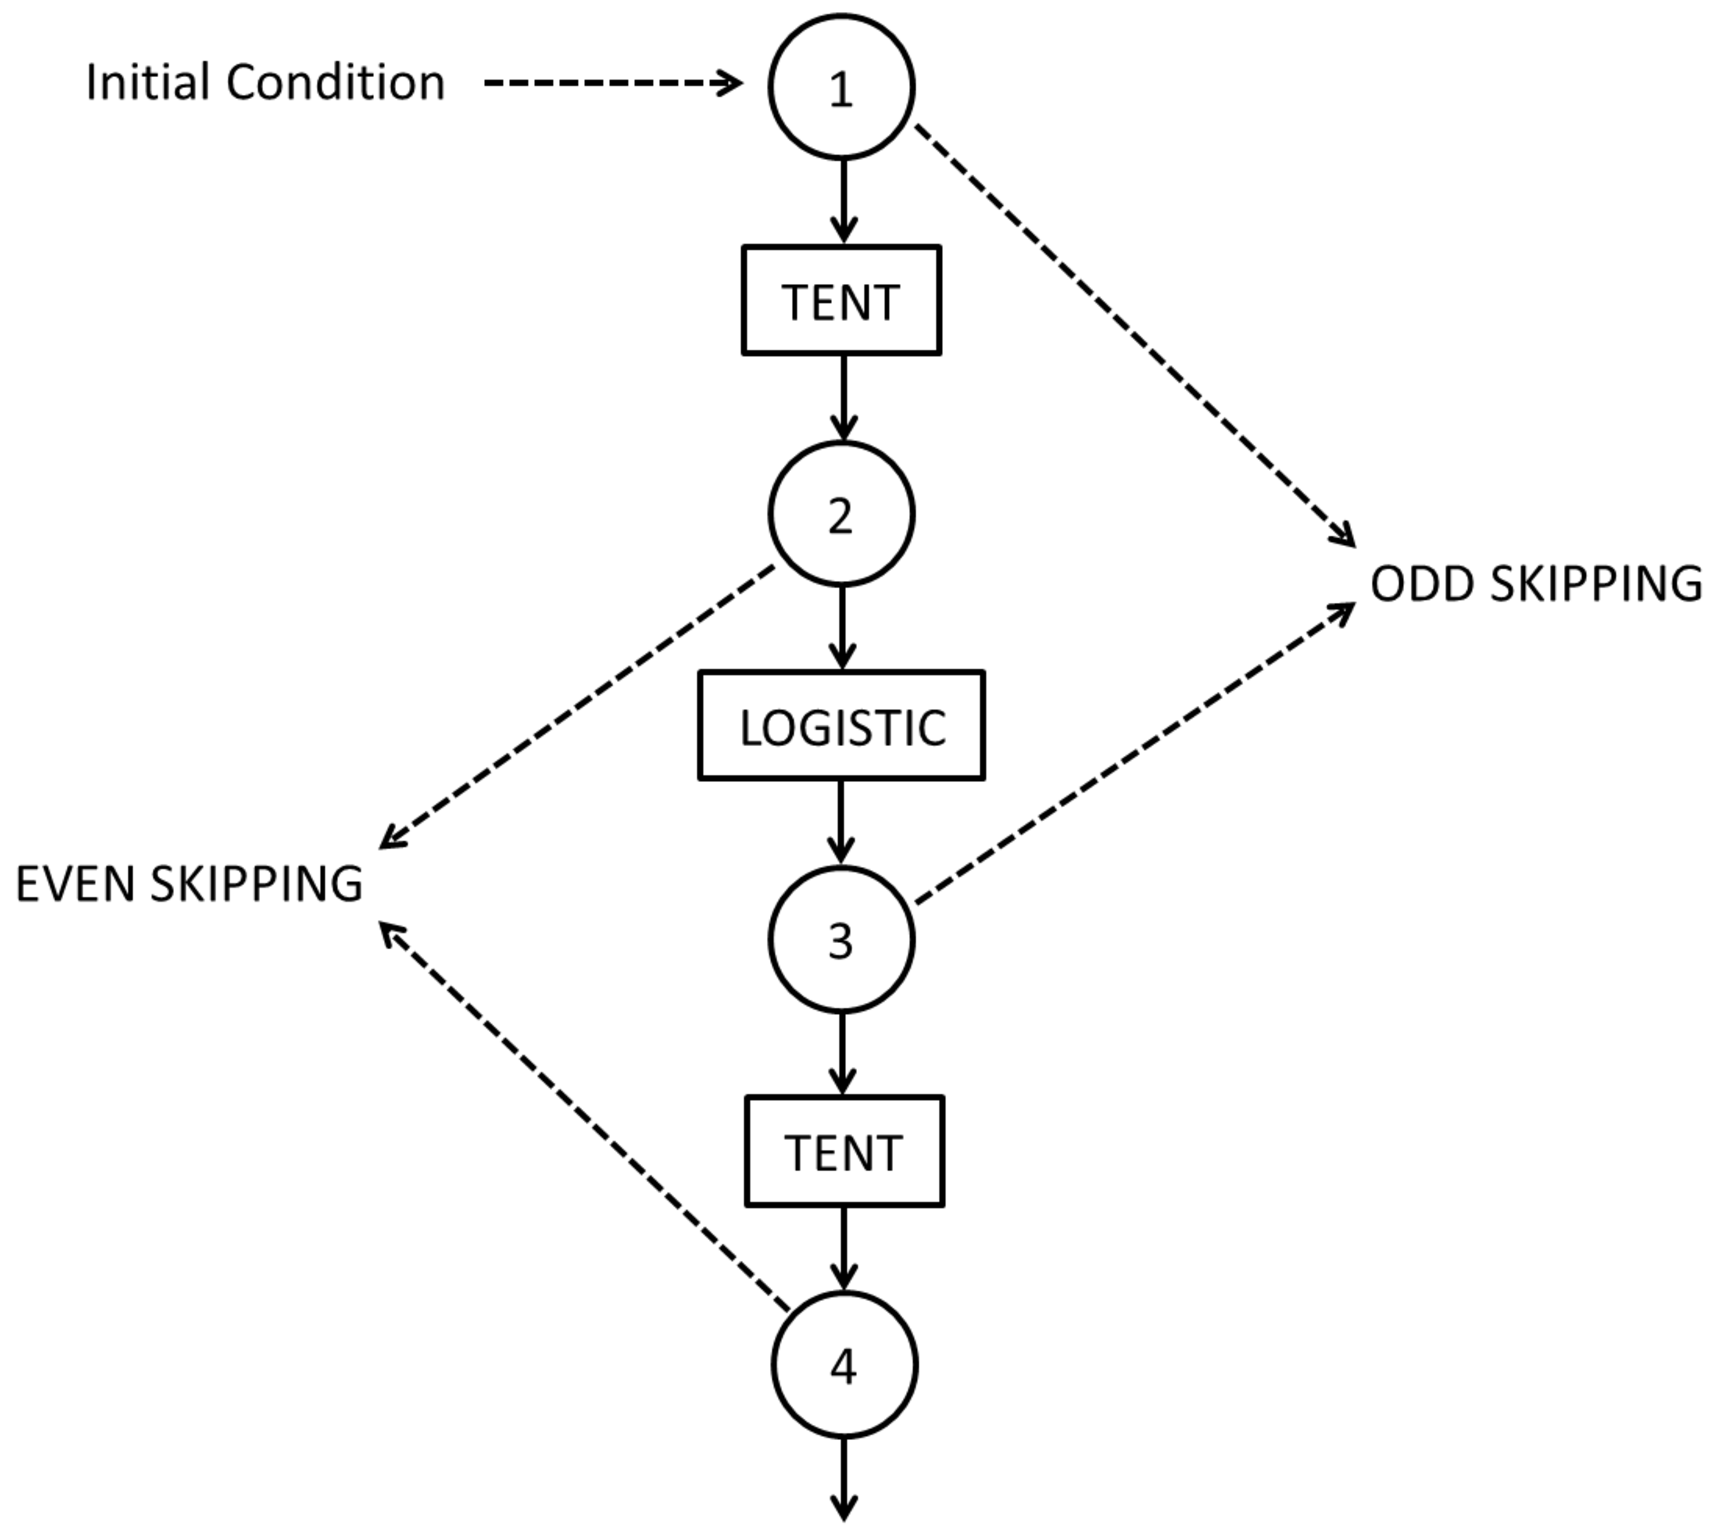
\includegraphics[height=0.4\textheight]{SwitchParImpar}
	\caption{Sequential switching between Tent and Logistic maps. In the figure are also shown even and odd skipping strategies} \label{fig:seq}
\end{figure}

The reason for studying even and odd skipping cases is the sequential switching map $M_{switch}$ is the composition of two different maps. Even skipping may be expressed as $M_{TENT}\circ M_{LOG}$ while odd skipping may be expressed as $M_{LOG}\circ M_{TENT}$.

This is very interesting to note that a great improvement is obtained using any of the skipping strategies but EVEN is slightly better than ODD.  

MP are reduced to $MP\simeq 163$ for EVEN and $MP\simeq 164$ for ODD, increasing the maximum allowed Bandt \& Pompe entropy that reaches the mean value $<H_{BP}>\simeq 0.905$ with variance $\sigma_{H_{BP}}\simeq=0.107 \times 10^{-6}$ for EVEN, and $<H_{BP}>\simeq 0.854$ with variance $\sigma_{H_{BP}}\simeq=0.285 \times 10^{-6}$ for a decimal representation with  $9\leq P\leq27$. The complexity is reduced to $<C_{BP}>\simeq 0.224$ with $\sigma_{C_{BP}}\simeq=0.166 \times 10^{-6}$ for EVEN and  $<C_{BP}>\simeq 0.282$ with $\sigma_{C_{BP}}\simeq=0.281 \times 10^{-6}$ for ODD.

Quantifiers related to the normalized histogram slightly degrades with the skipping procedure. For example $H_{hist}$ reduces from $0.866$ without skipping to $0.813$ for any EVEN or ODD. 

Results in binary numbers are similar to those obtained for the equivalent number of figures in decimal numbers. For example the minimum in MP is reached for $B=27$, and this number of bits is almost equivalent to $P=9$. 

In Figs. \ref{fig:seqpardec} and Figs. \ref{fig:seqparbin} are shown the results for EVEN. We do not give the Figs. for ODD because they are very similar, as pointed above.

\begin{figure}
	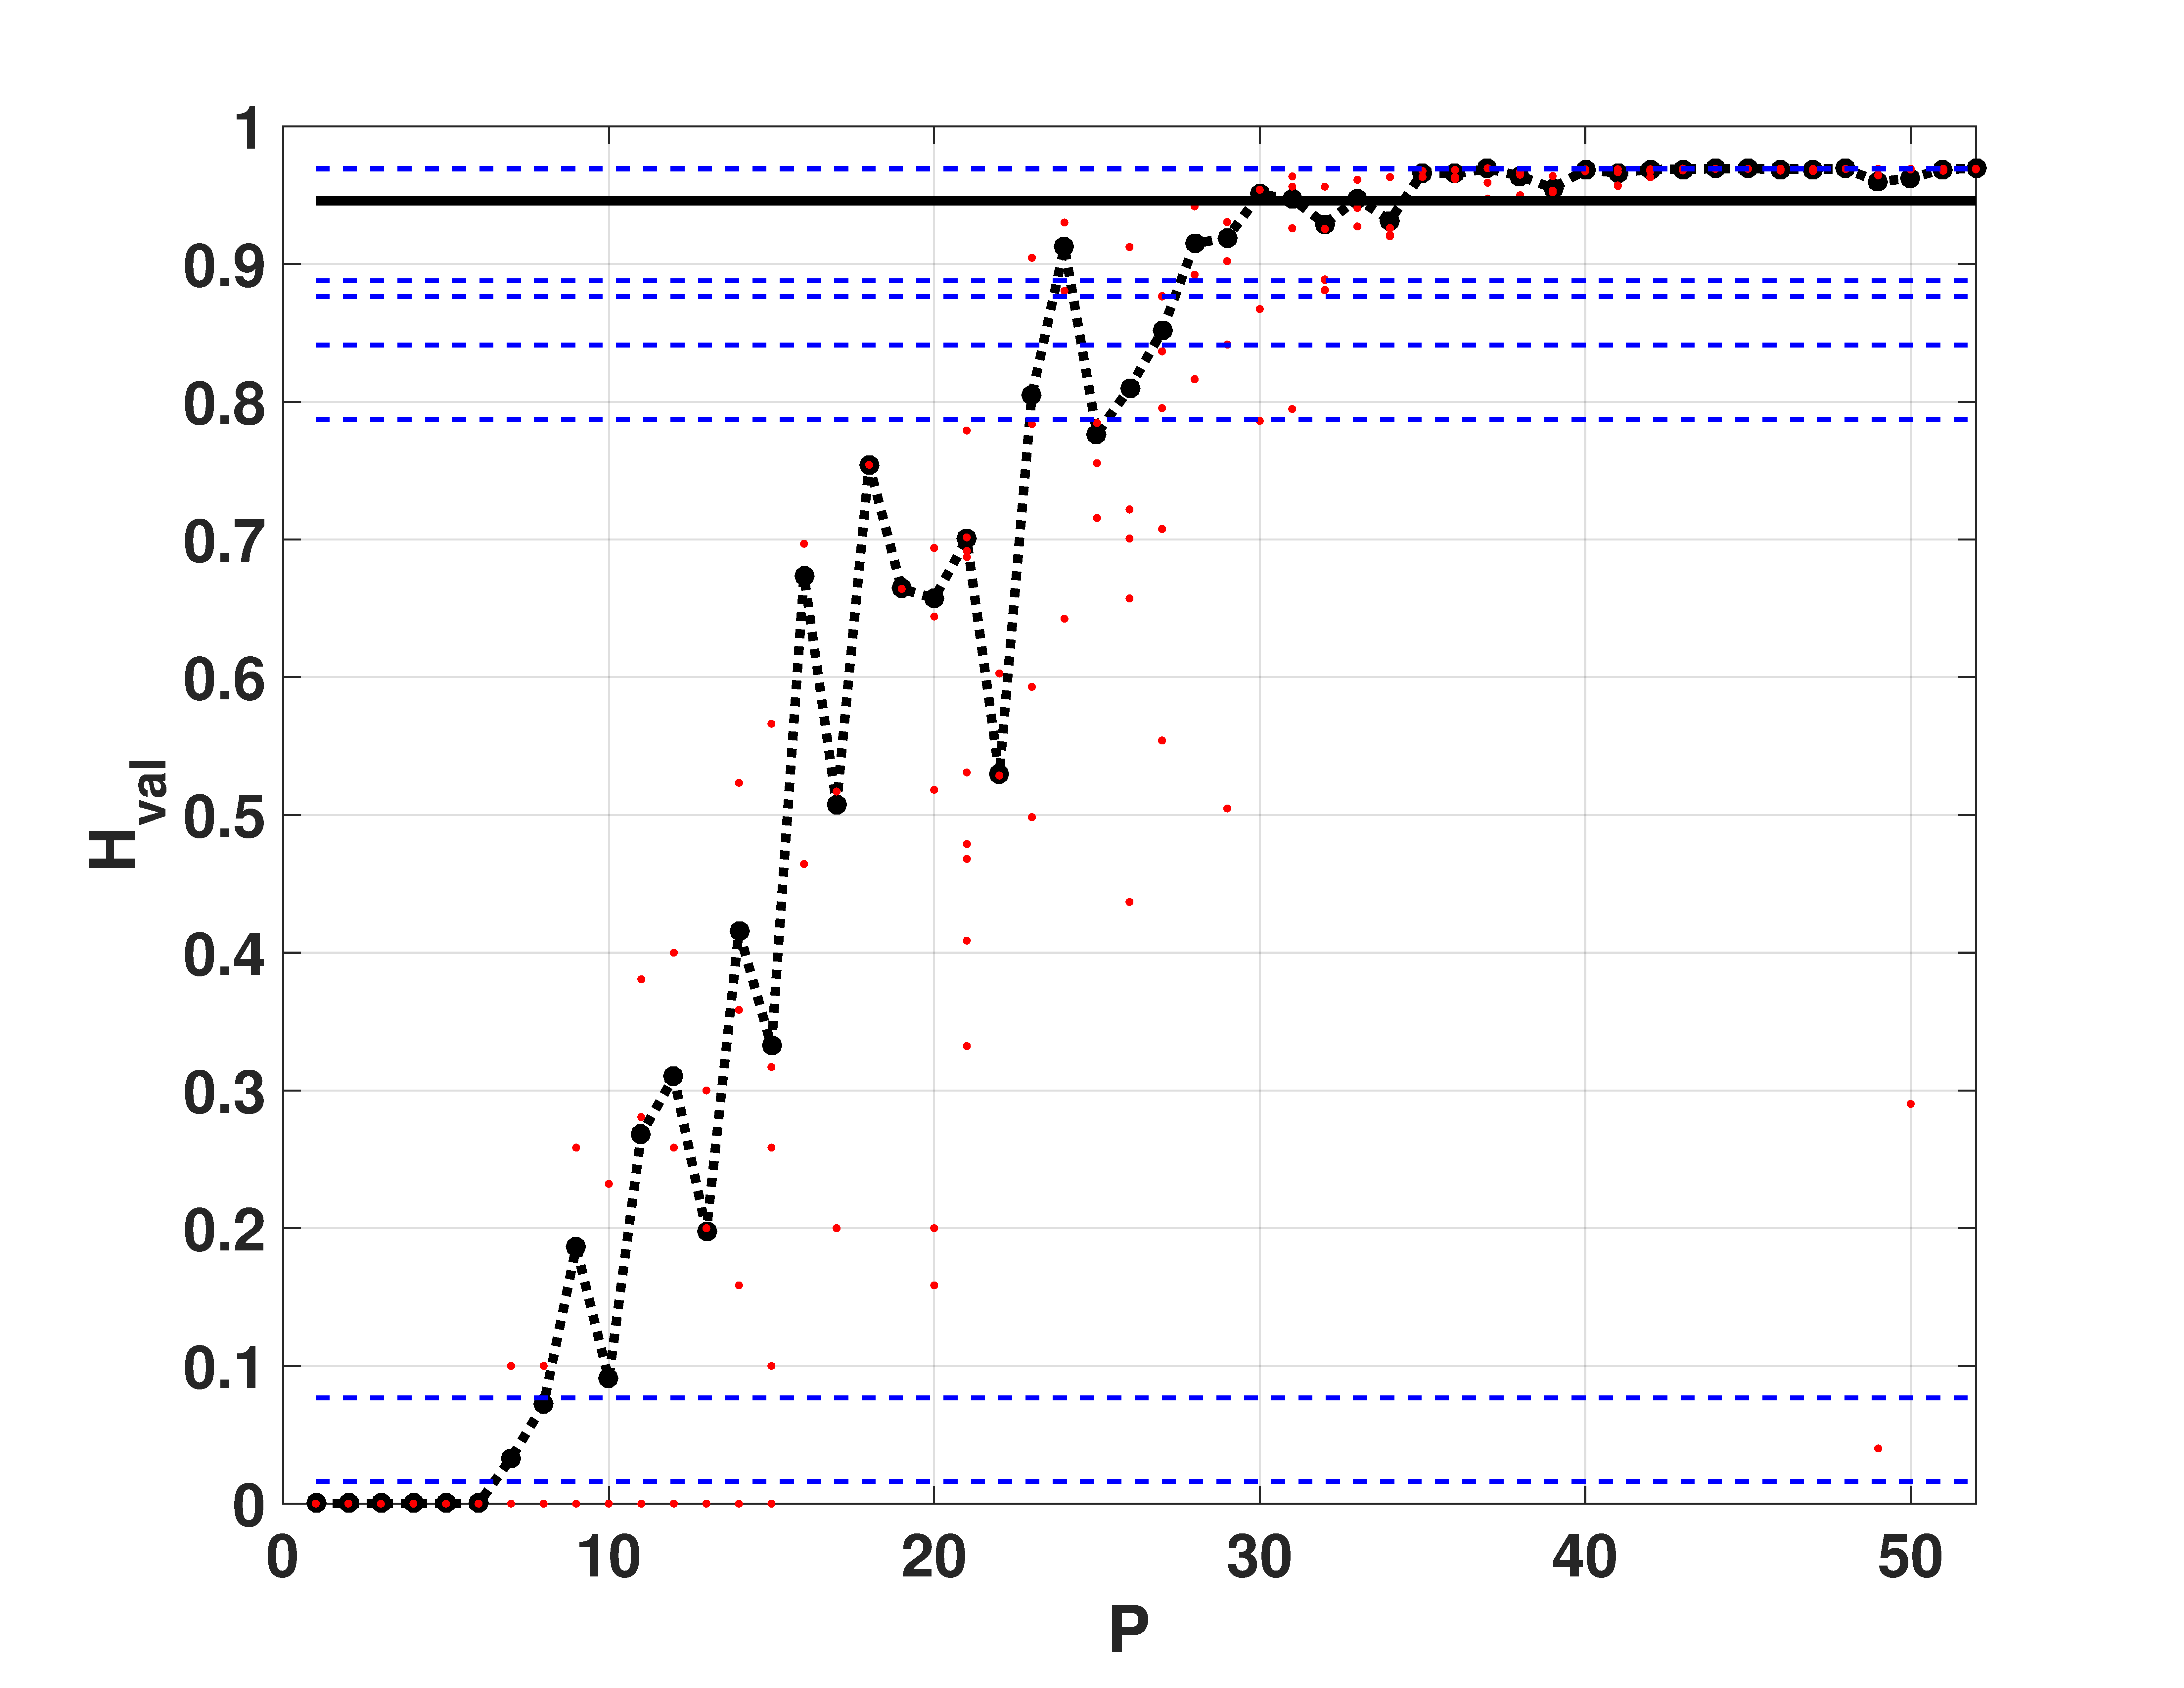
\includegraphics[width=.32\textwidth]{Hval_SwitchEven}
	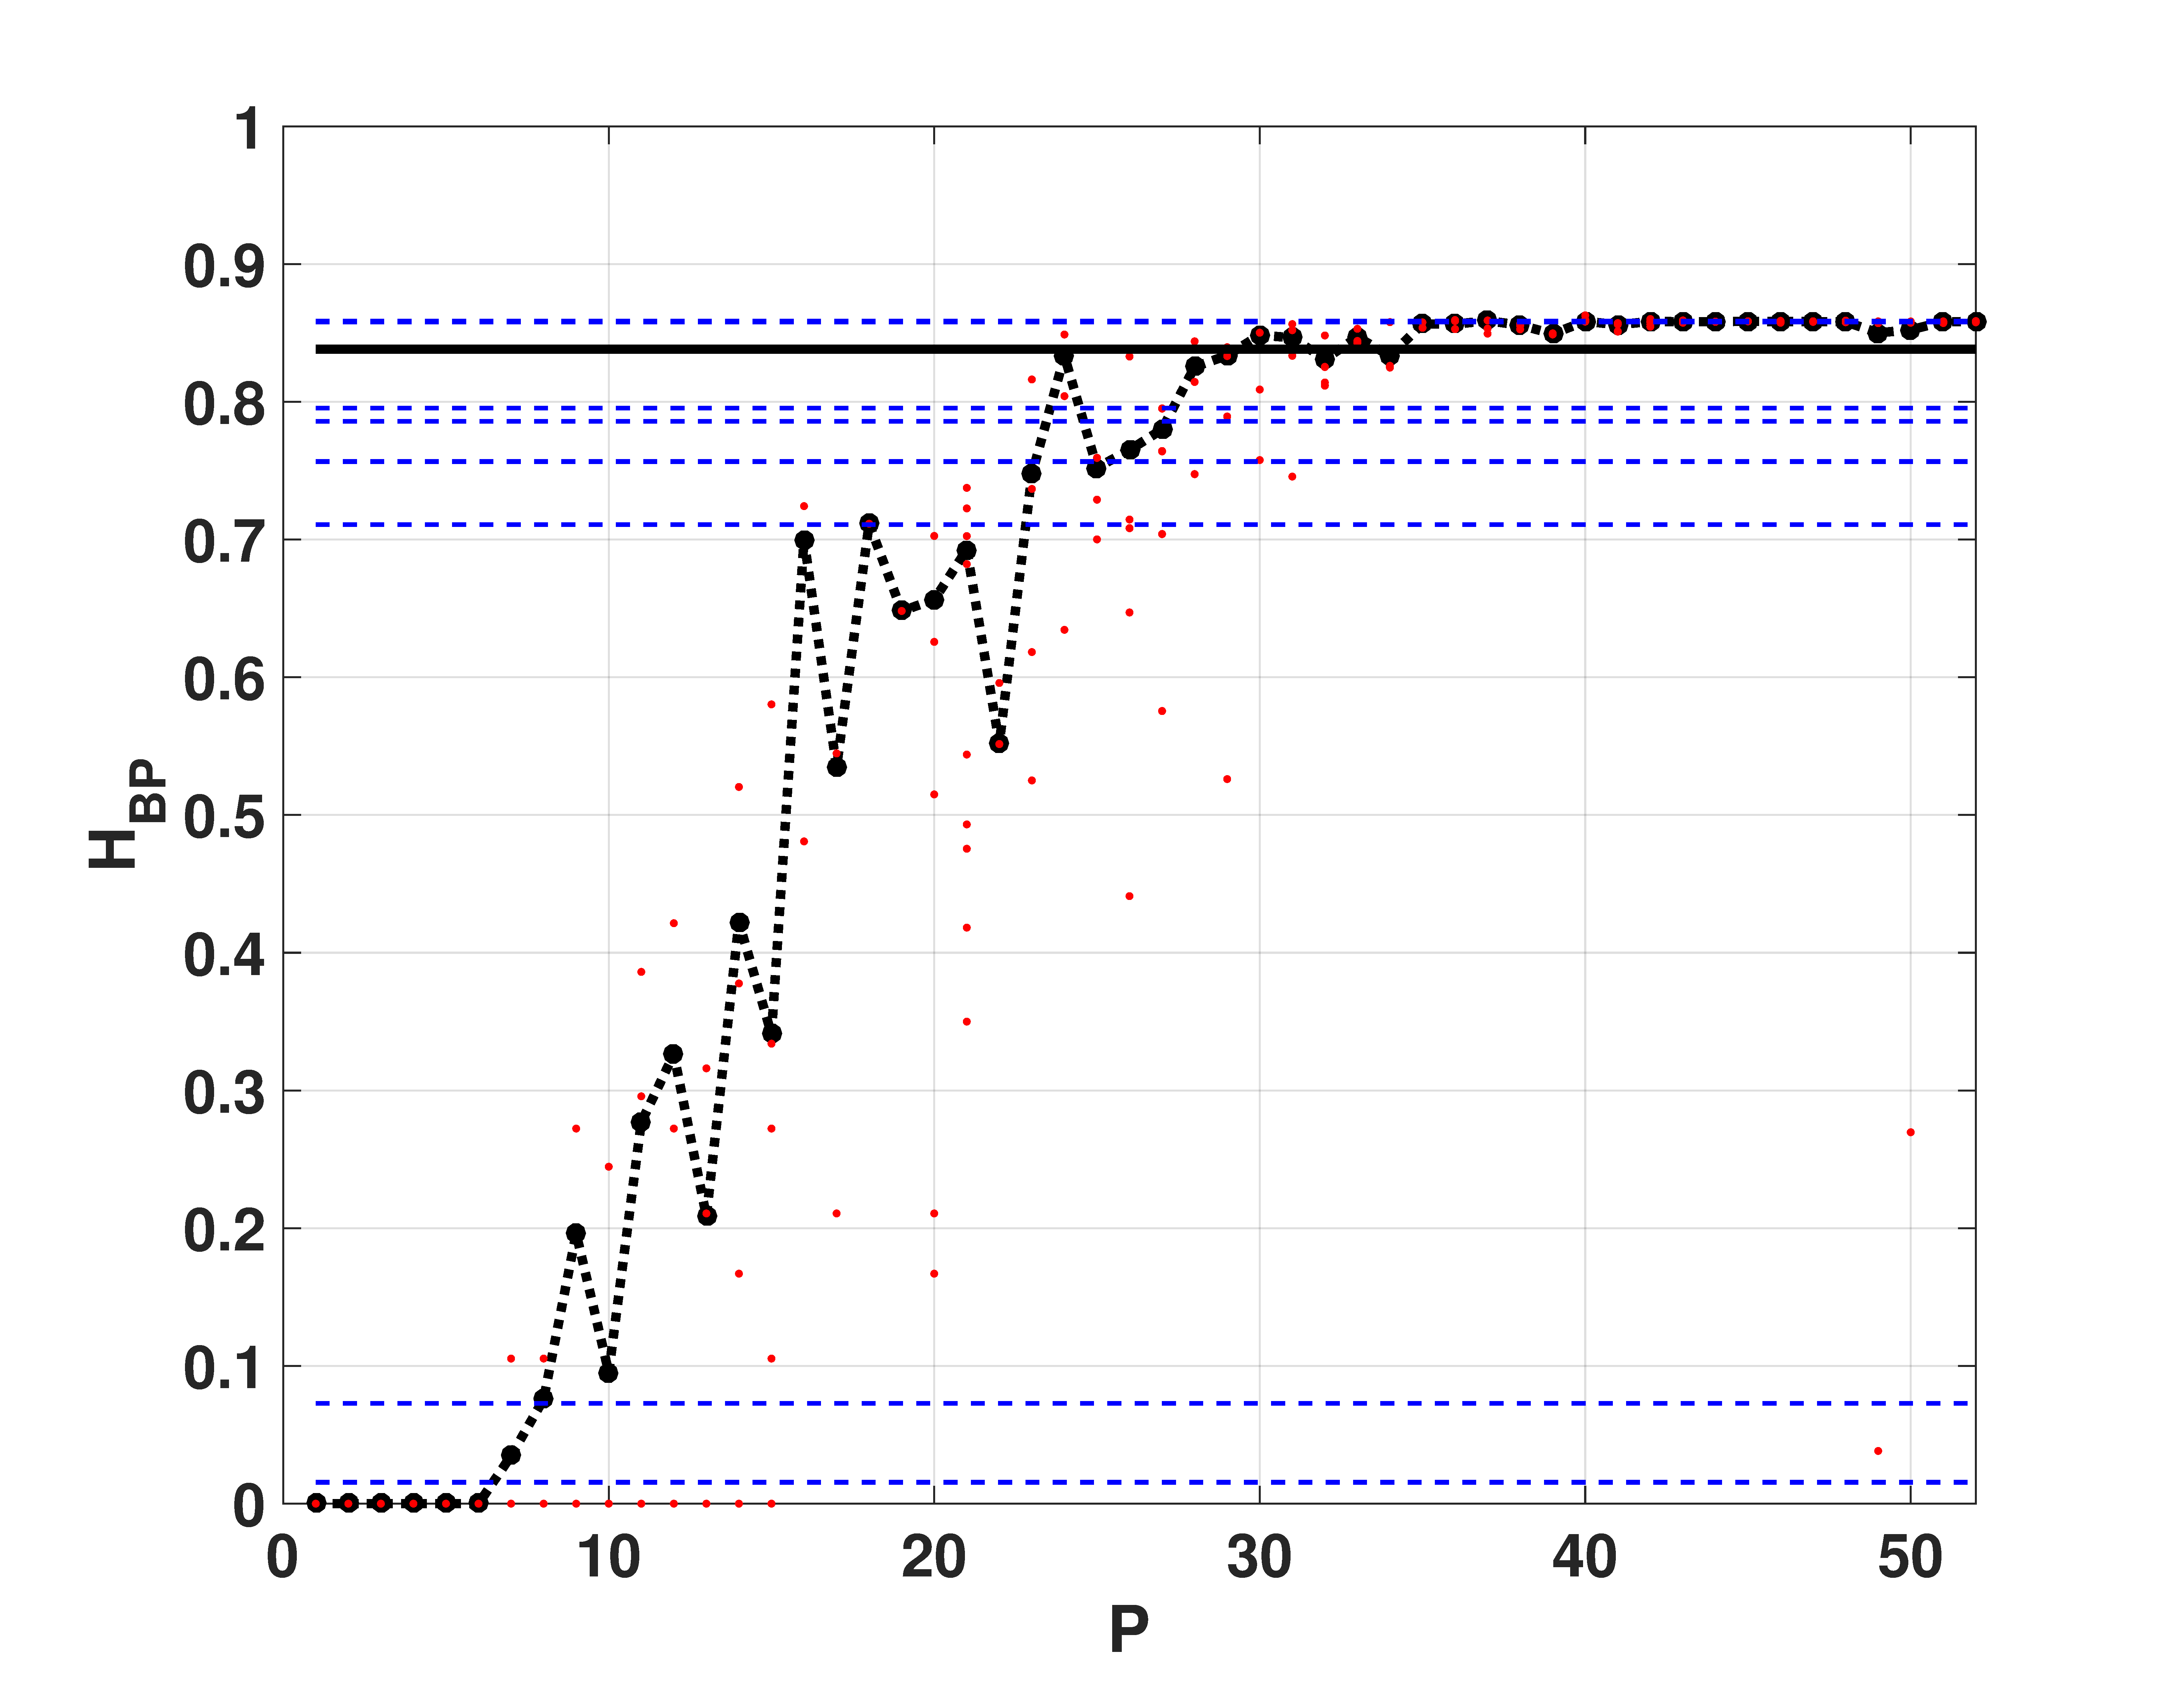
\includegraphics[width=.32\textwidth]{Hbp_SwitchEven}
	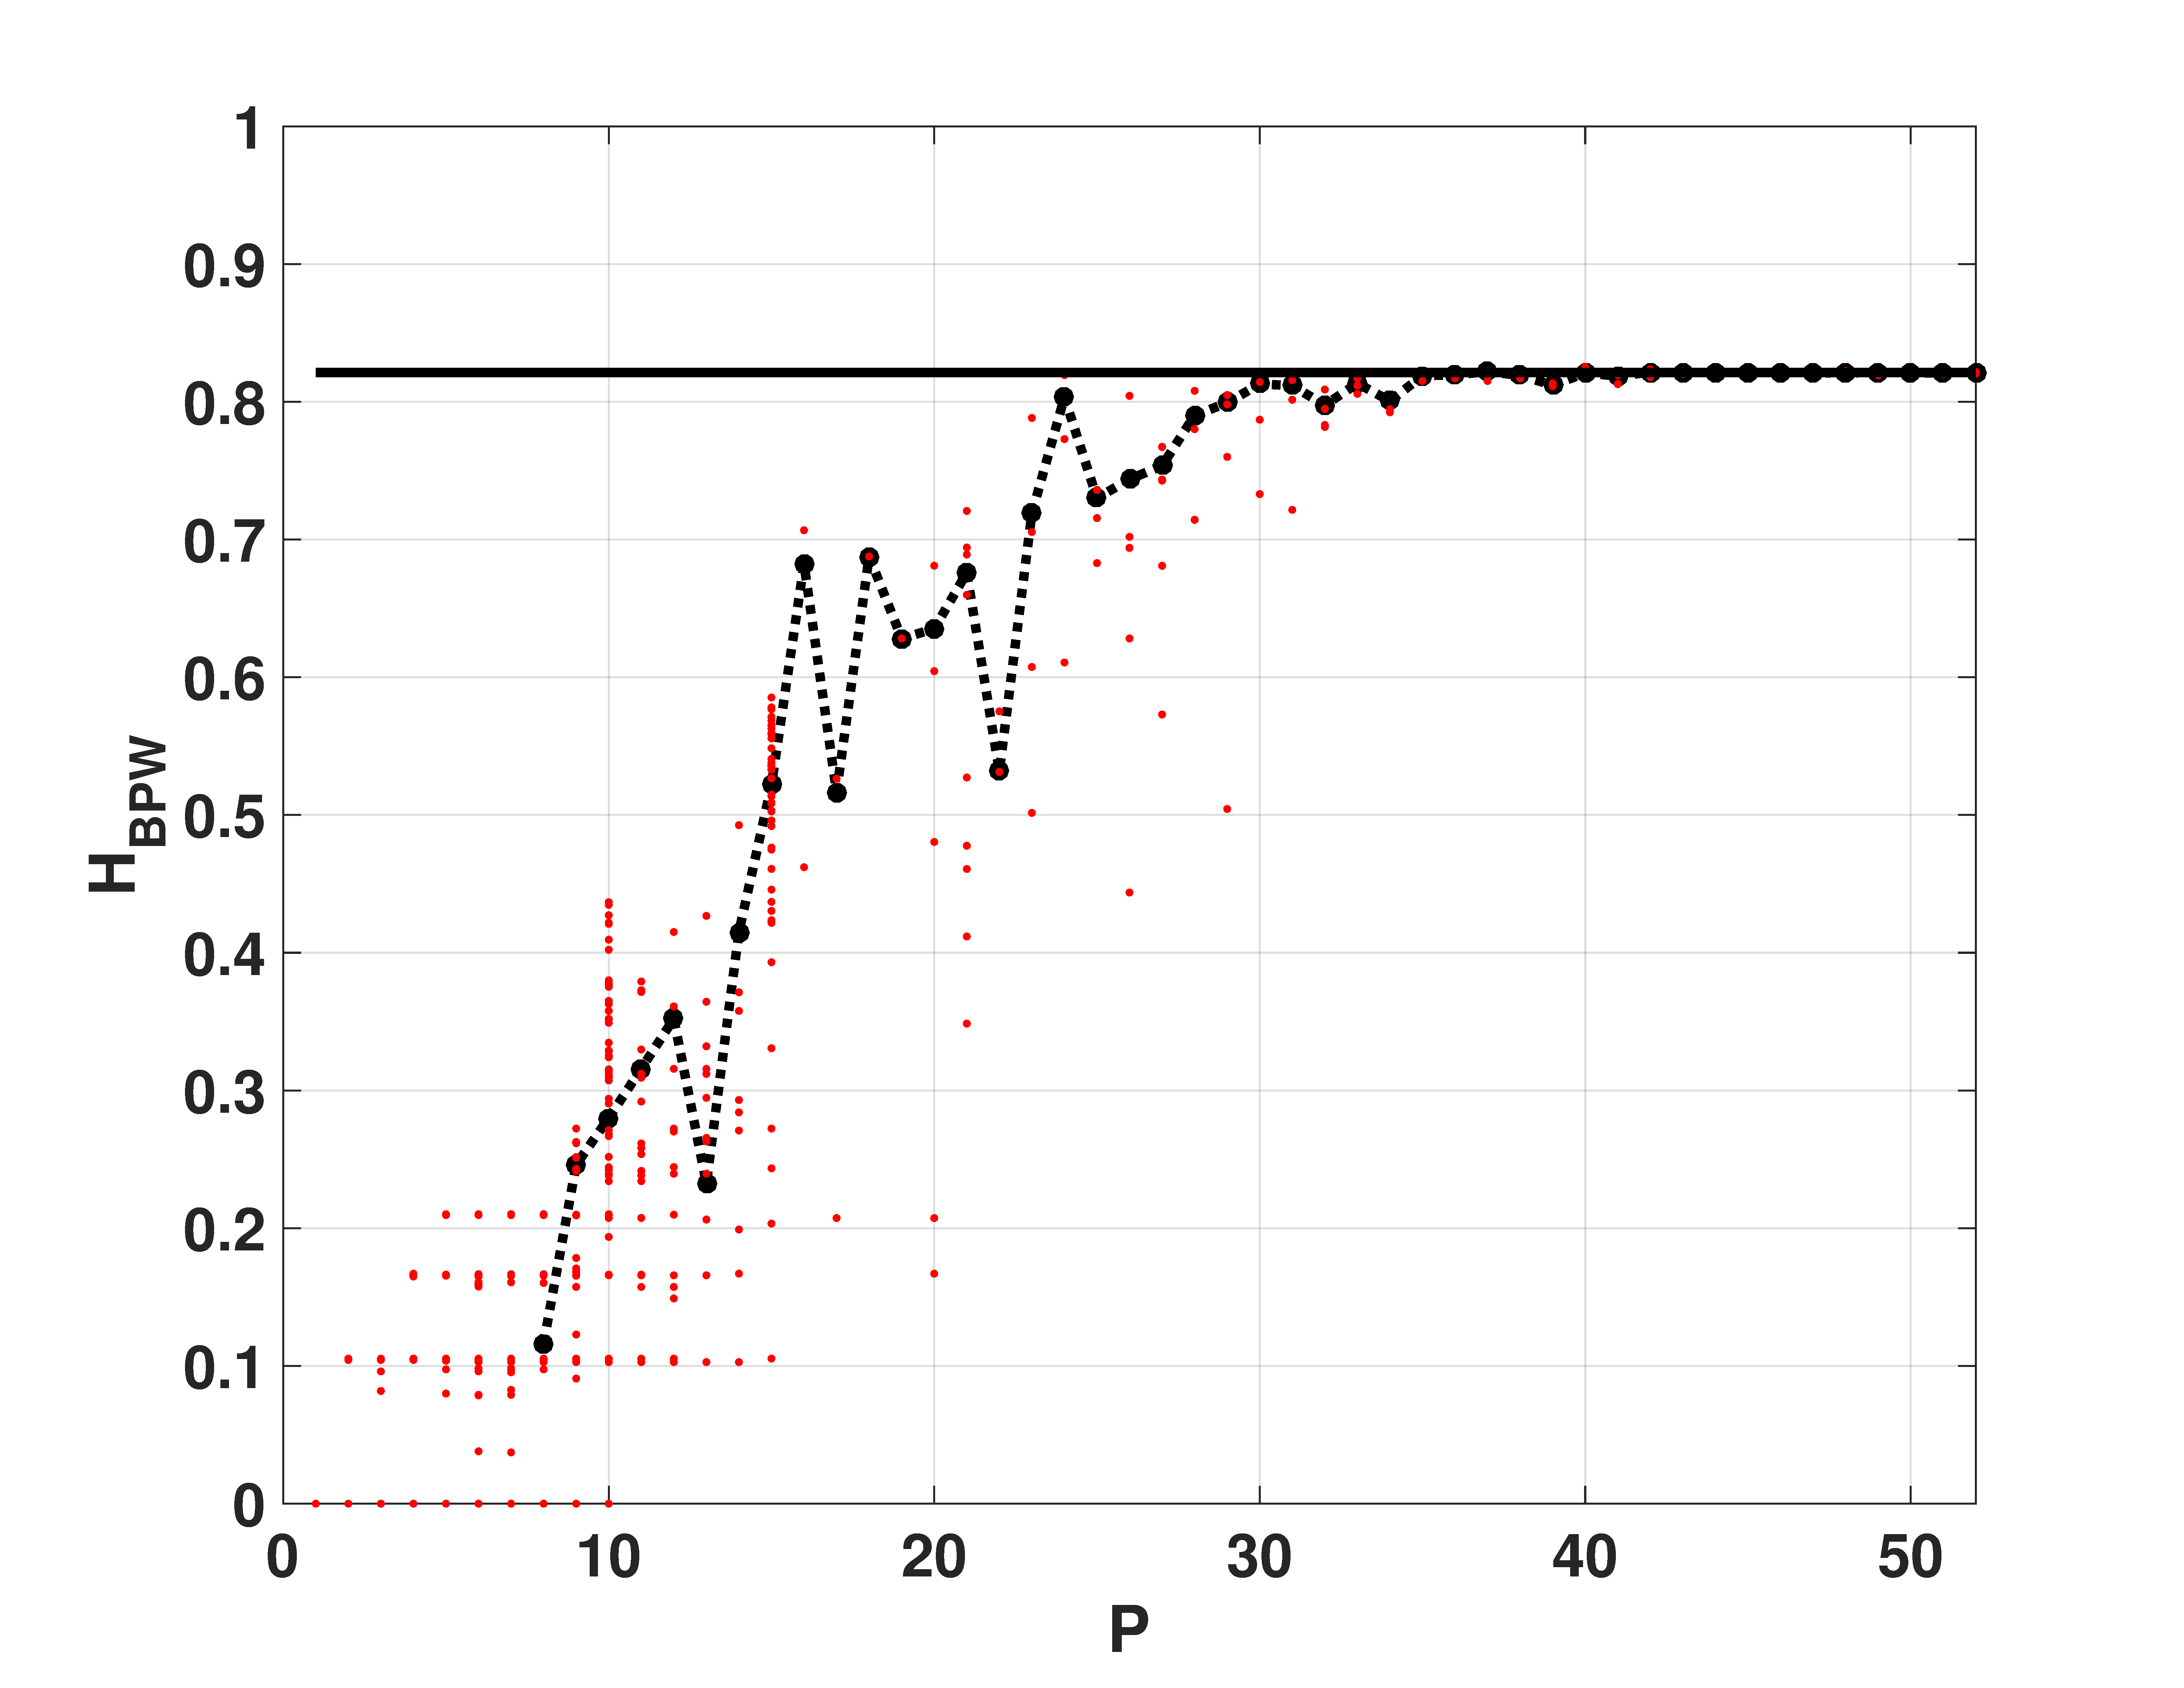
\includegraphics[width=.32\textwidth]{Hbpw_SwitchEven}
	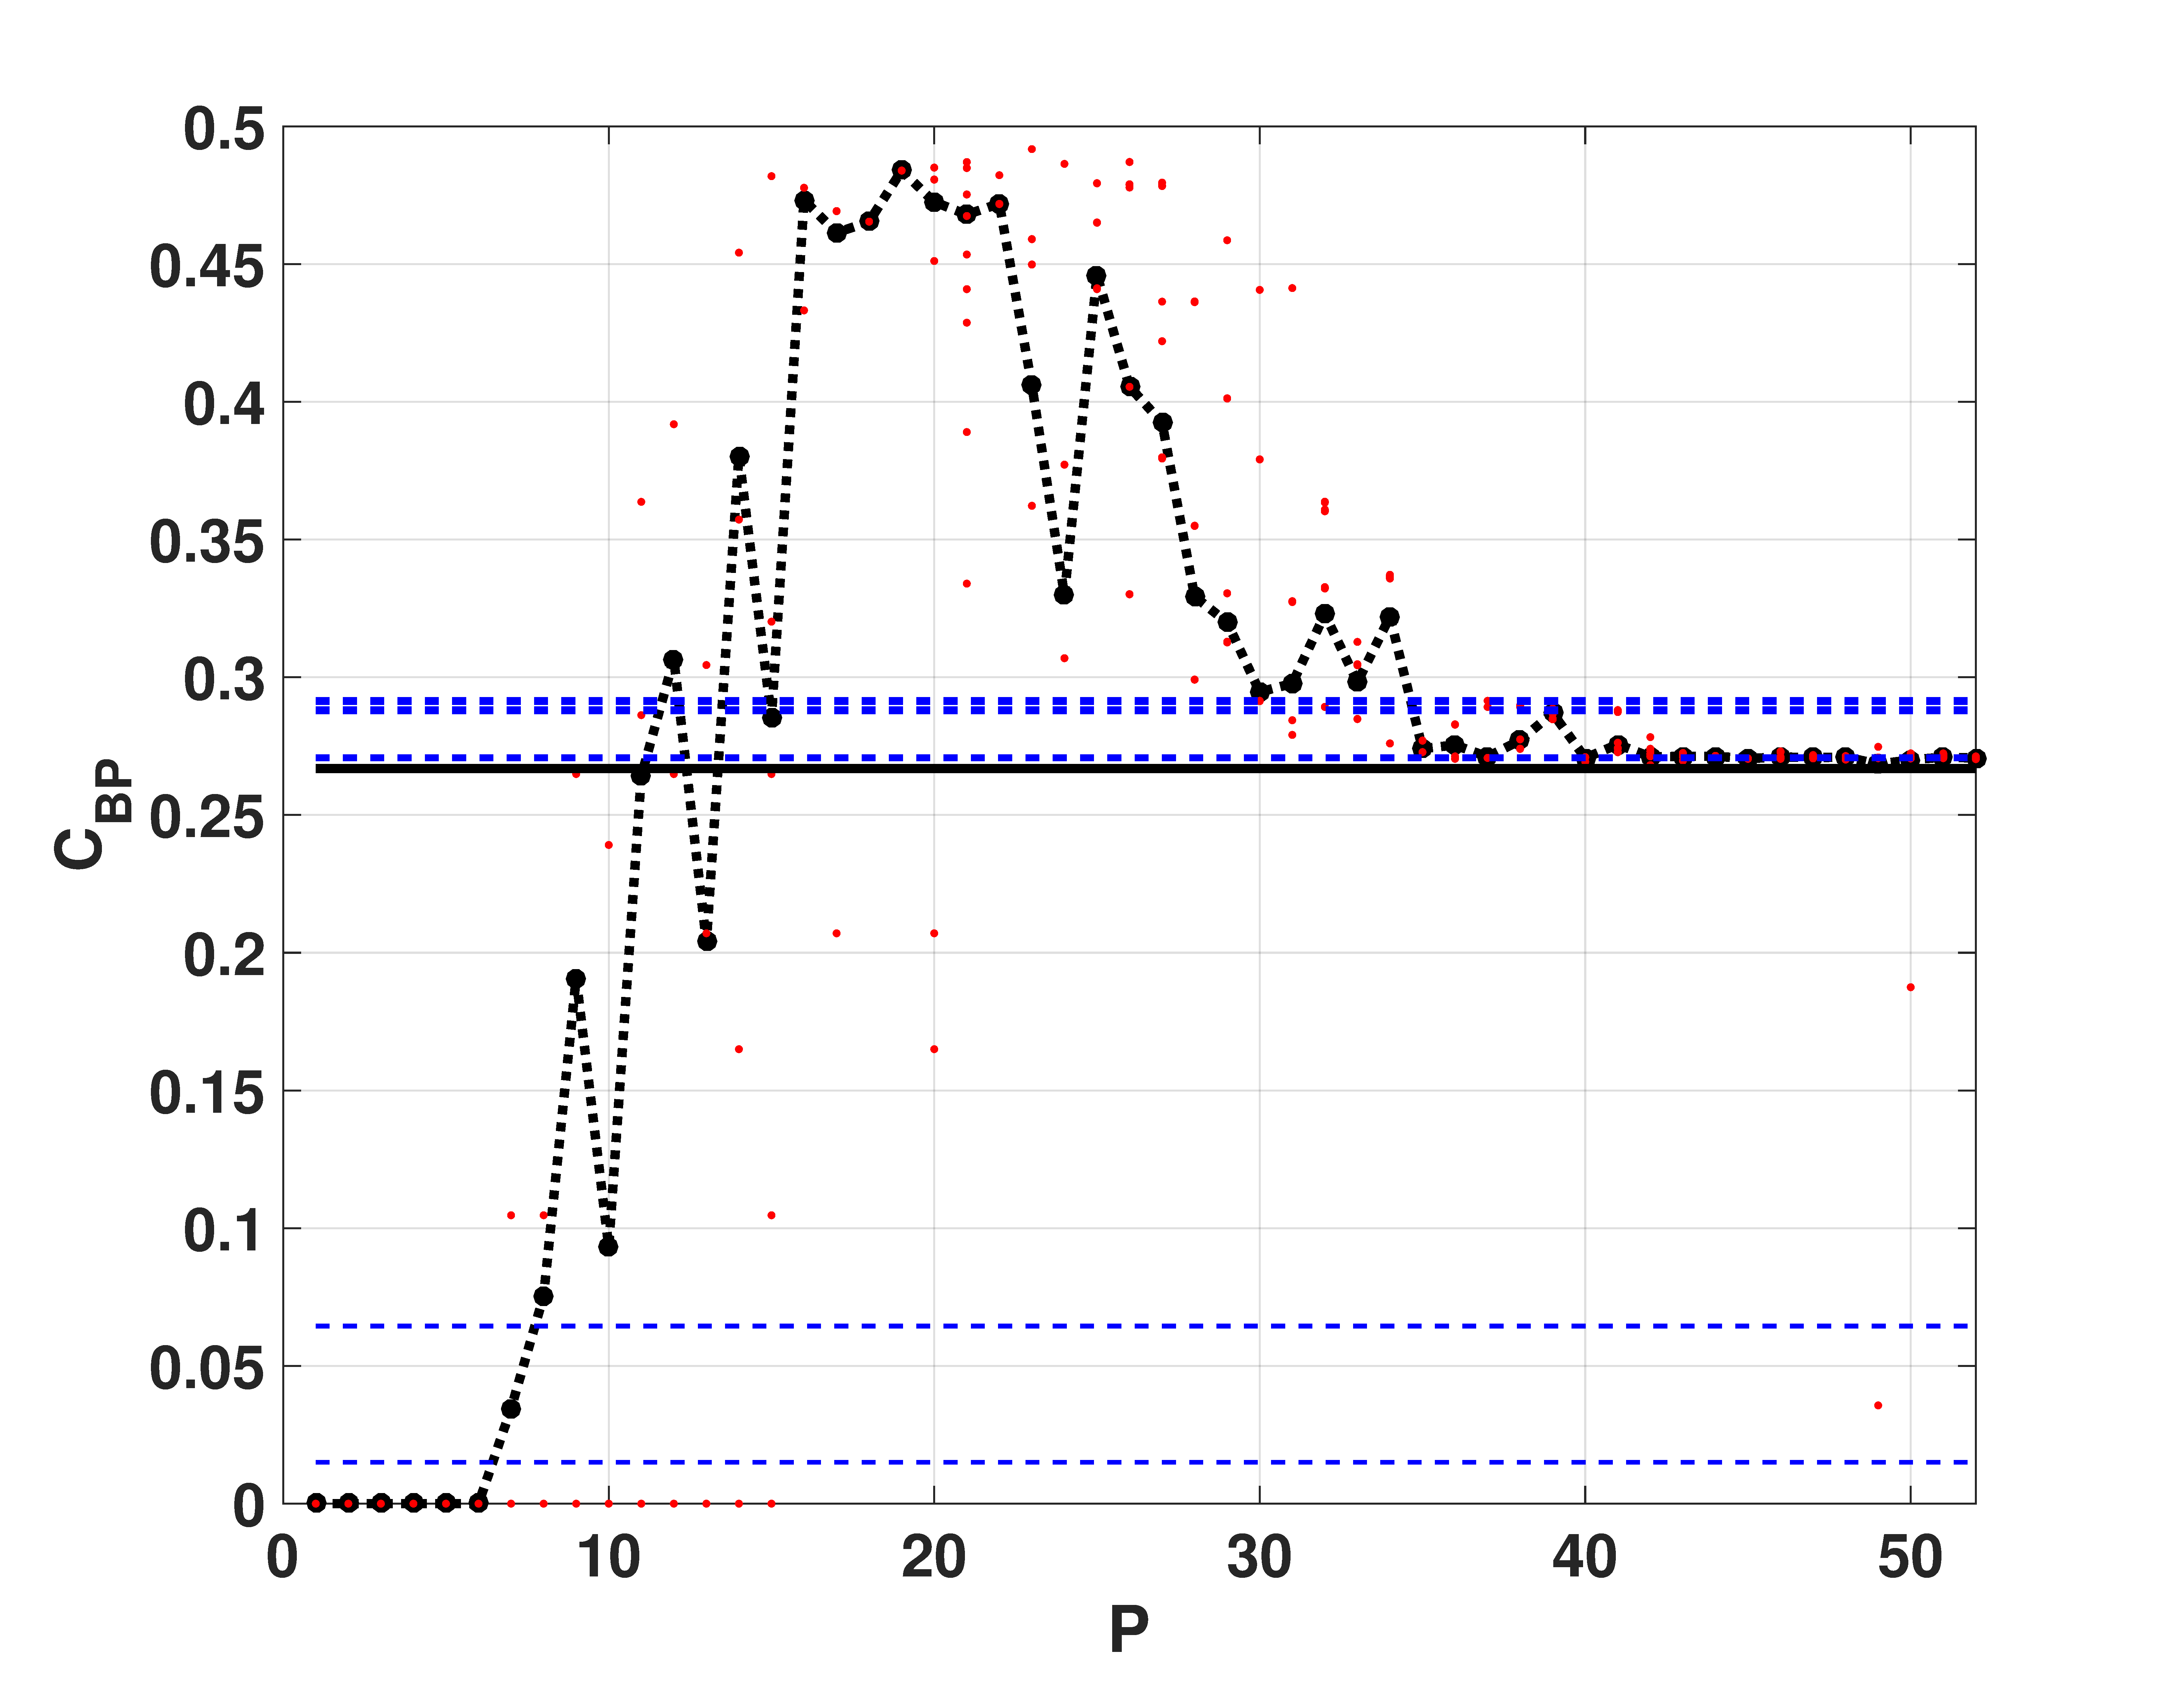
\includegraphics[width=.32\textwidth]{Cbp_SwitchEven}
	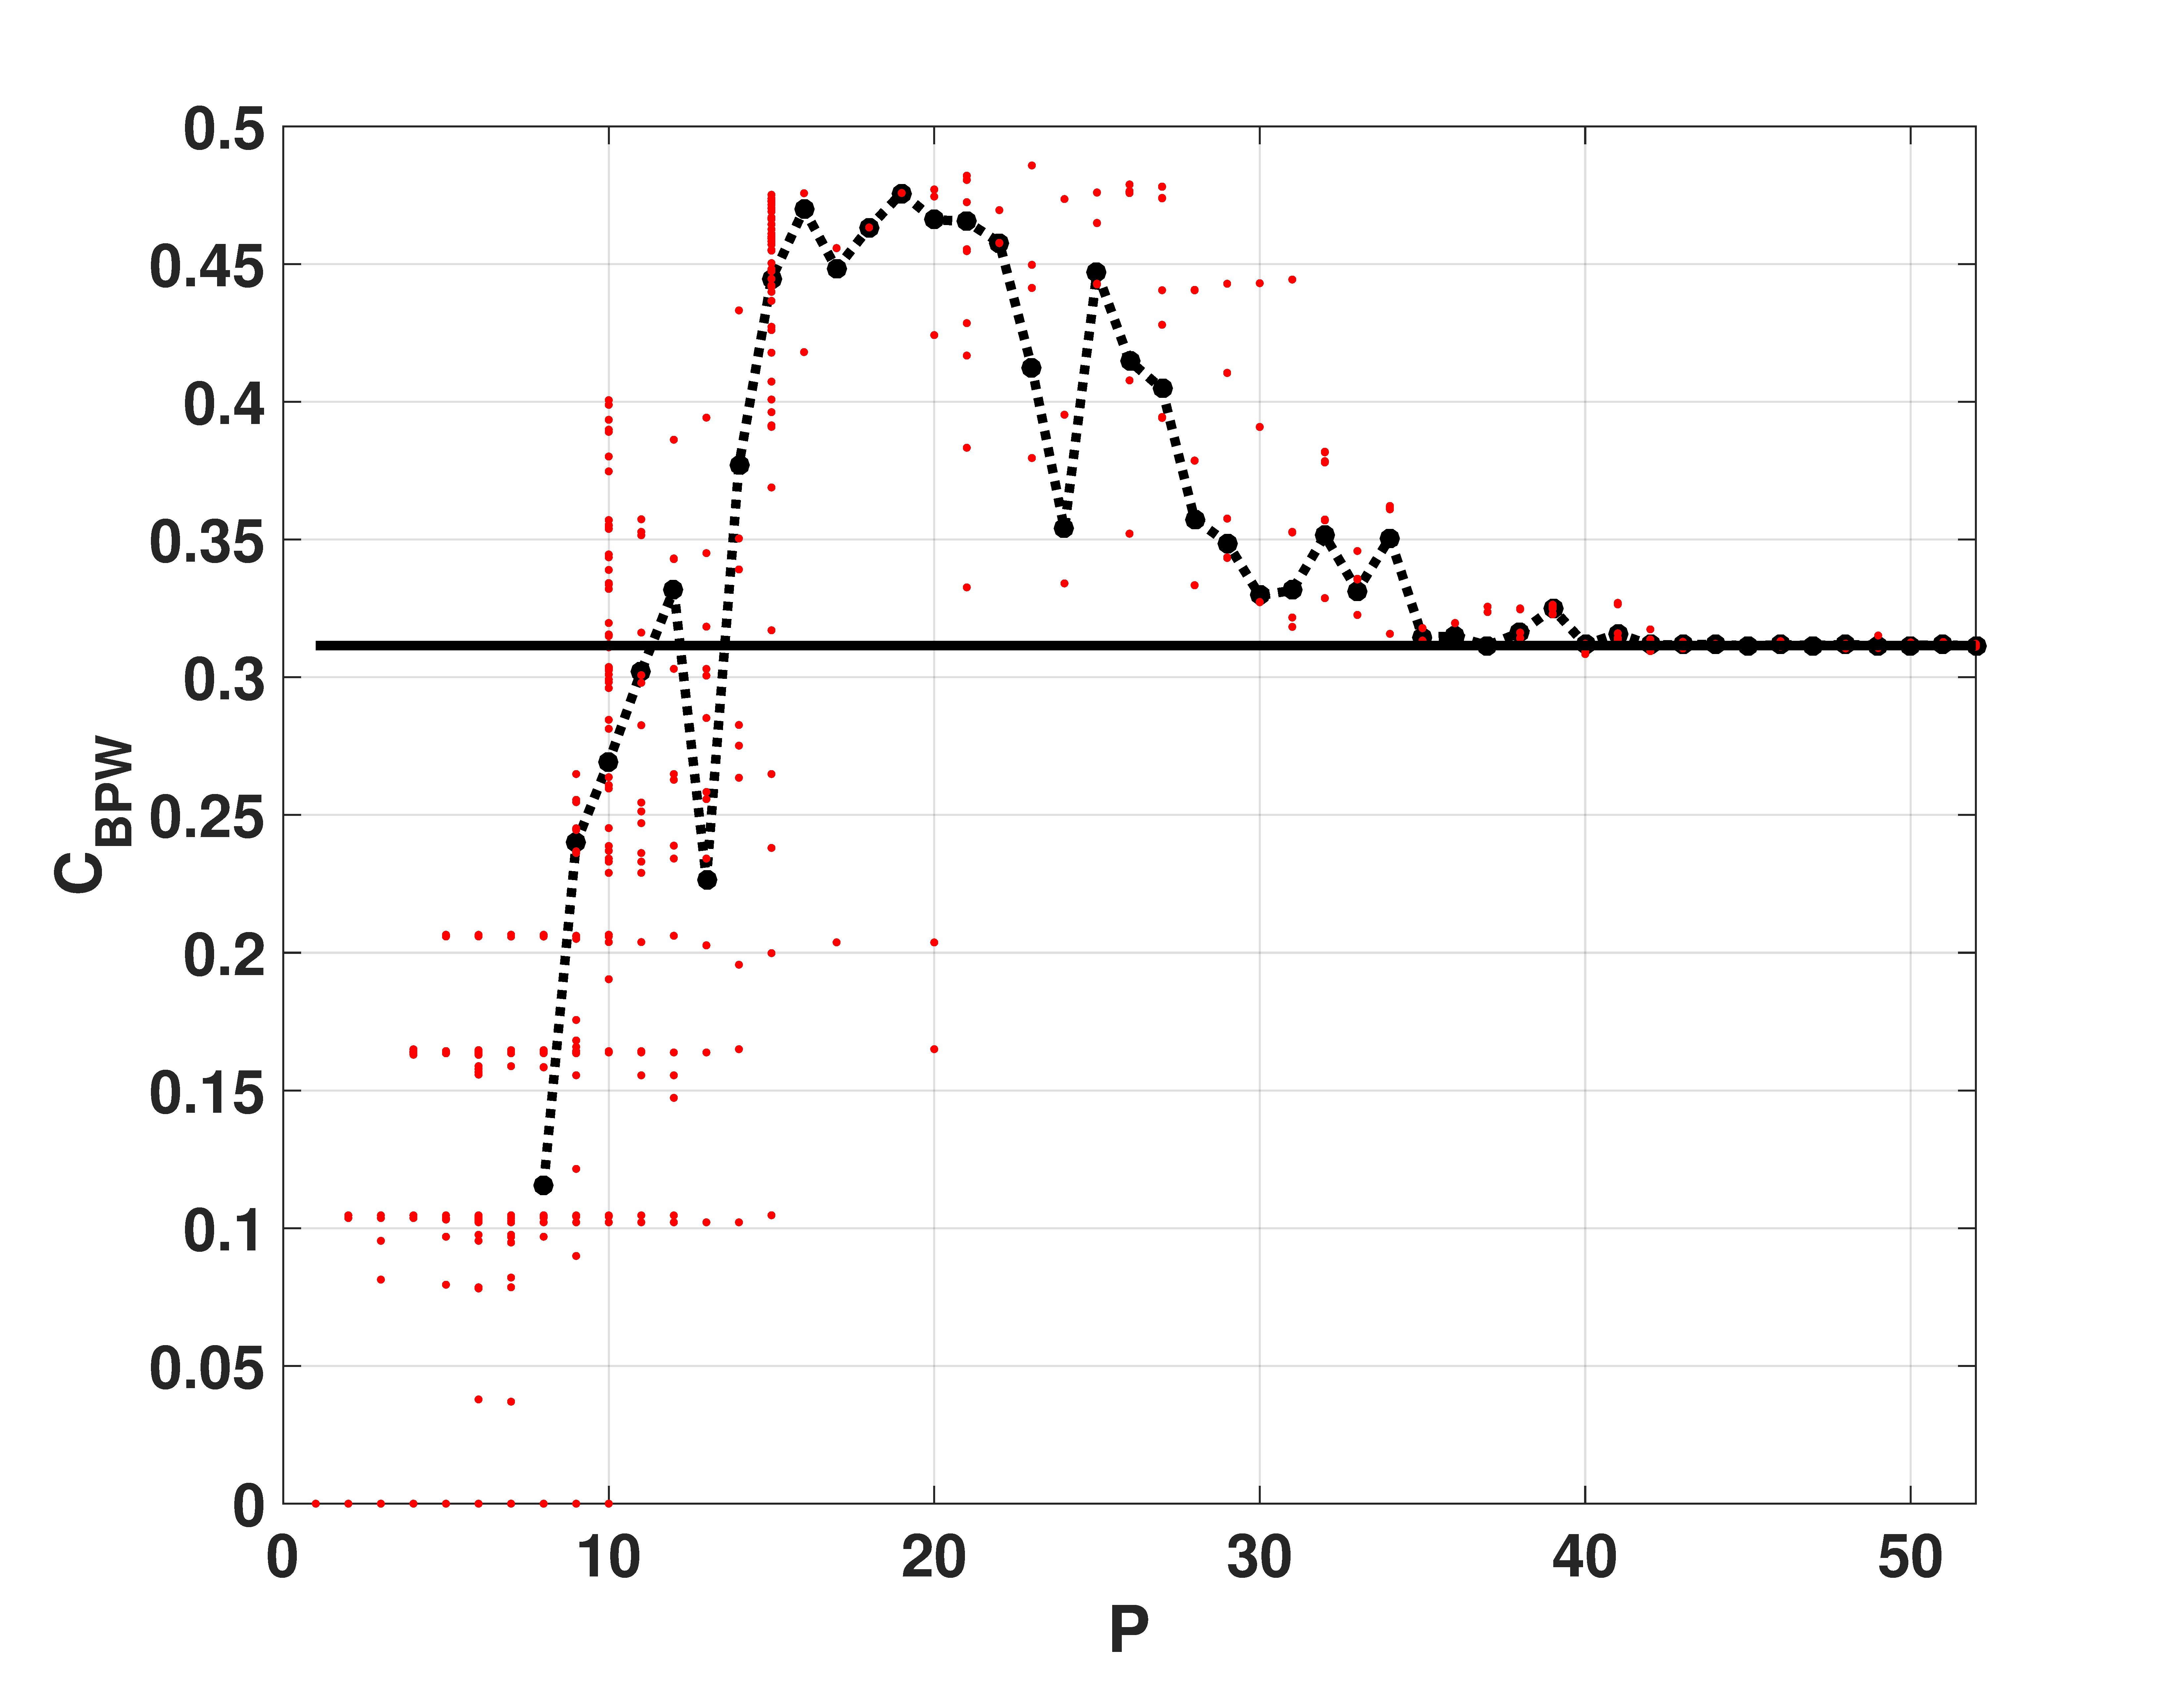
\includegraphics[width=.32\textwidth]{Cbpw_SwitchEven}
	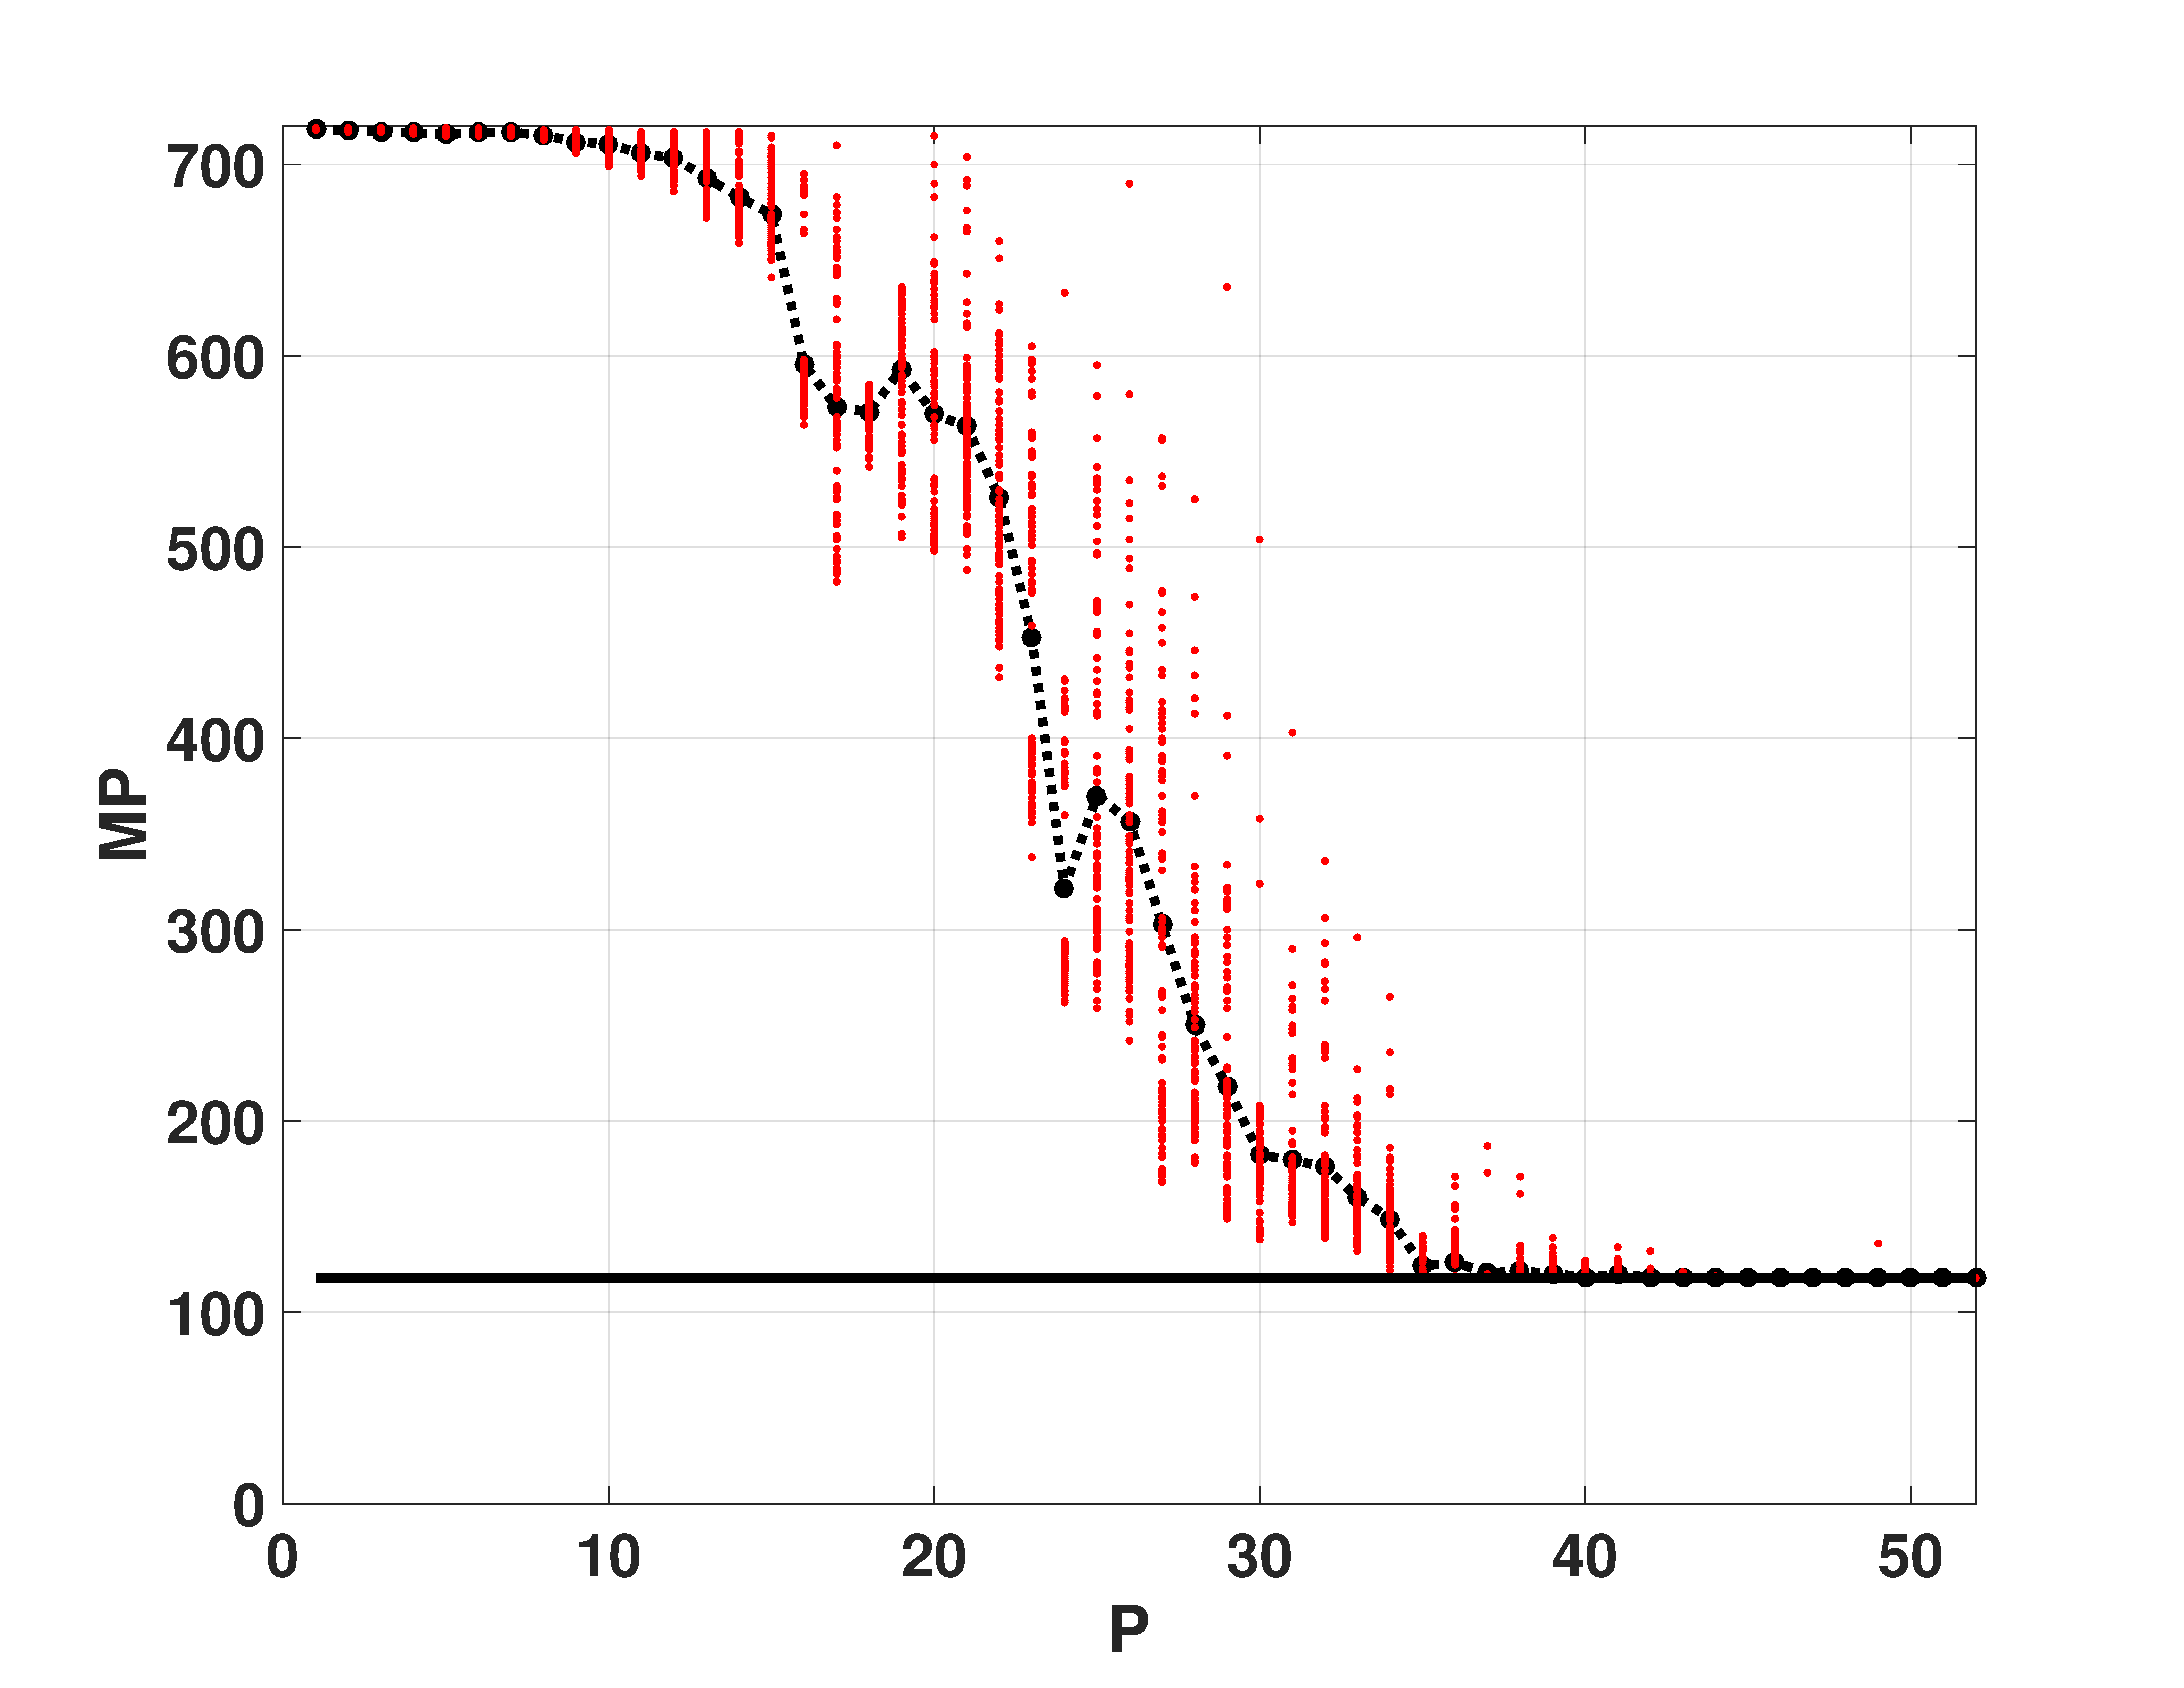
\includegraphics[width=.32\textwidth]{MP_SwitchEven}
	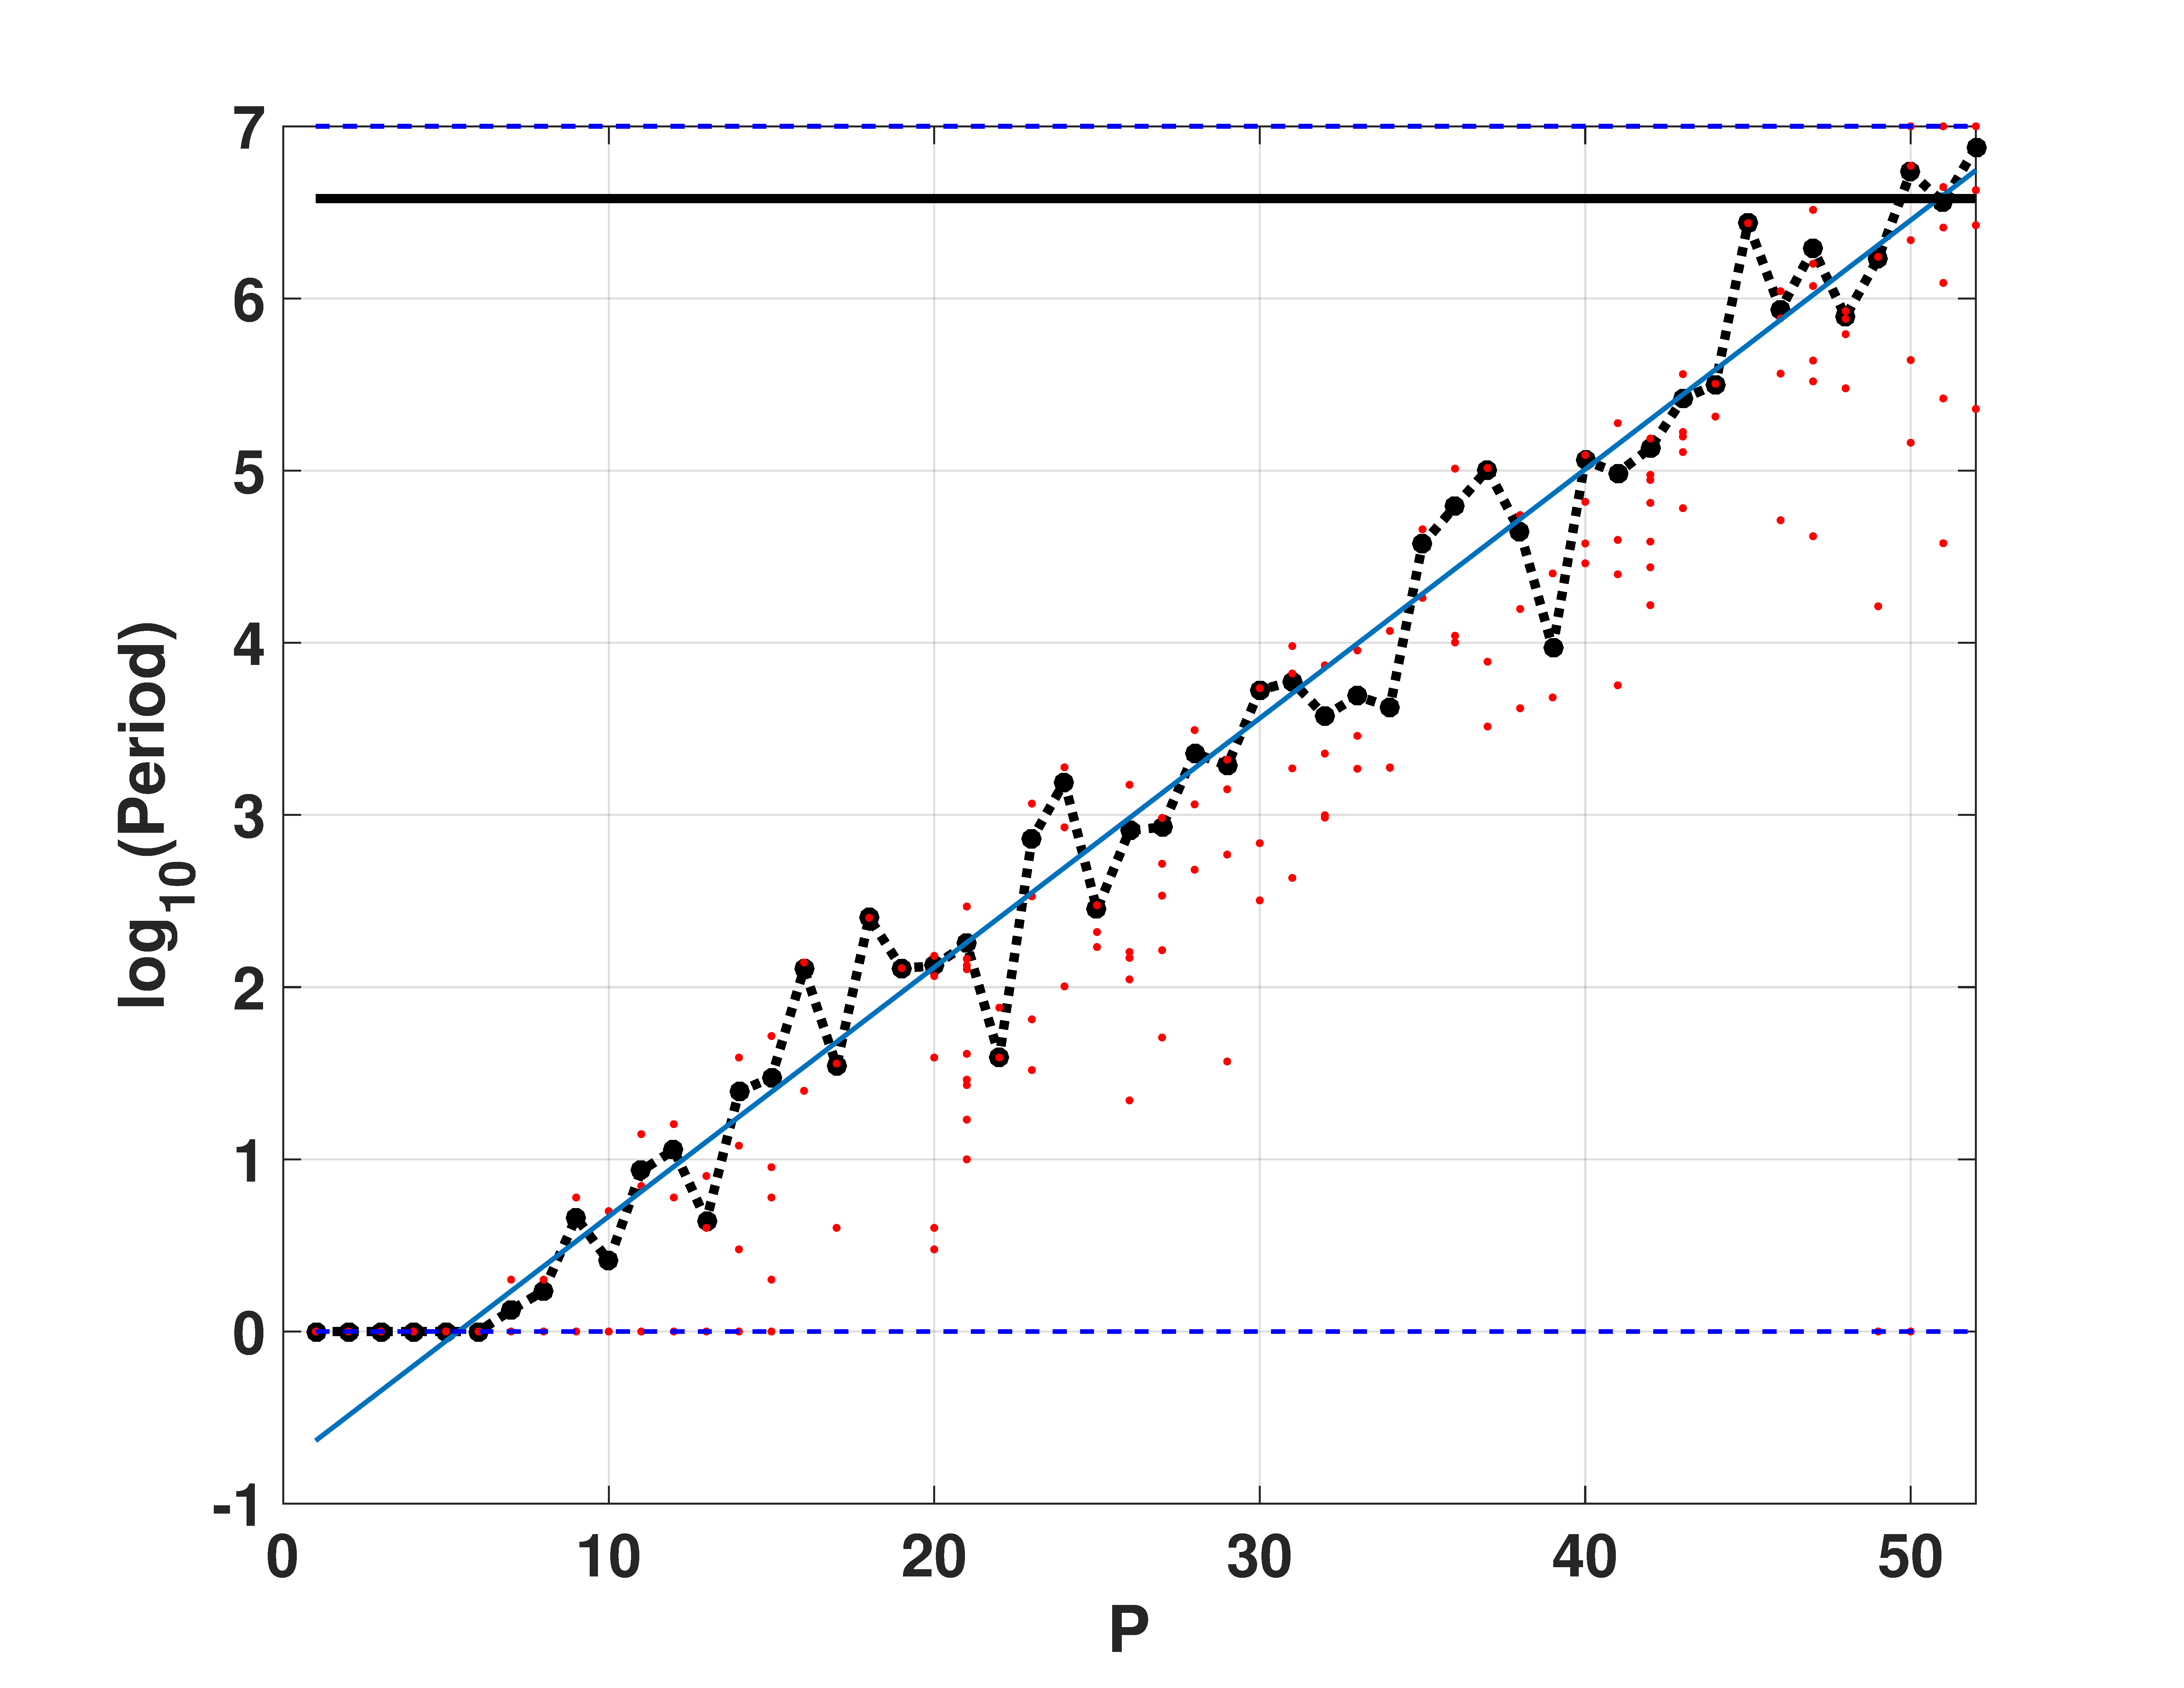
\includegraphics[width=.32\textwidth]{Period_SwitchEven}
	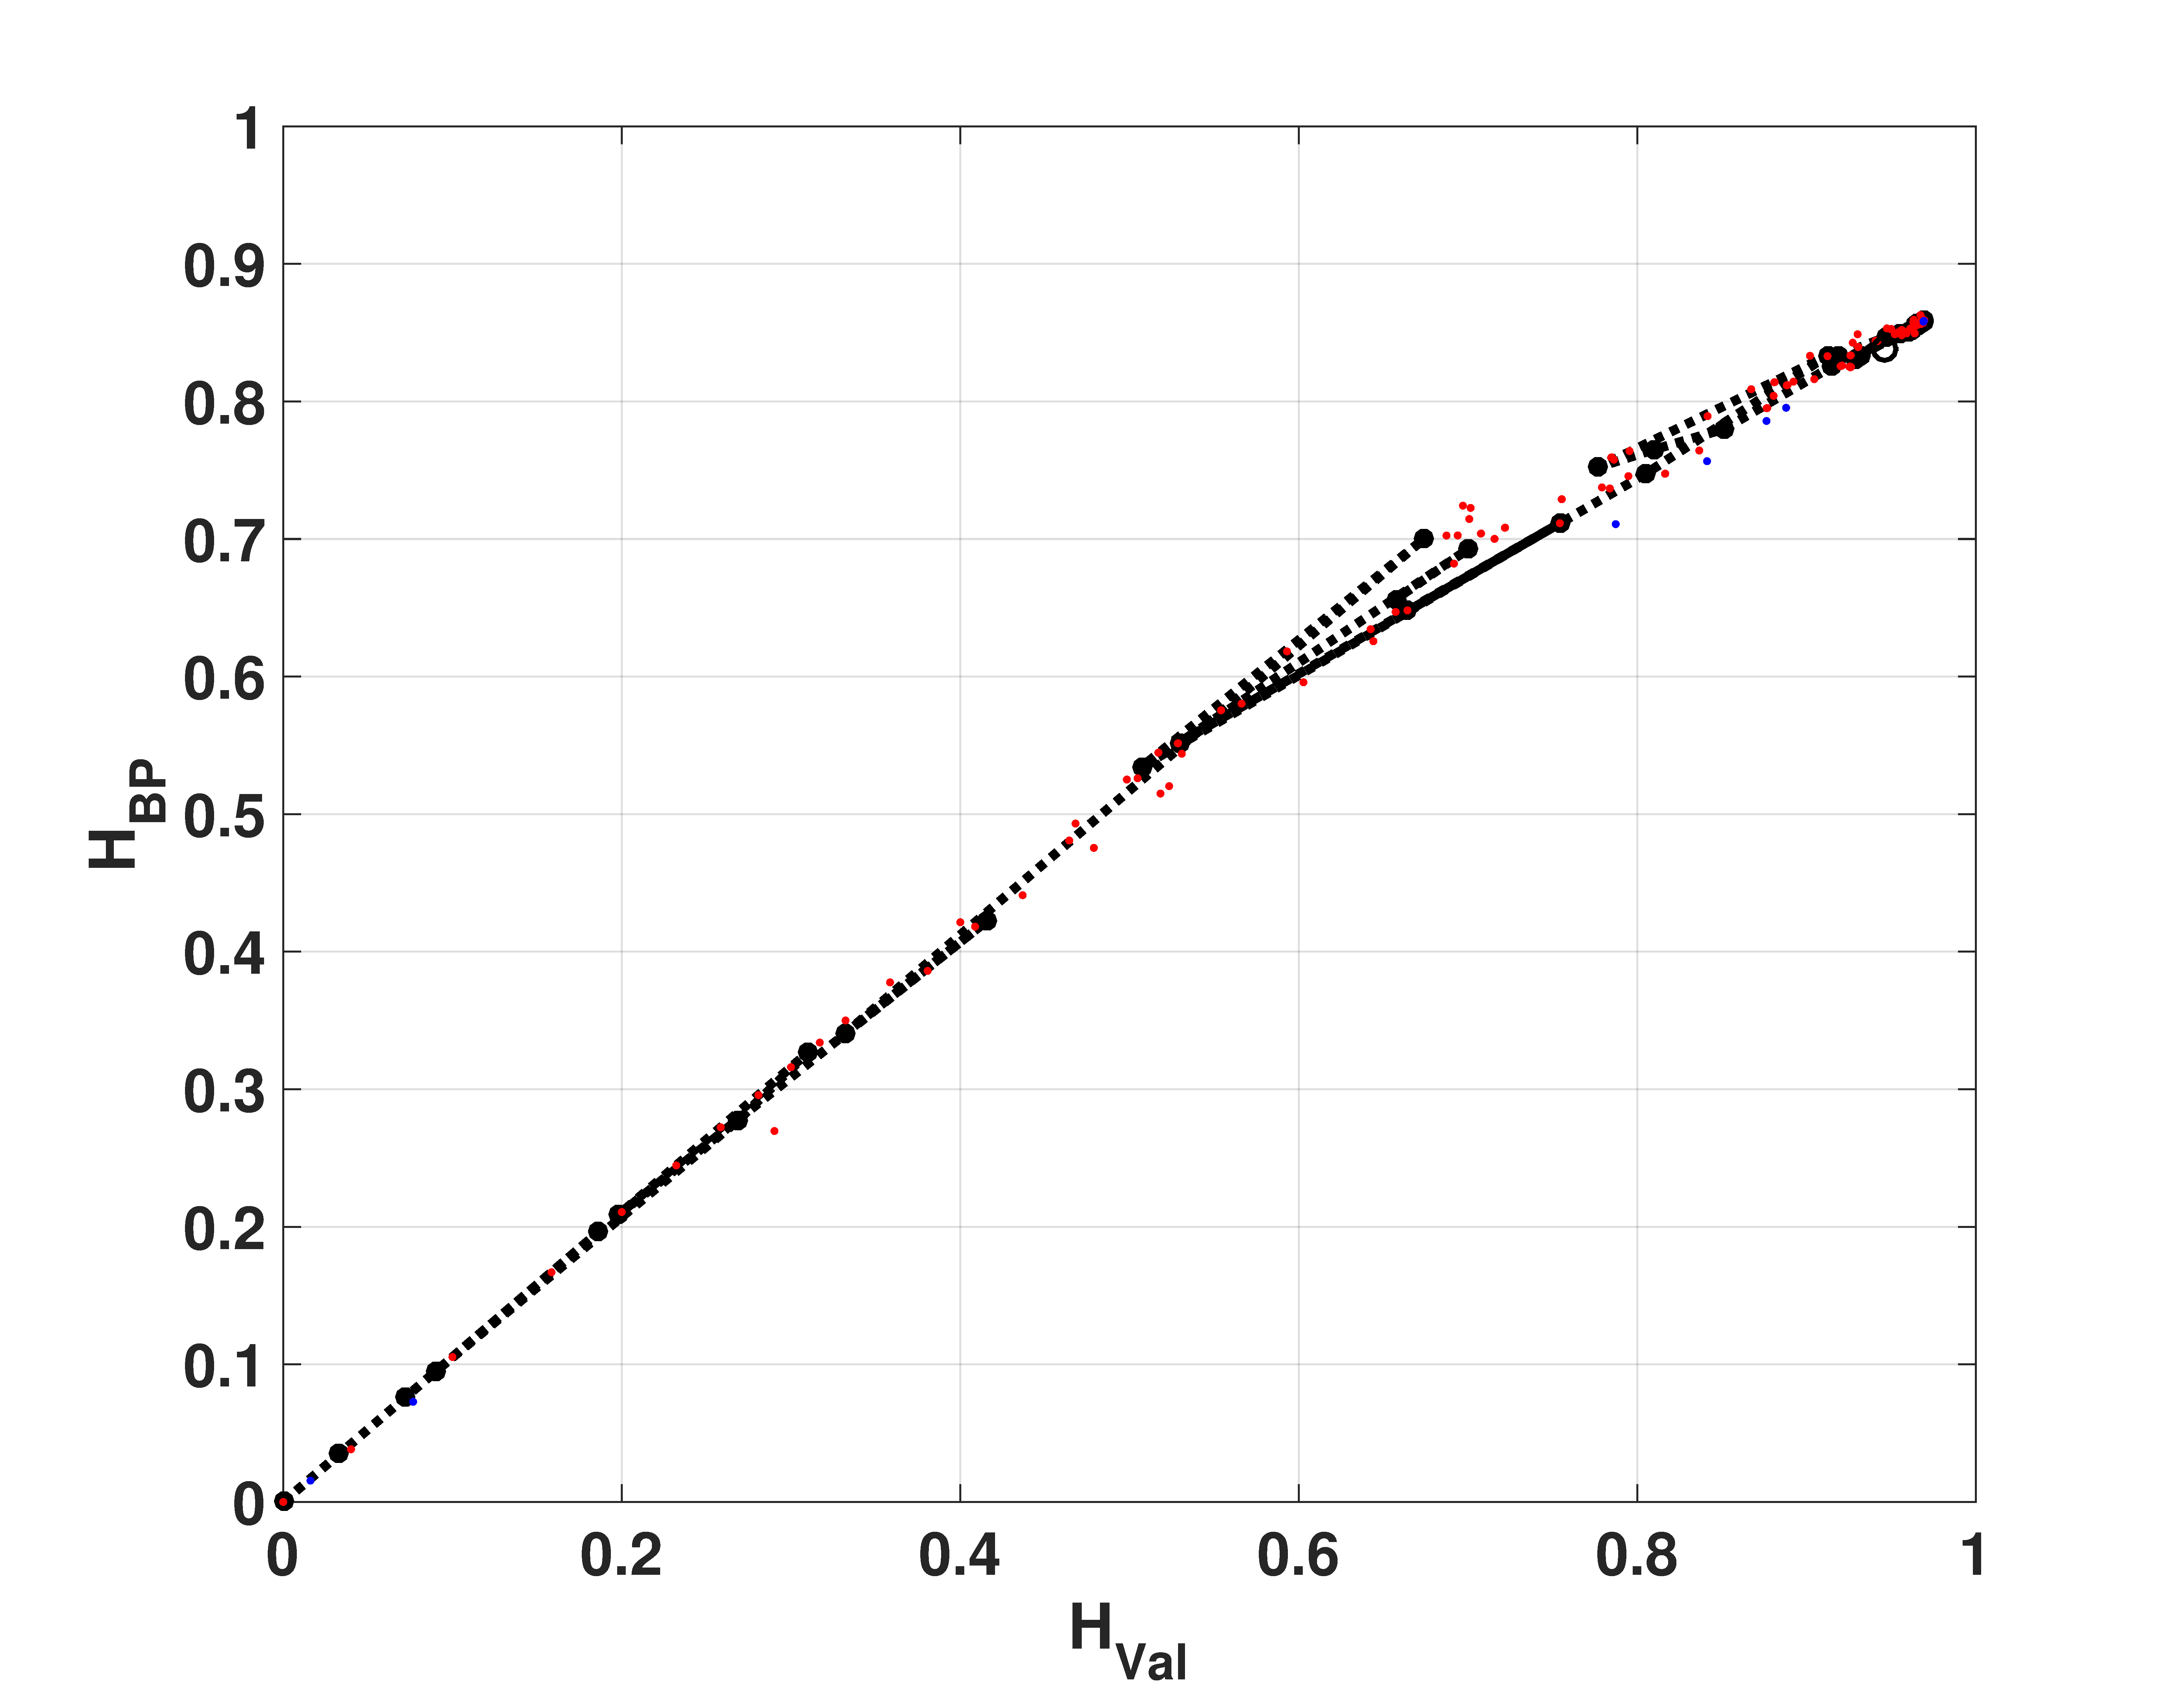
\includegraphics[width=.32\textwidth]{HbpHval_SwitchEven}
	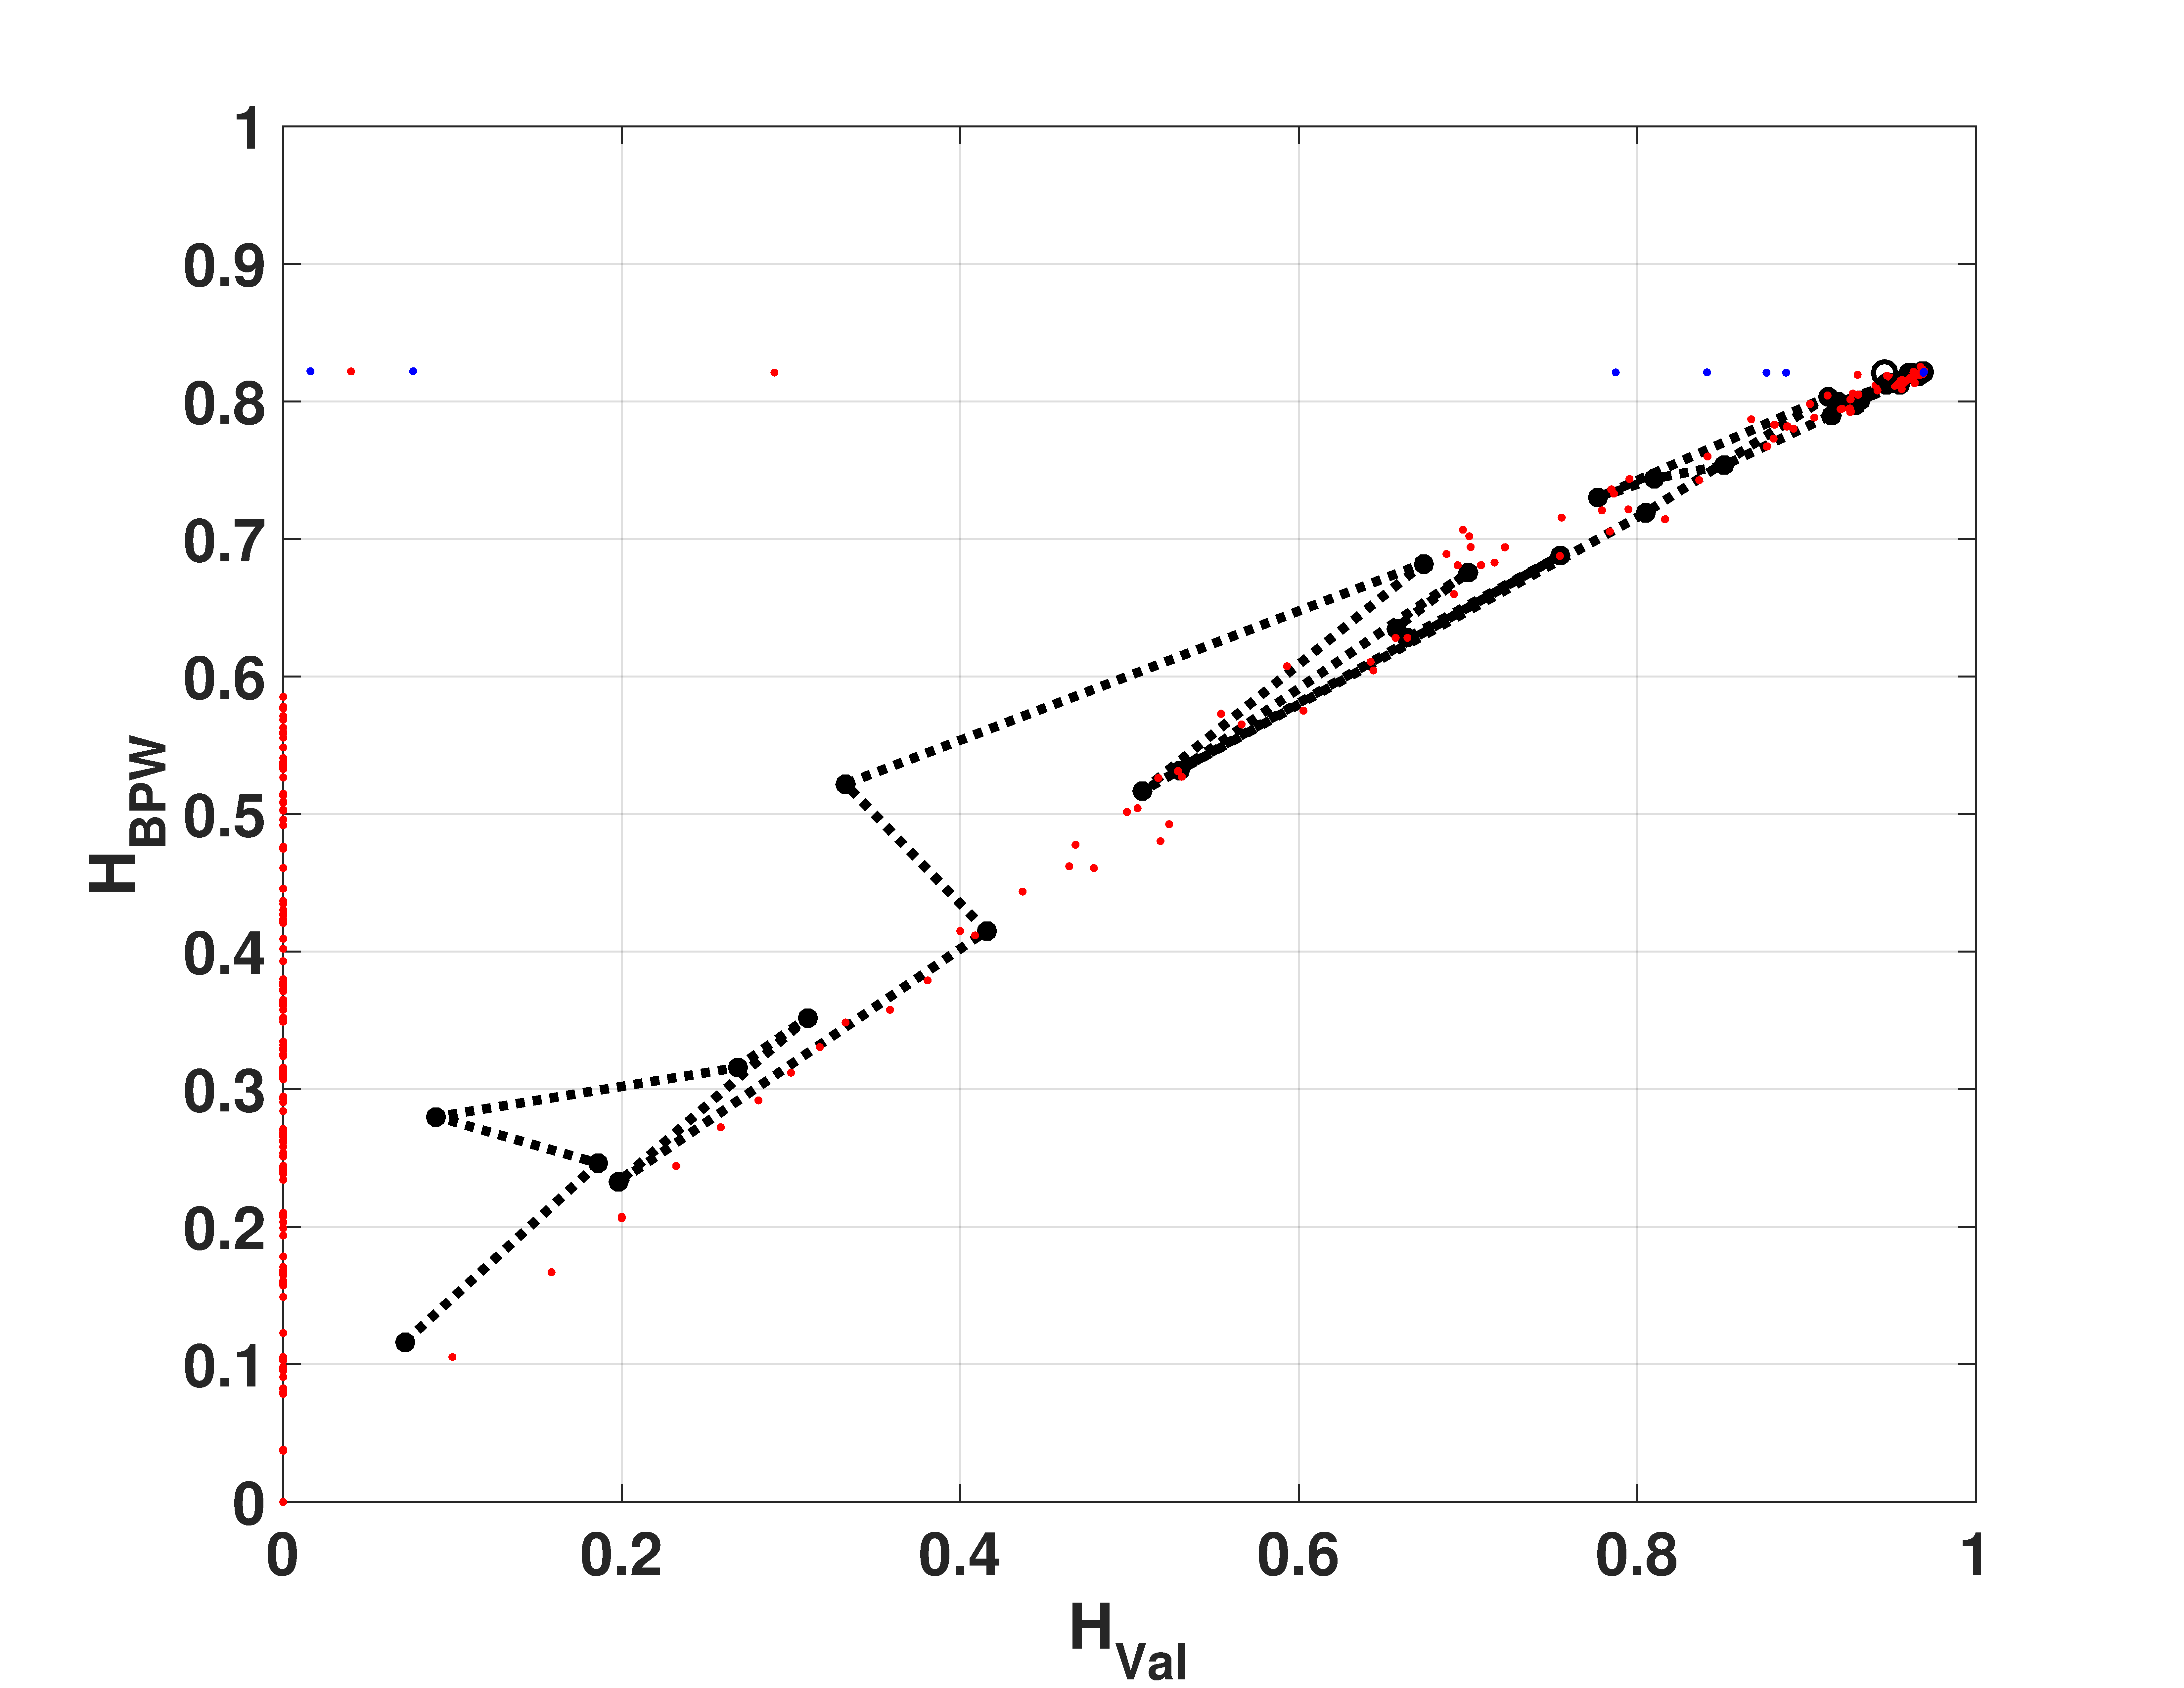
\includegraphics[width=.32\textwidth]{HbpwHval_SwitchEven}
	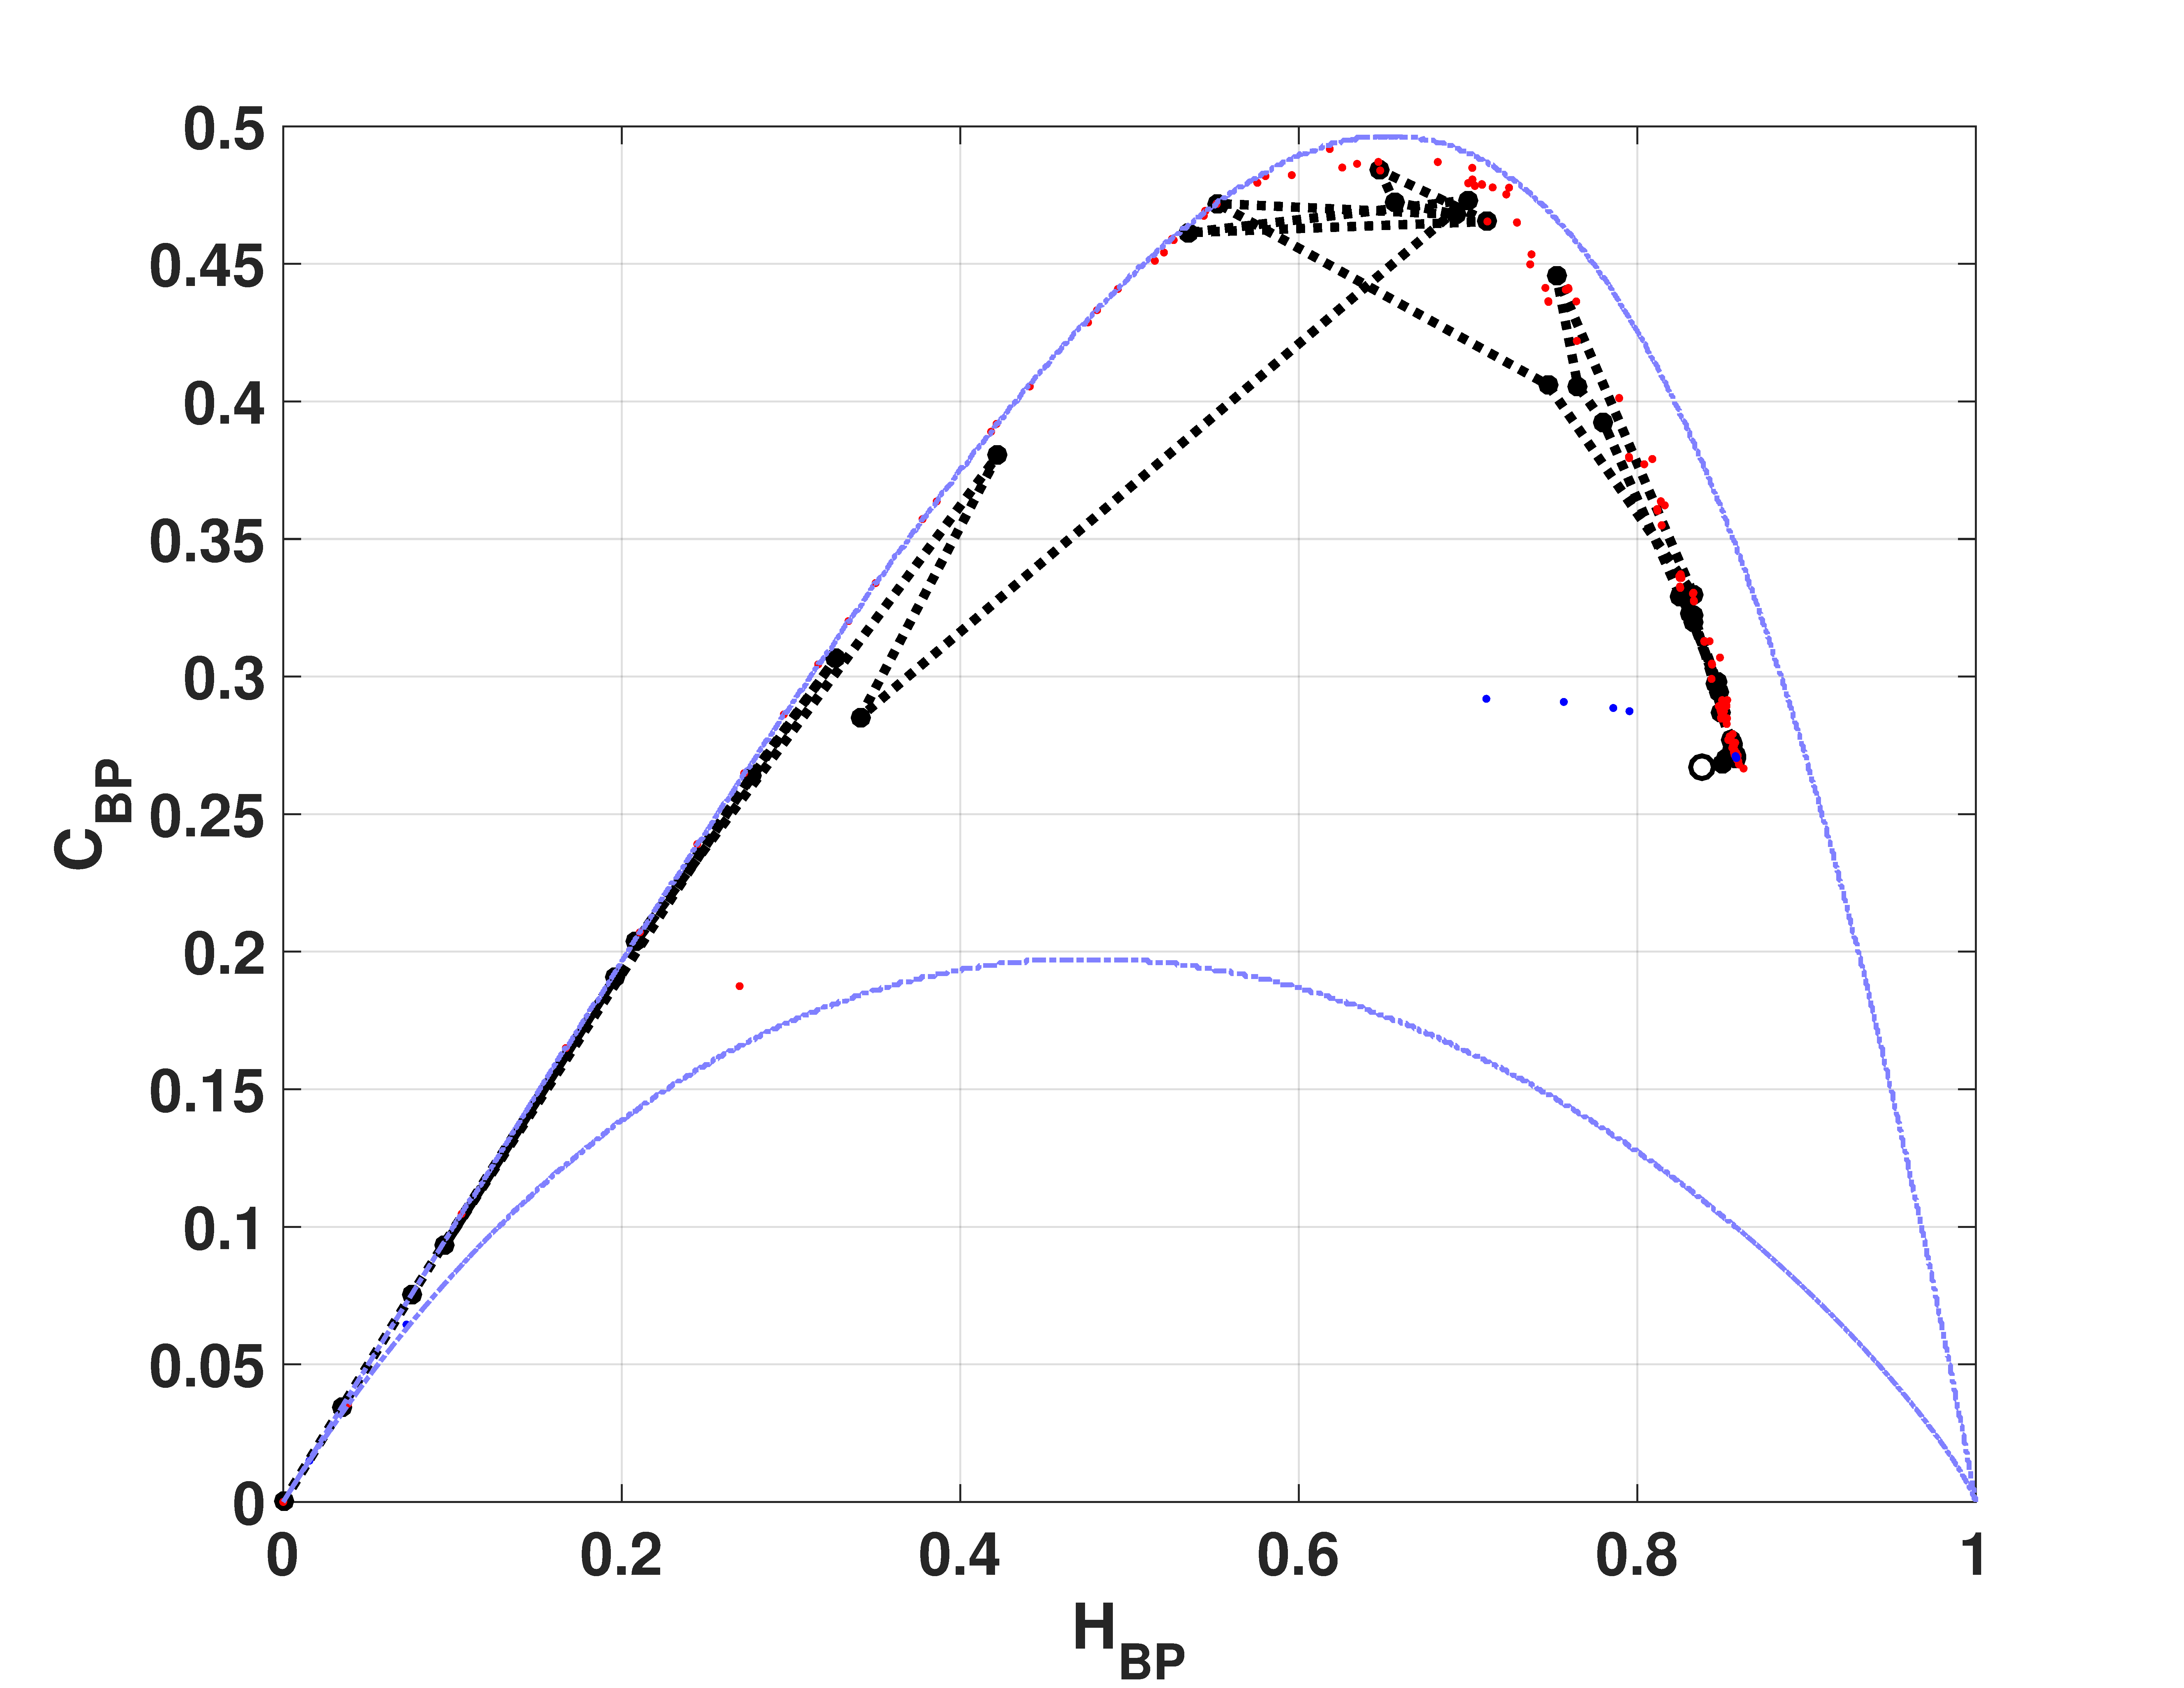
\includegraphics[width=.32\textwidth]{CbpHbp_SwitchEven}
	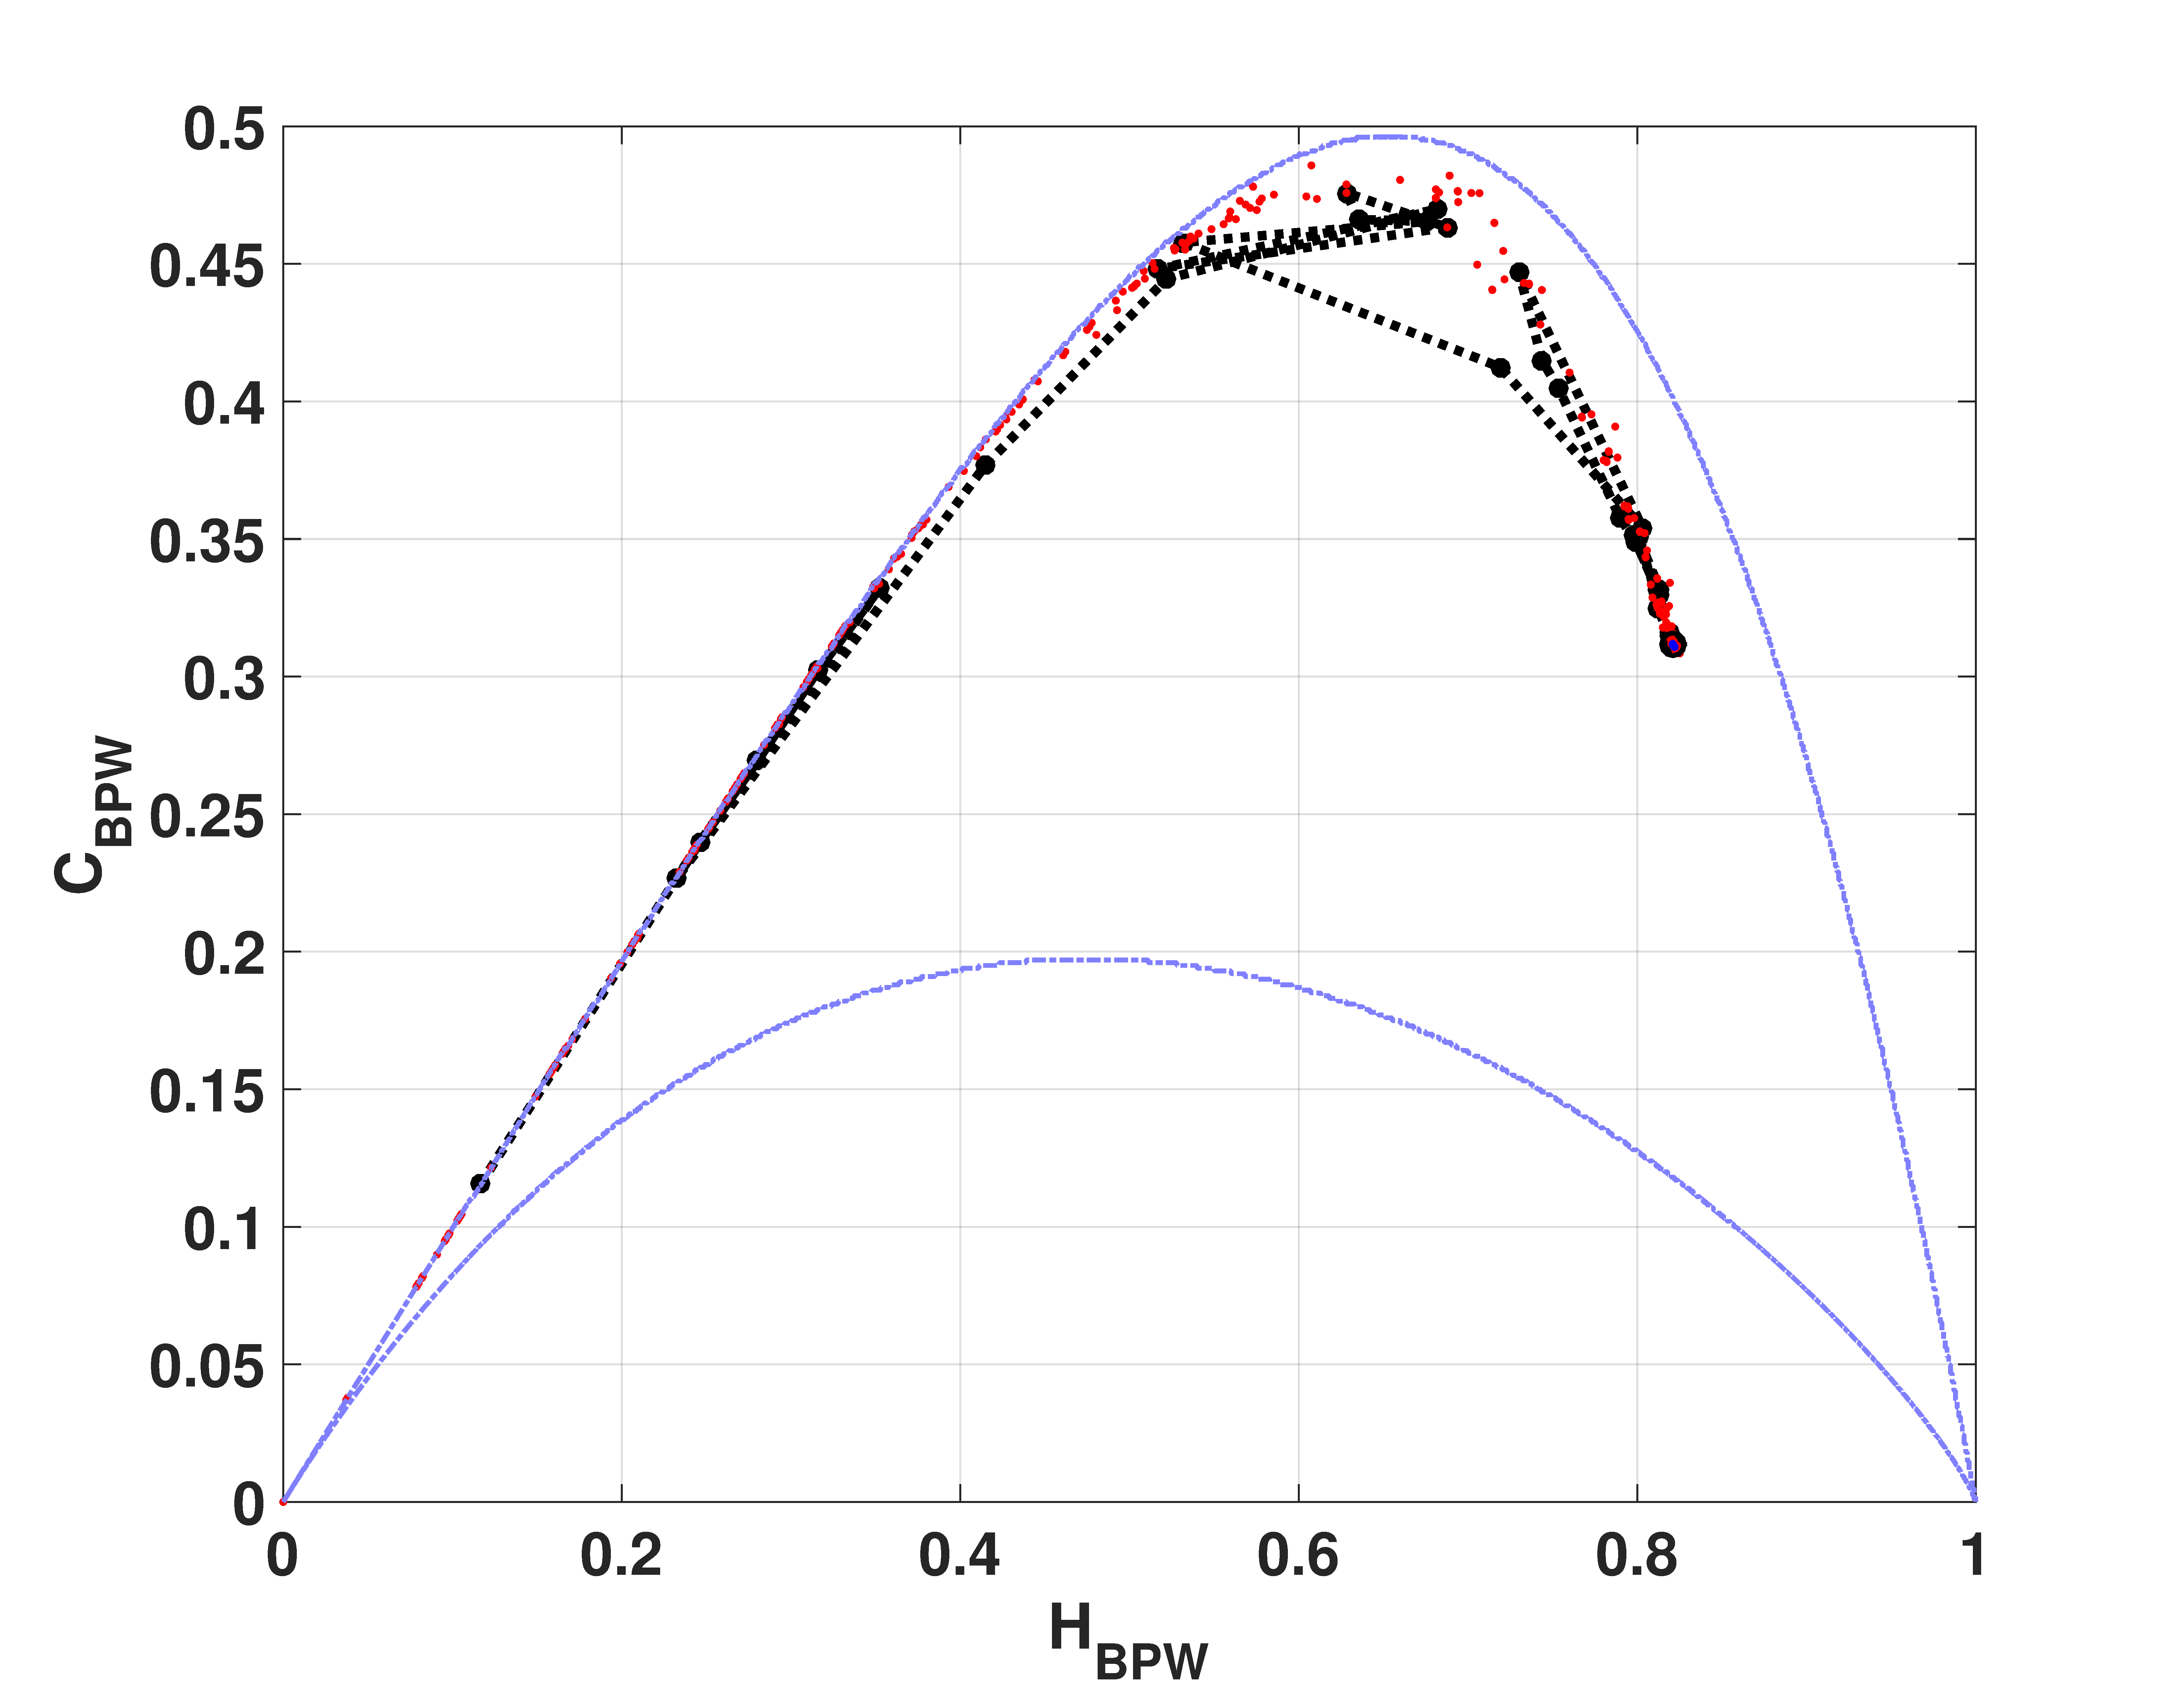
\includegraphics[width=.32\textwidth]{CbpwHbpw_SwitchEven}
	\caption{Statistical properties of EVEN, obtained by skipping the values in the odd position of the time series of  SWITCH,  using binary representation: (a) $H_{hist}$ vs $P$ (b) $H_{BP}$ vs $P$ (c) $C_{BP}$ vs $P$ (d) Number of missing ordering patterns $MP$ vs $P$. In Figures (a) to (d) dashed line correspond to floating point numbers. (e) representation in the $H_{hist},H_{BP}$ plane in the the binary numerical system.  The star represents the state for floating points numbers. (f) representation in the $H_{BP},C_{BP}$ plane.  The star represents the state for floating points numbers.  } \label{fig:seqimparbin}
\end{figure}


\begin{figure}
	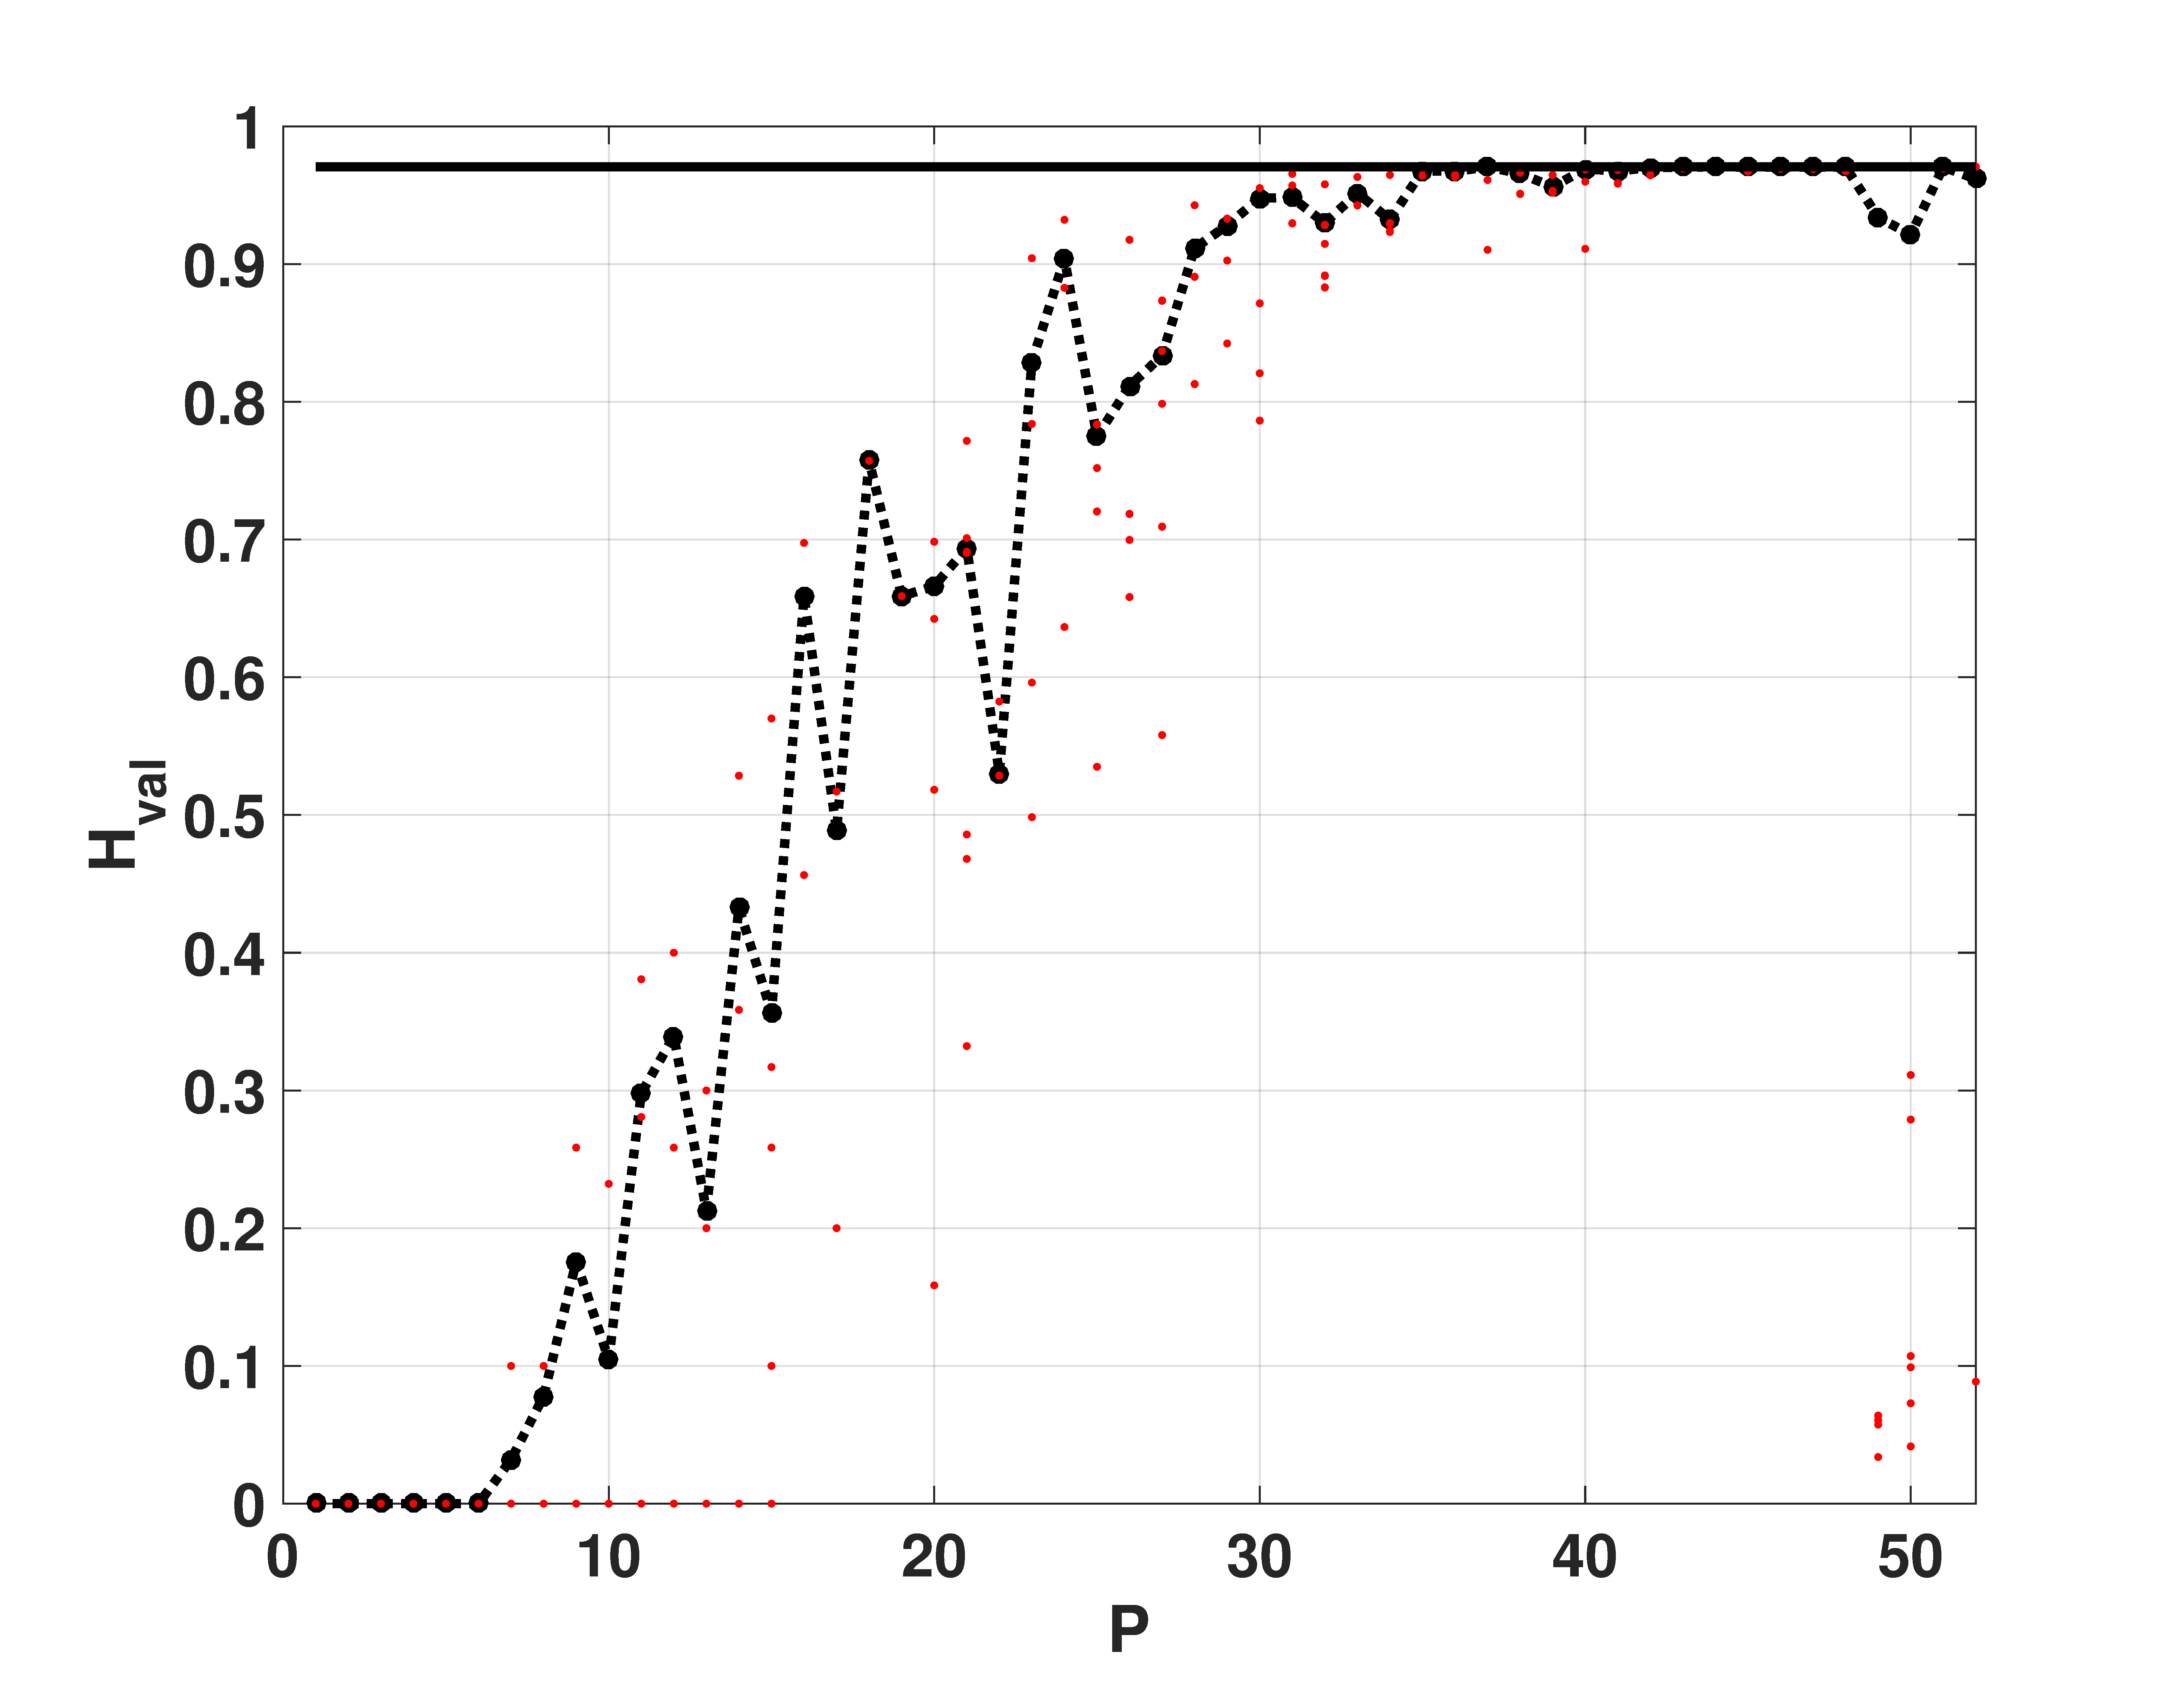
\includegraphics[width=.32\textwidth]{Hval_SwitchOdd}
	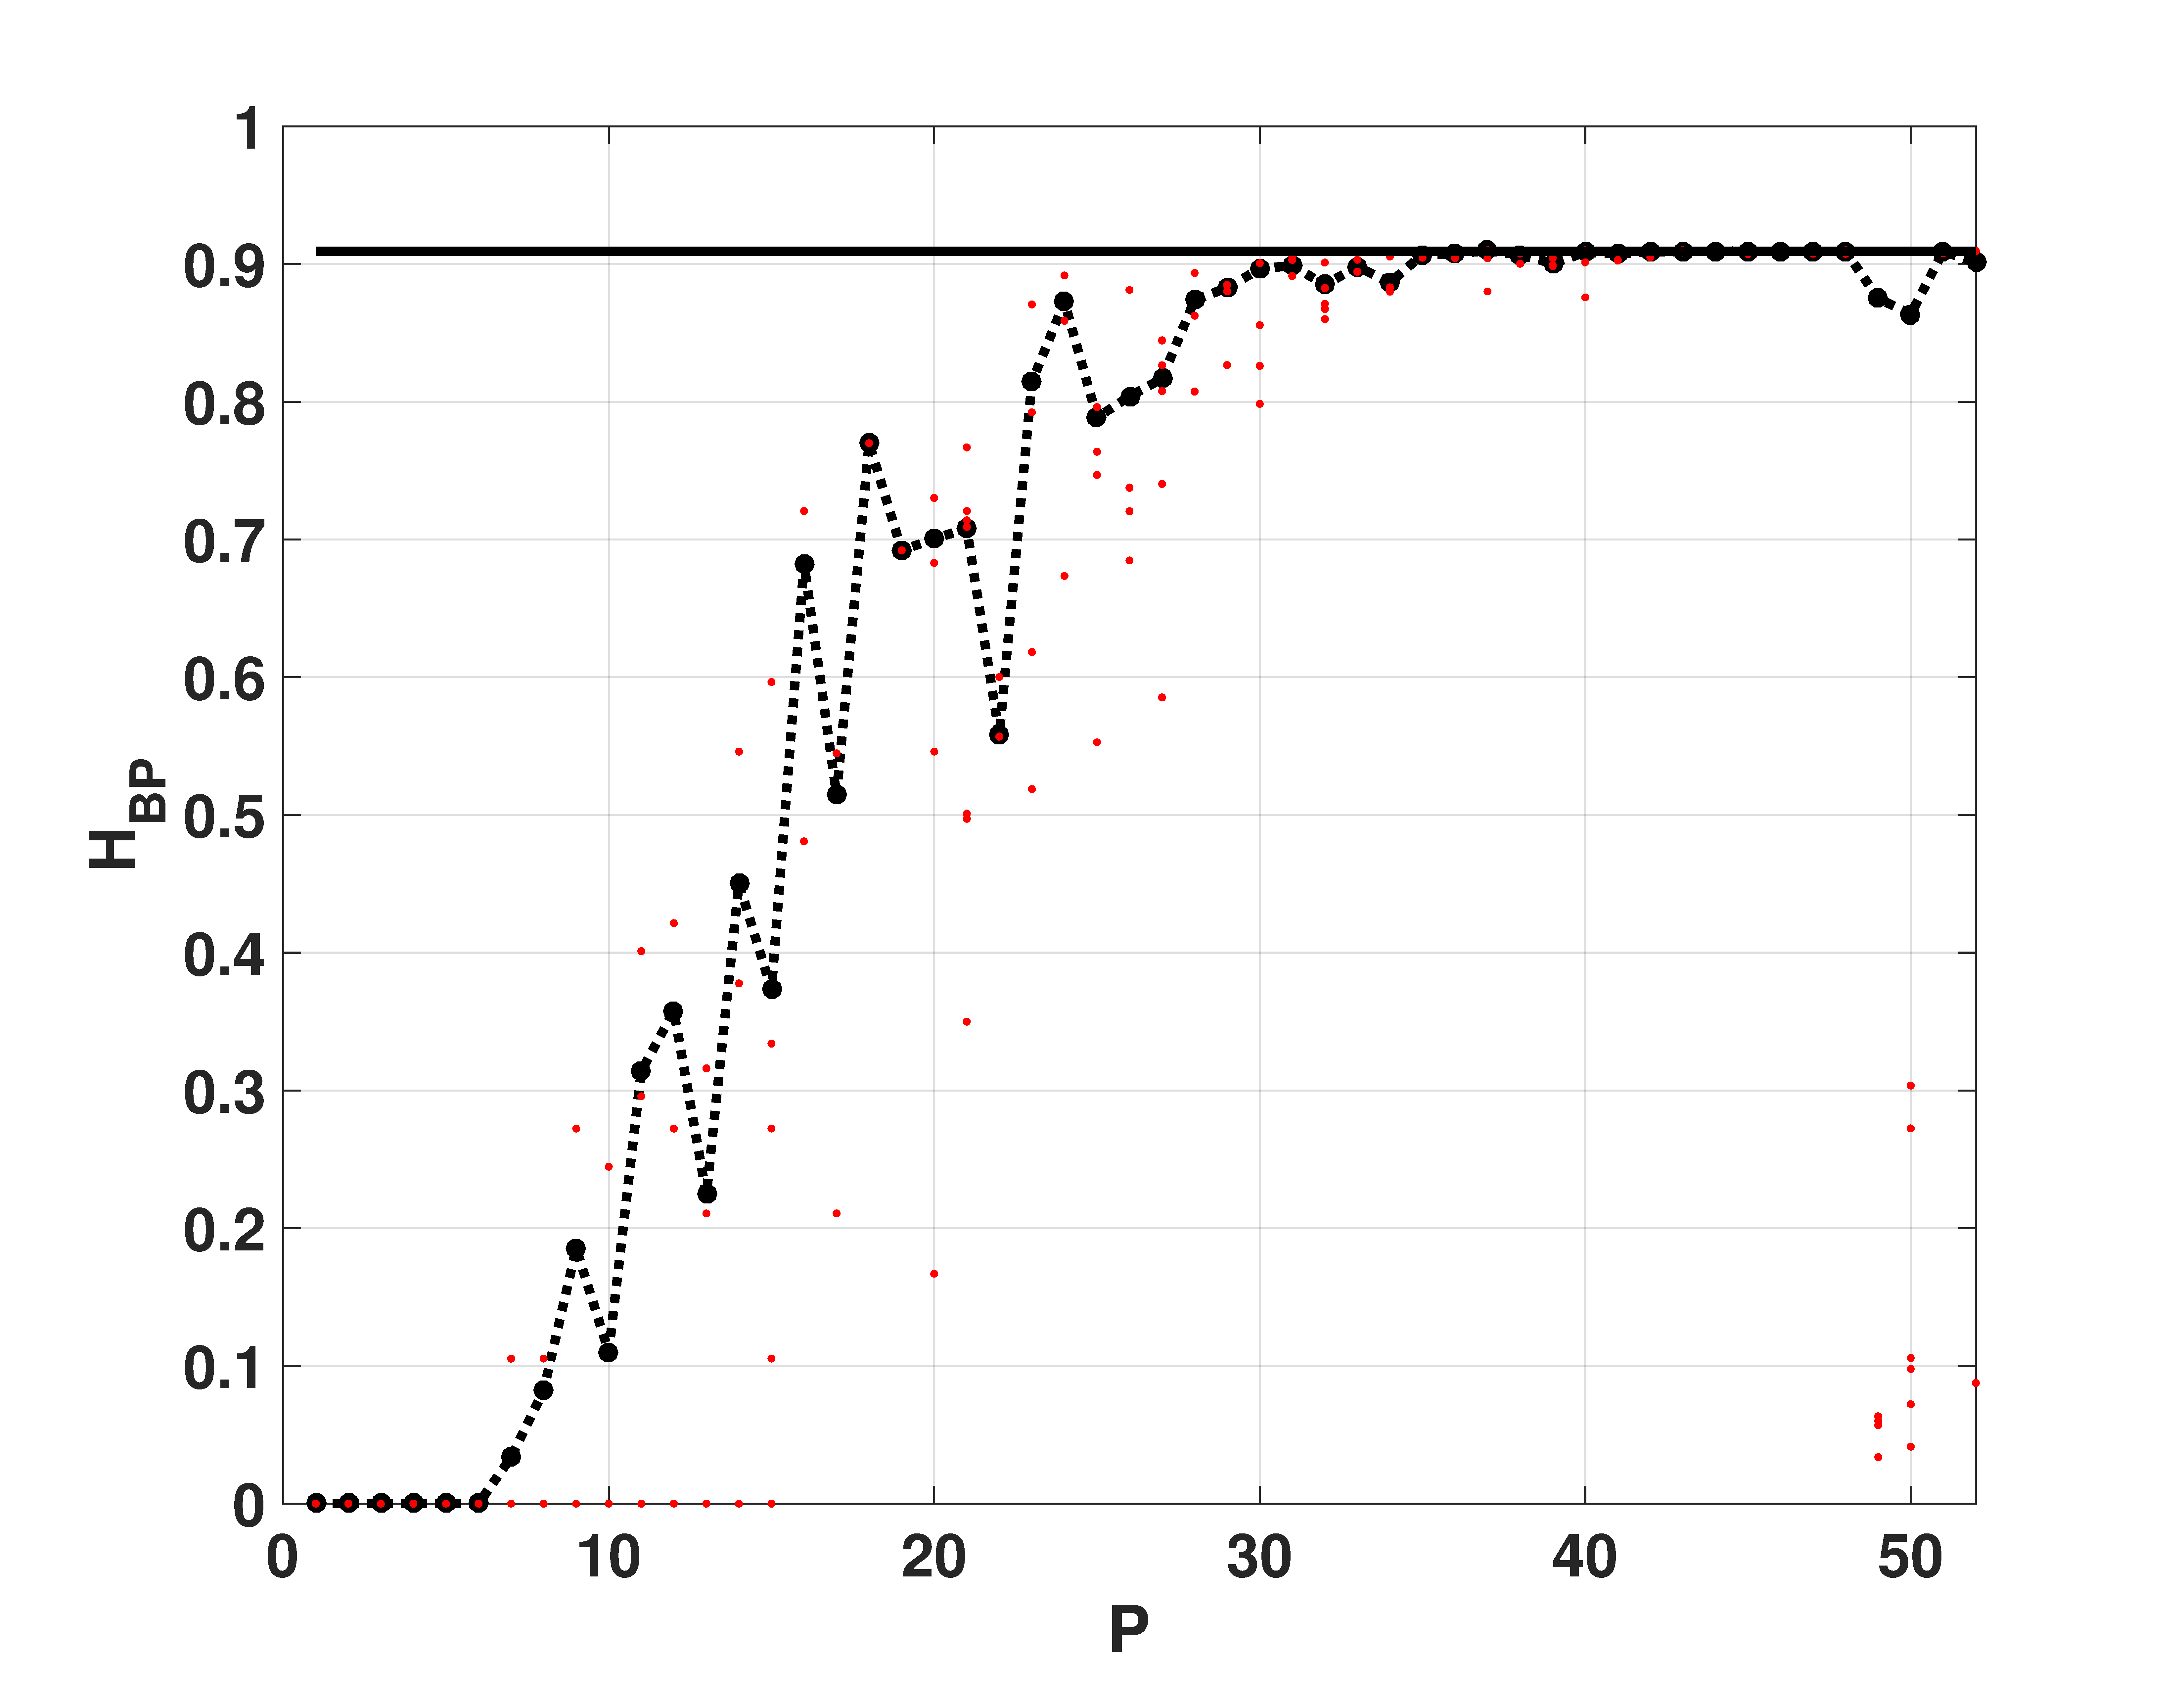
\includegraphics[width=.32\textwidth]{Hbp_SwitchOdd}
	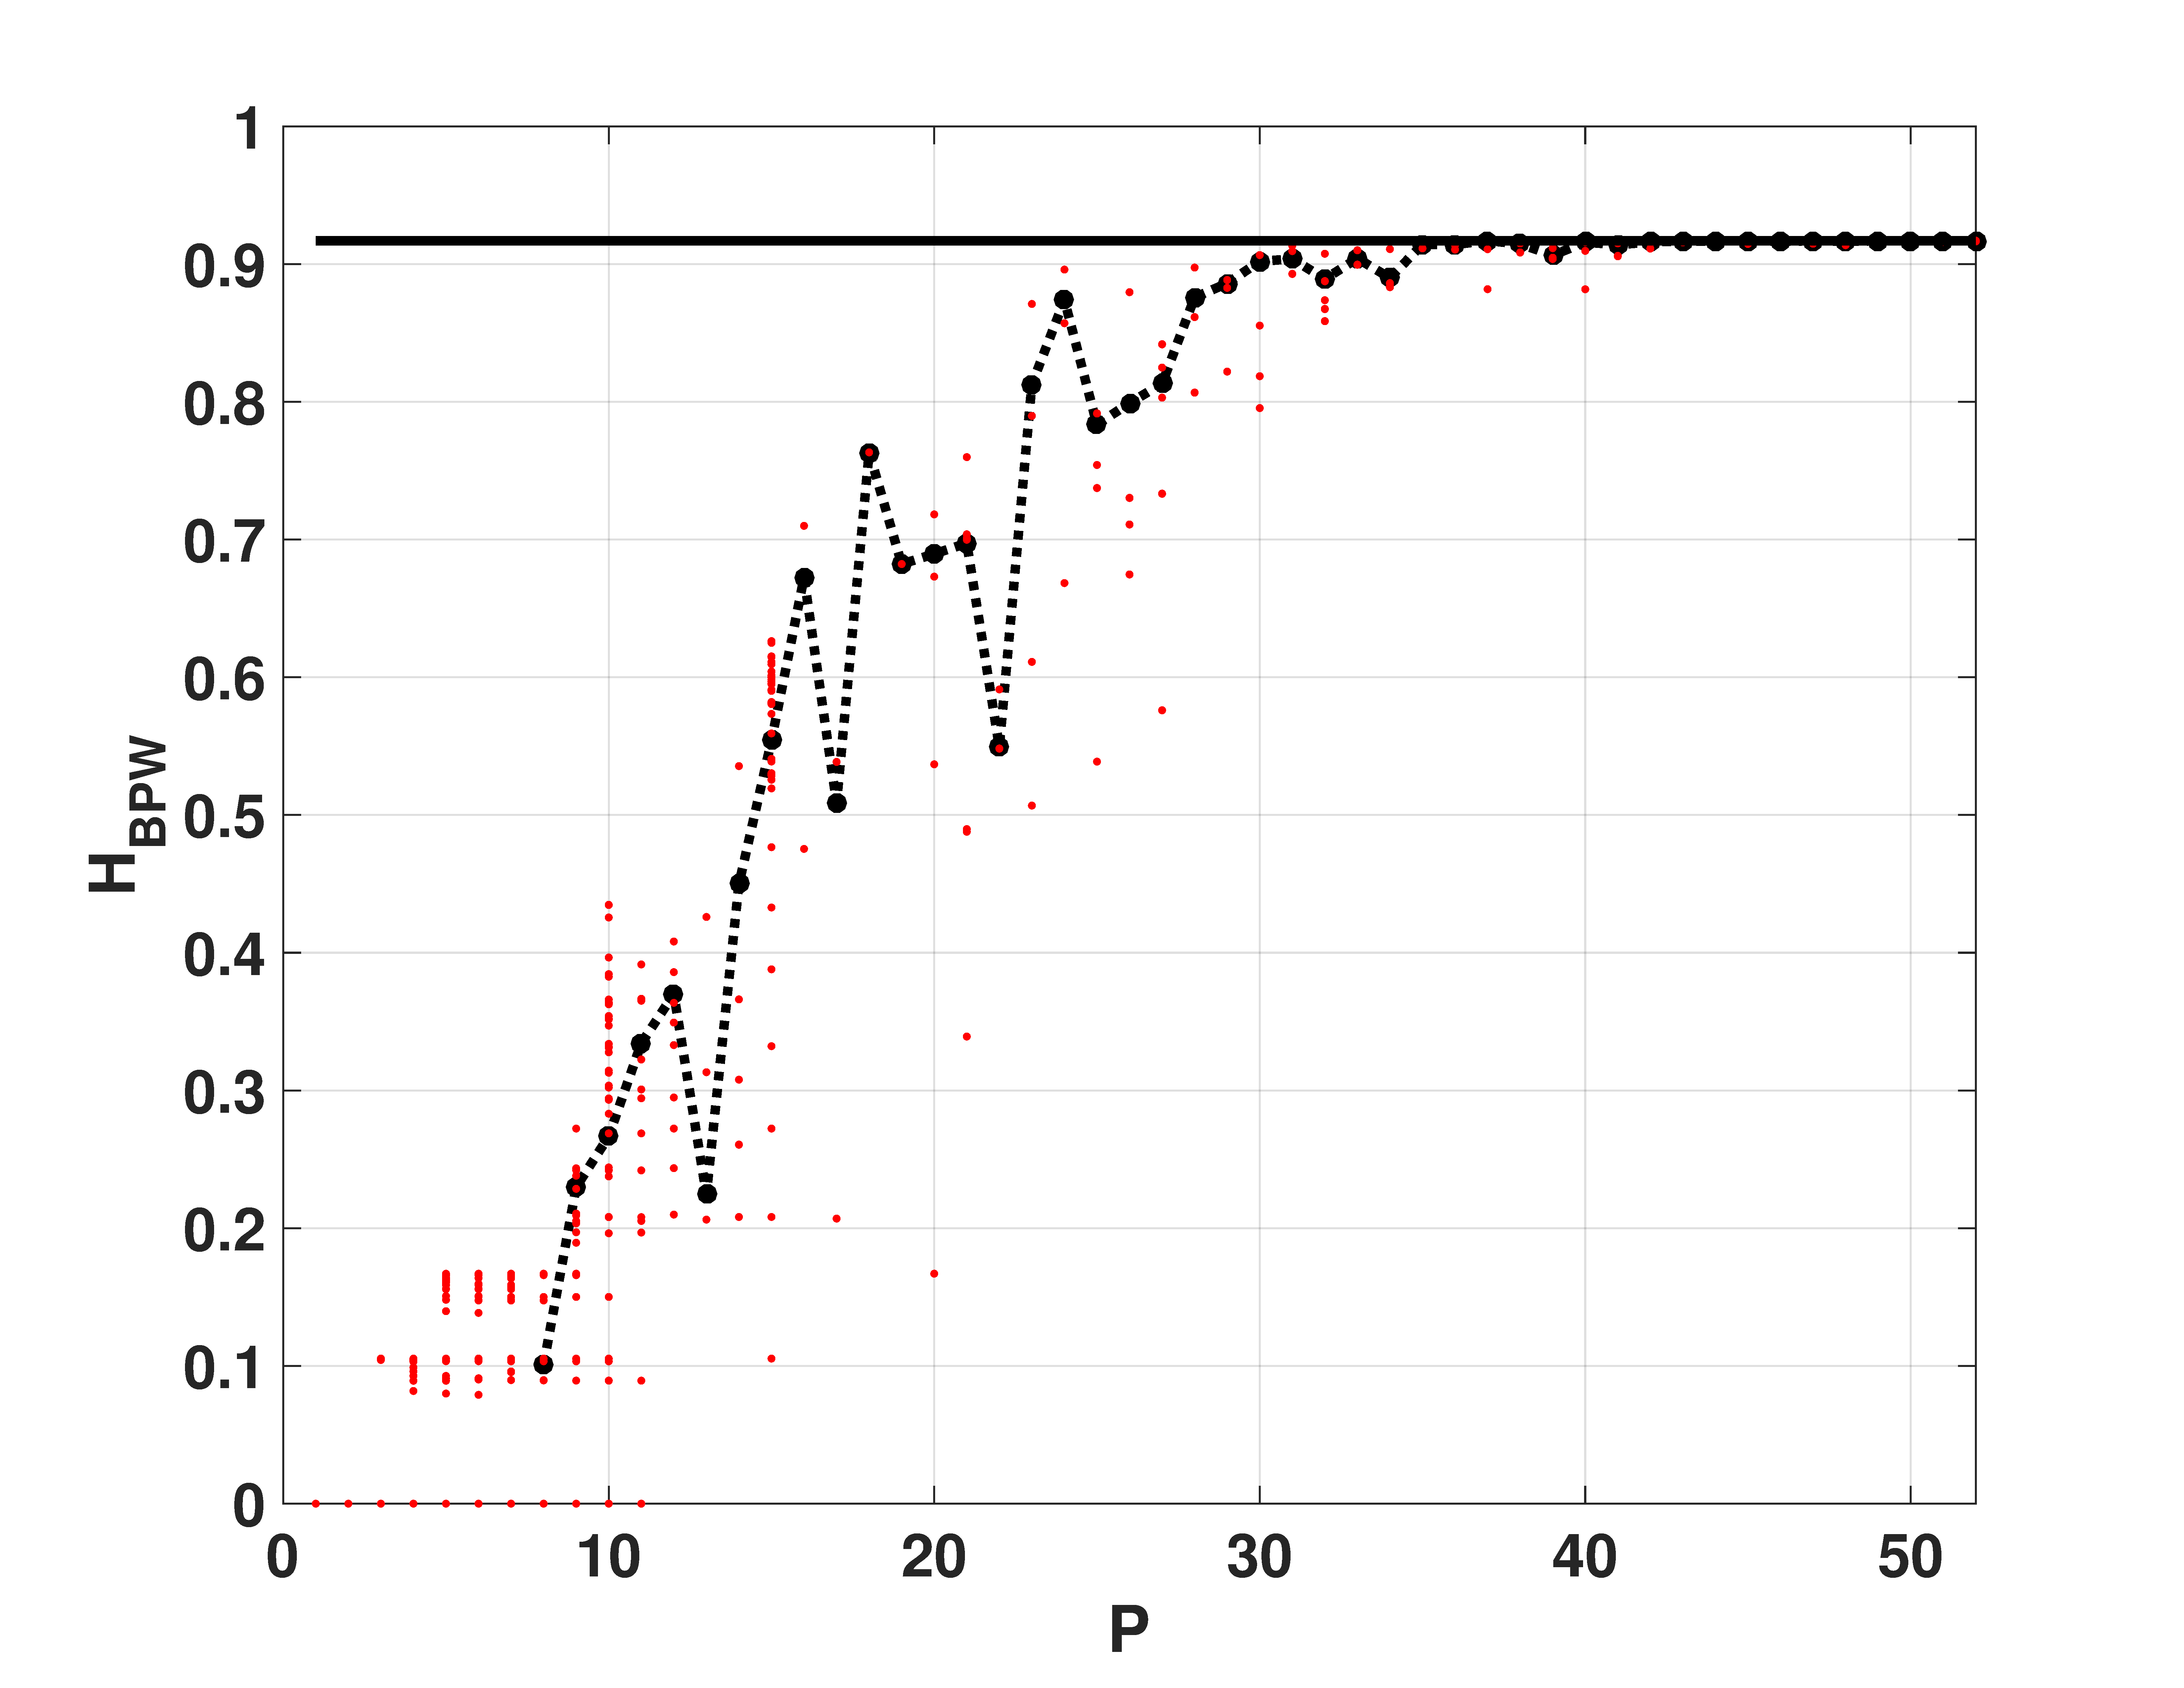
\includegraphics[width=.32\textwidth]{Hbpw_SwitchOdd}
	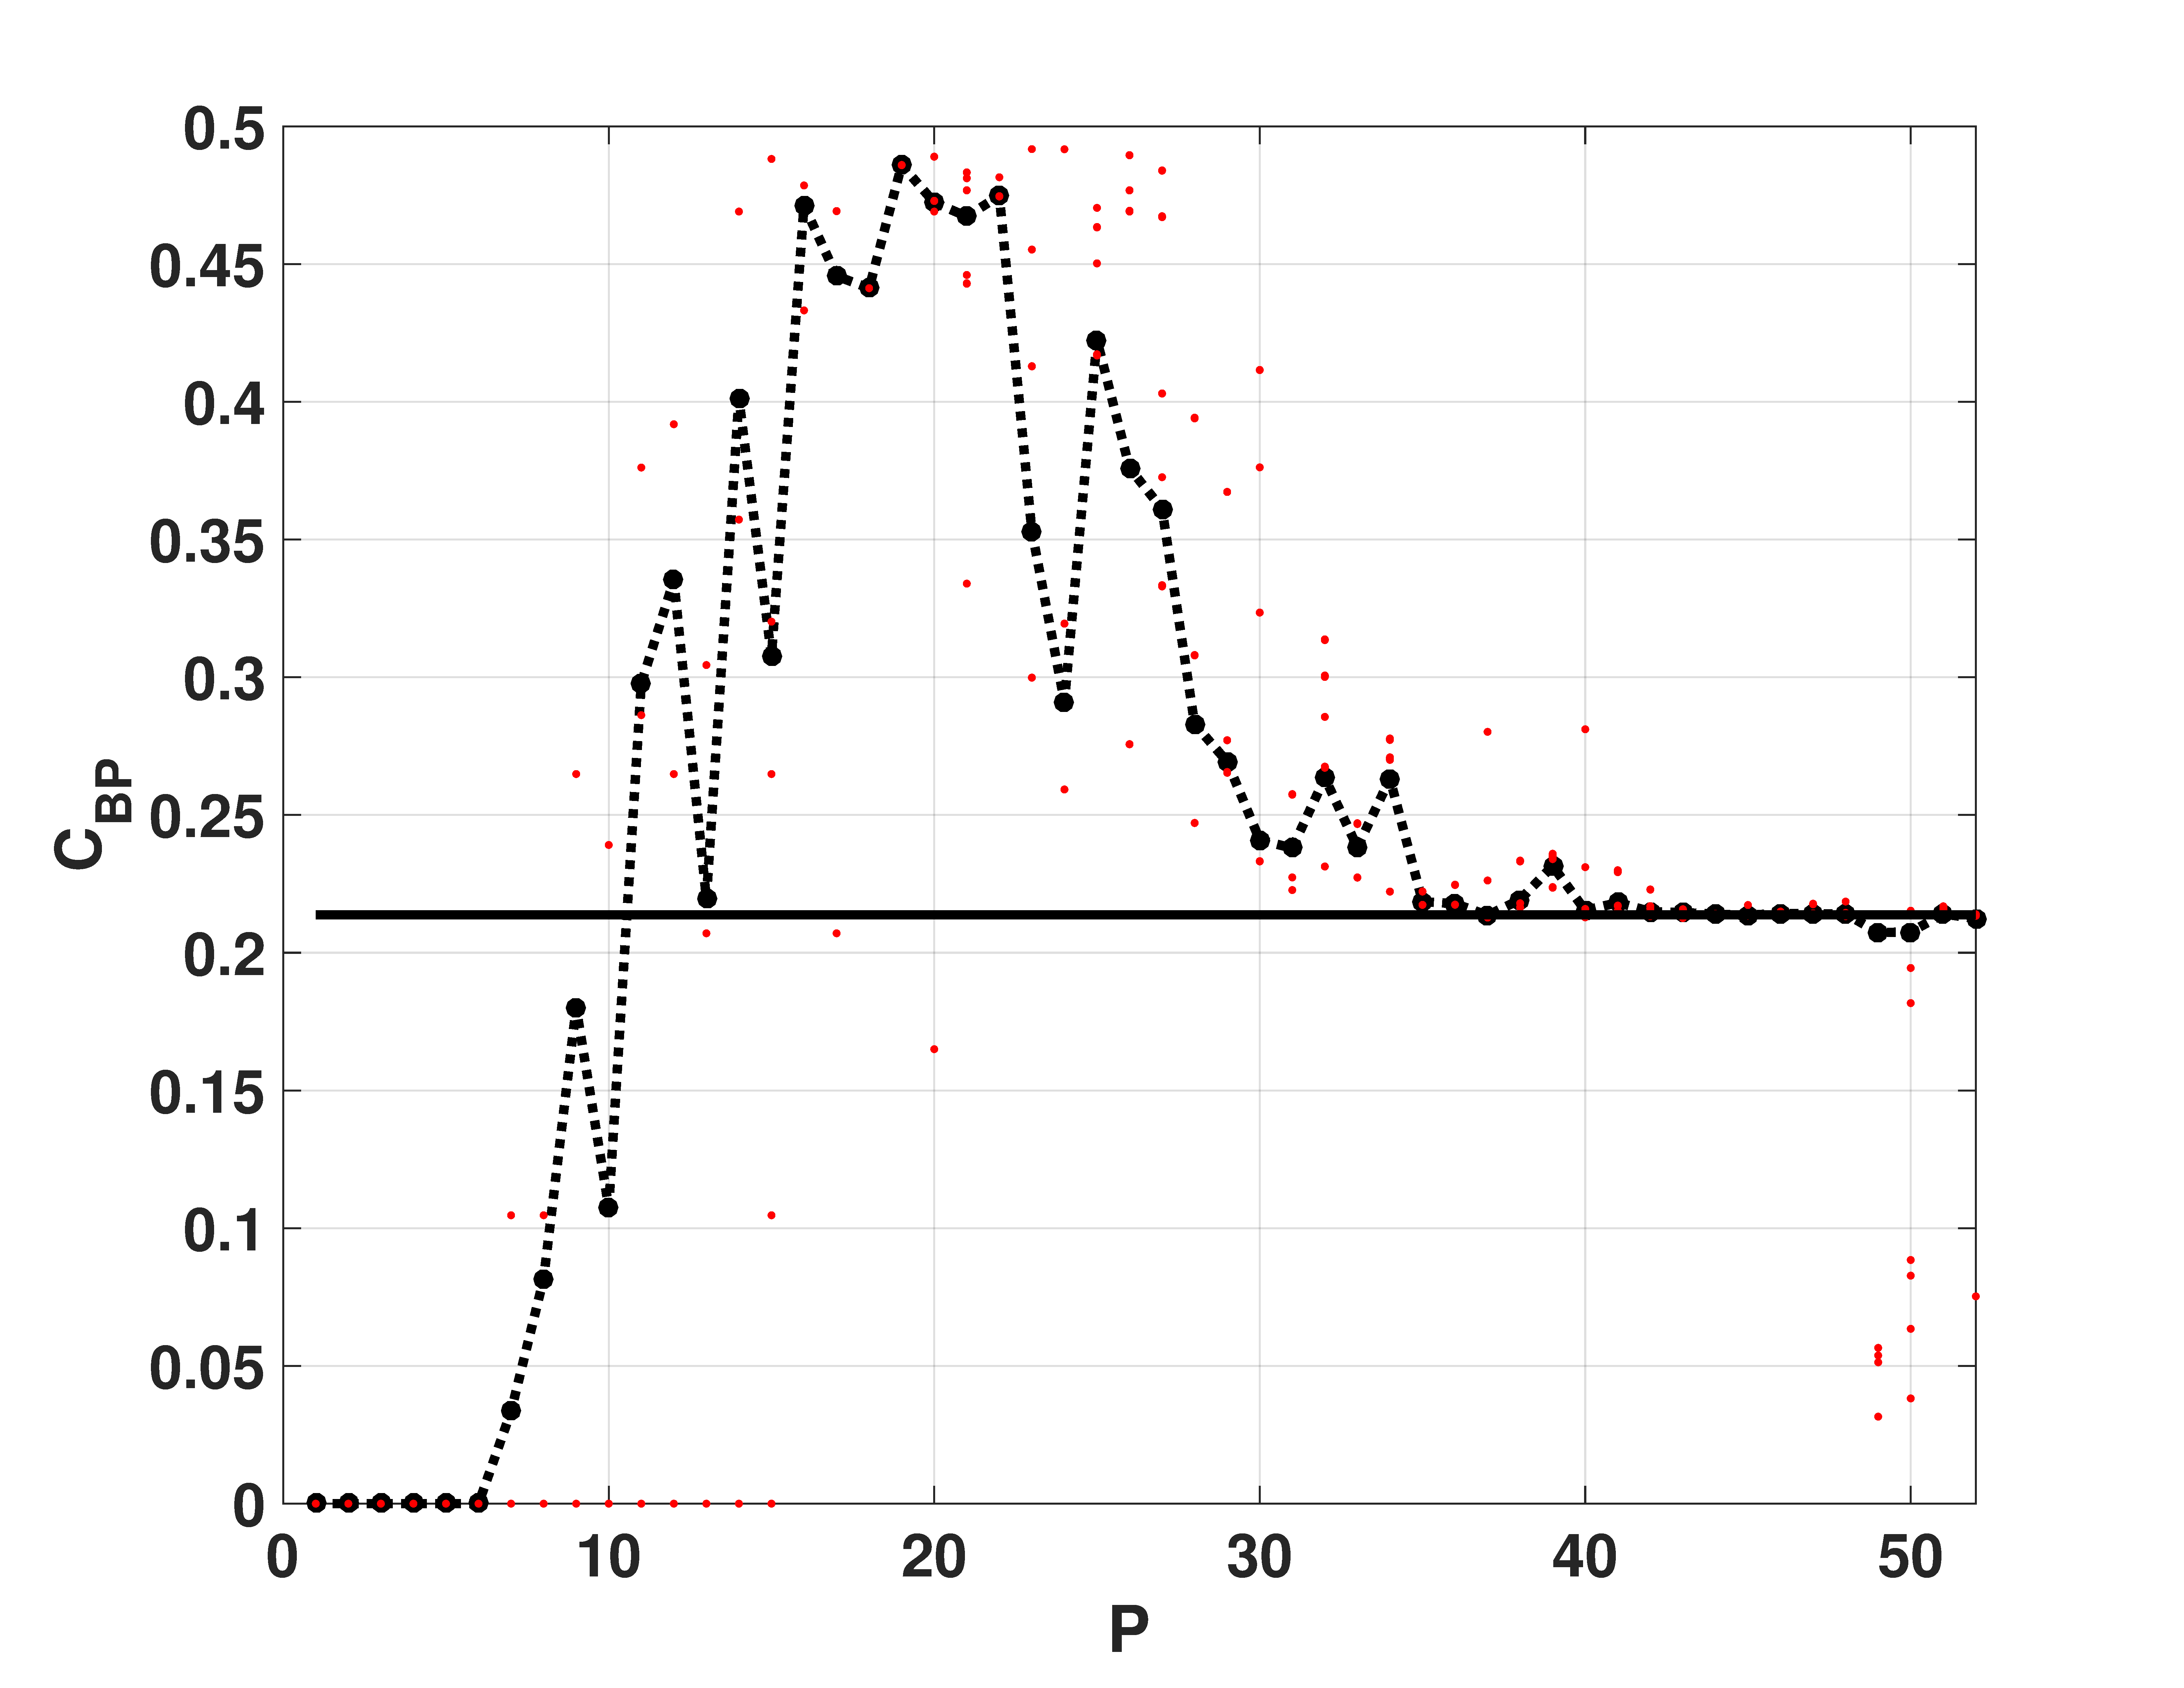
\includegraphics[width=.32\textwidth]{Cbp_SwitchOdd}
	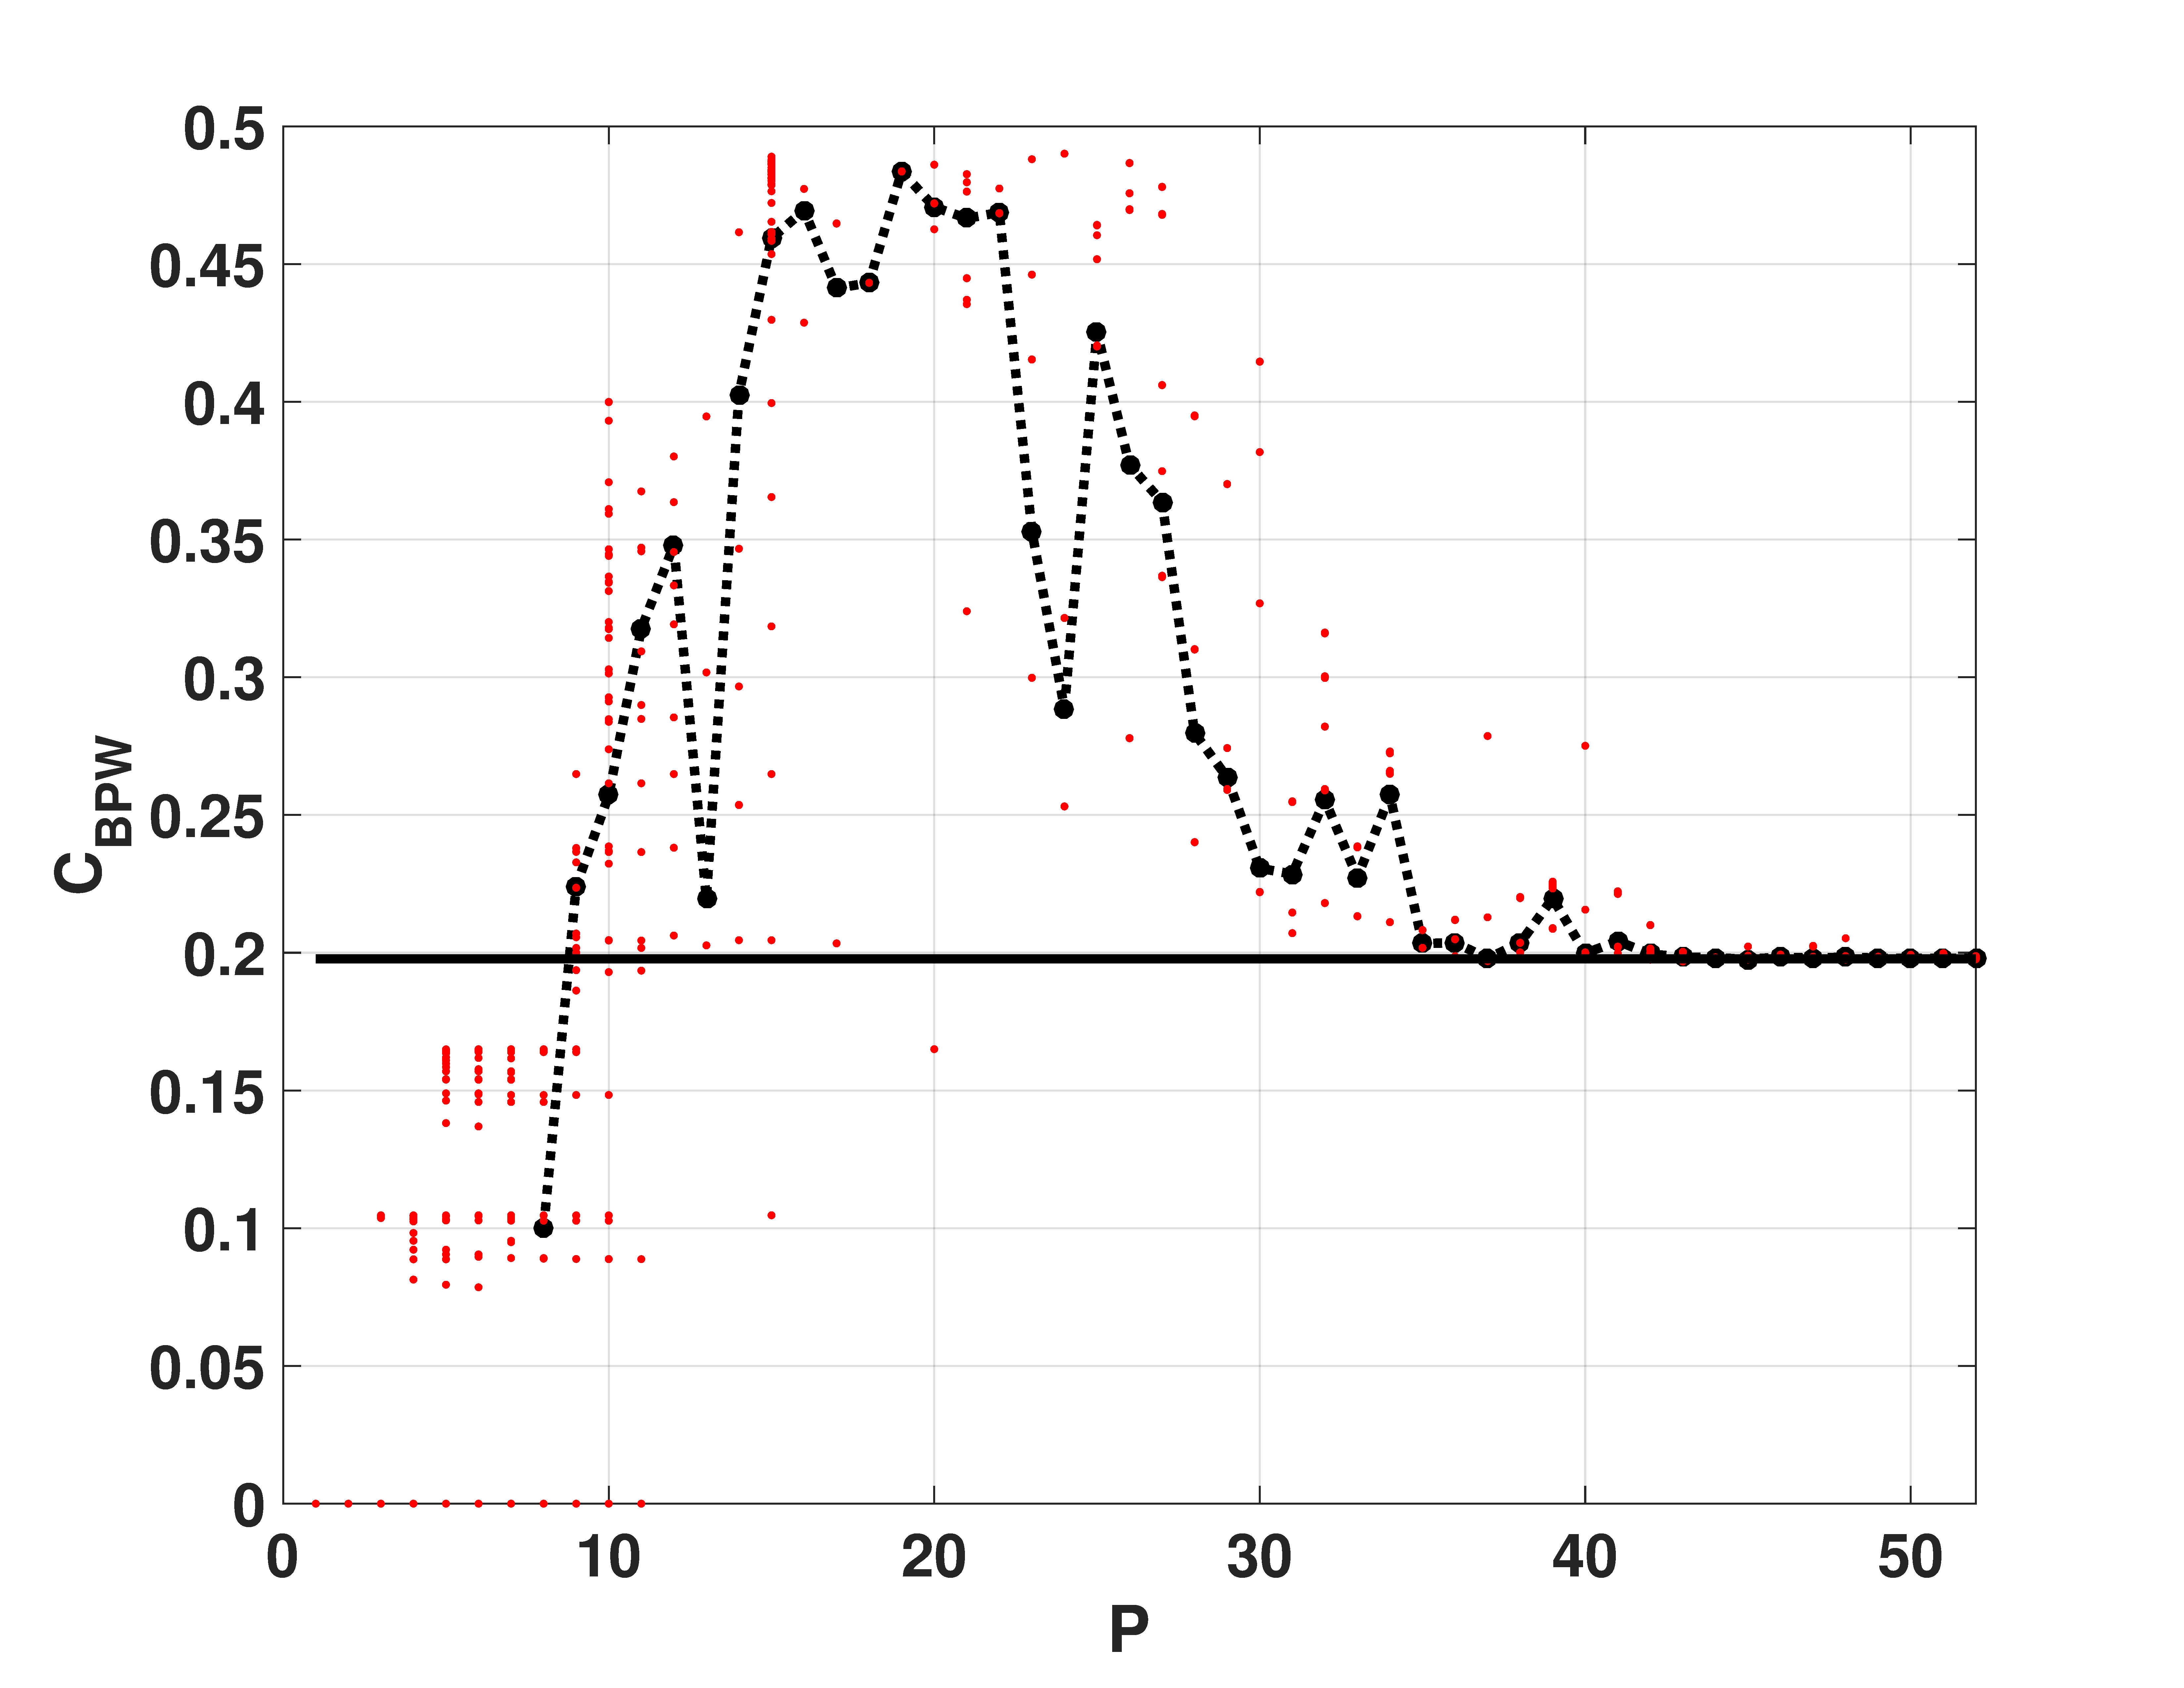
\includegraphics[width=.32\textwidth]{Cbpw_SwitchOdd}
	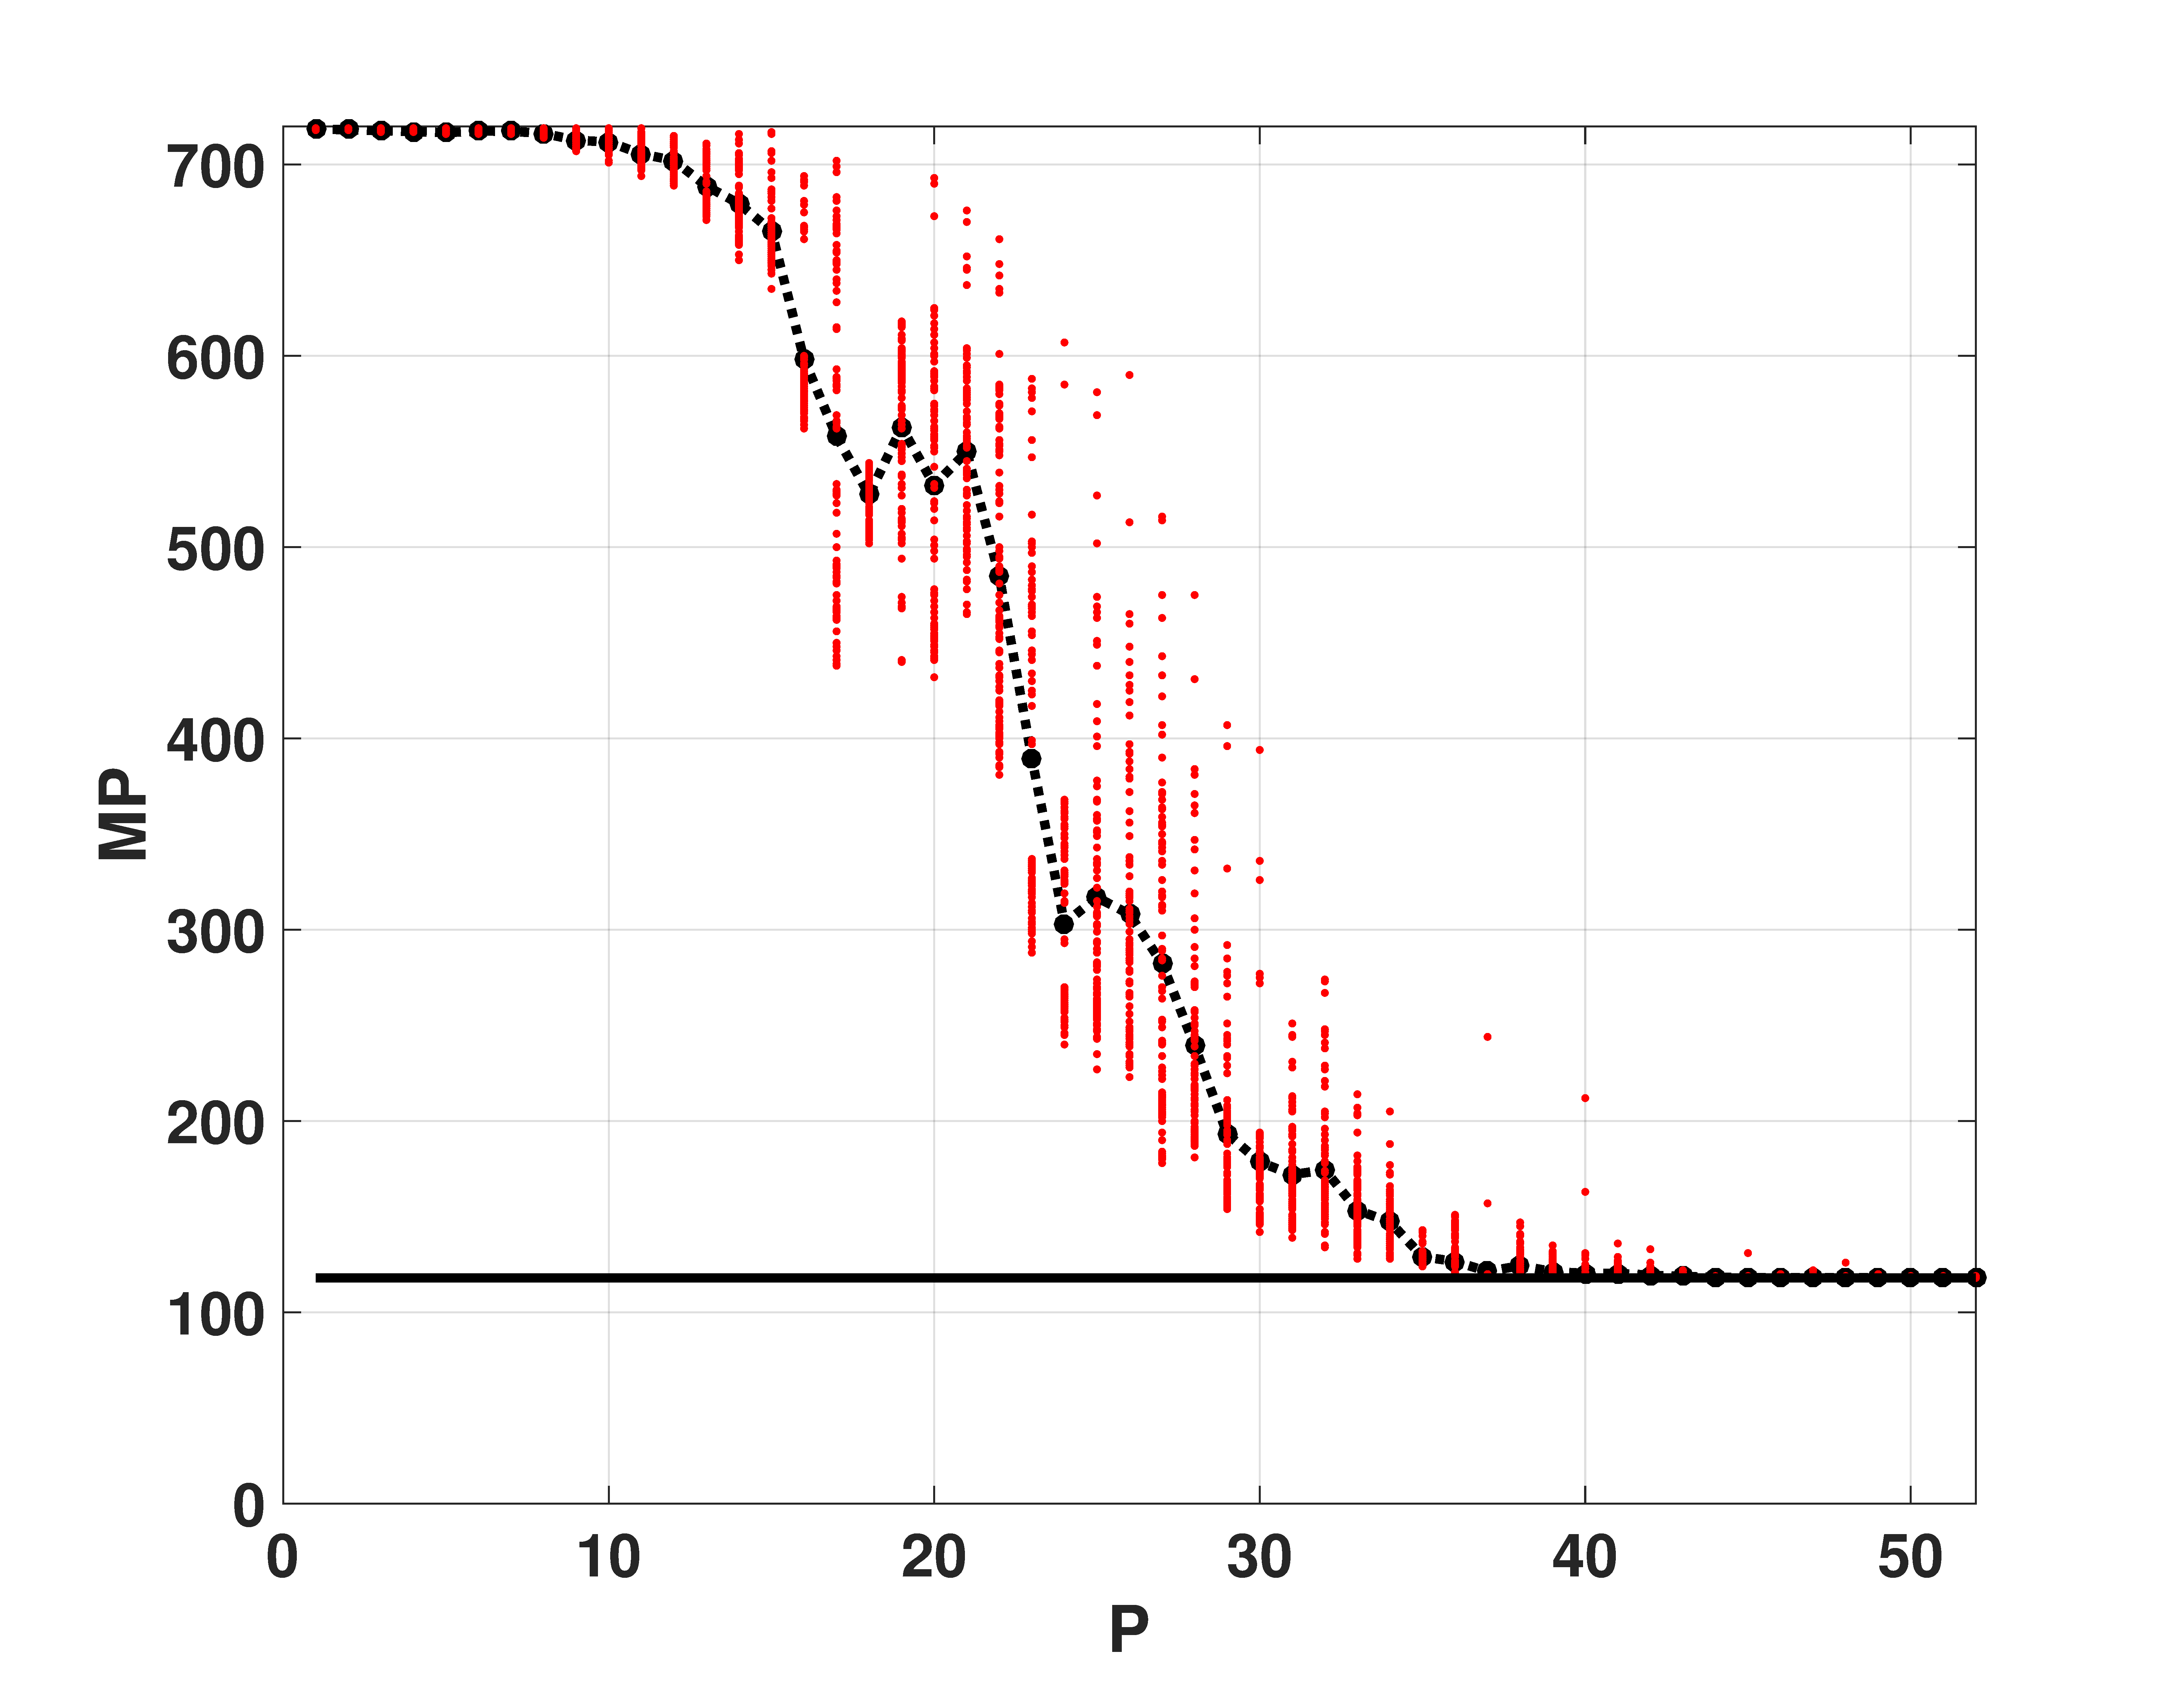
\includegraphics[width=.32\textwidth]{MP_SwitchOdd}
	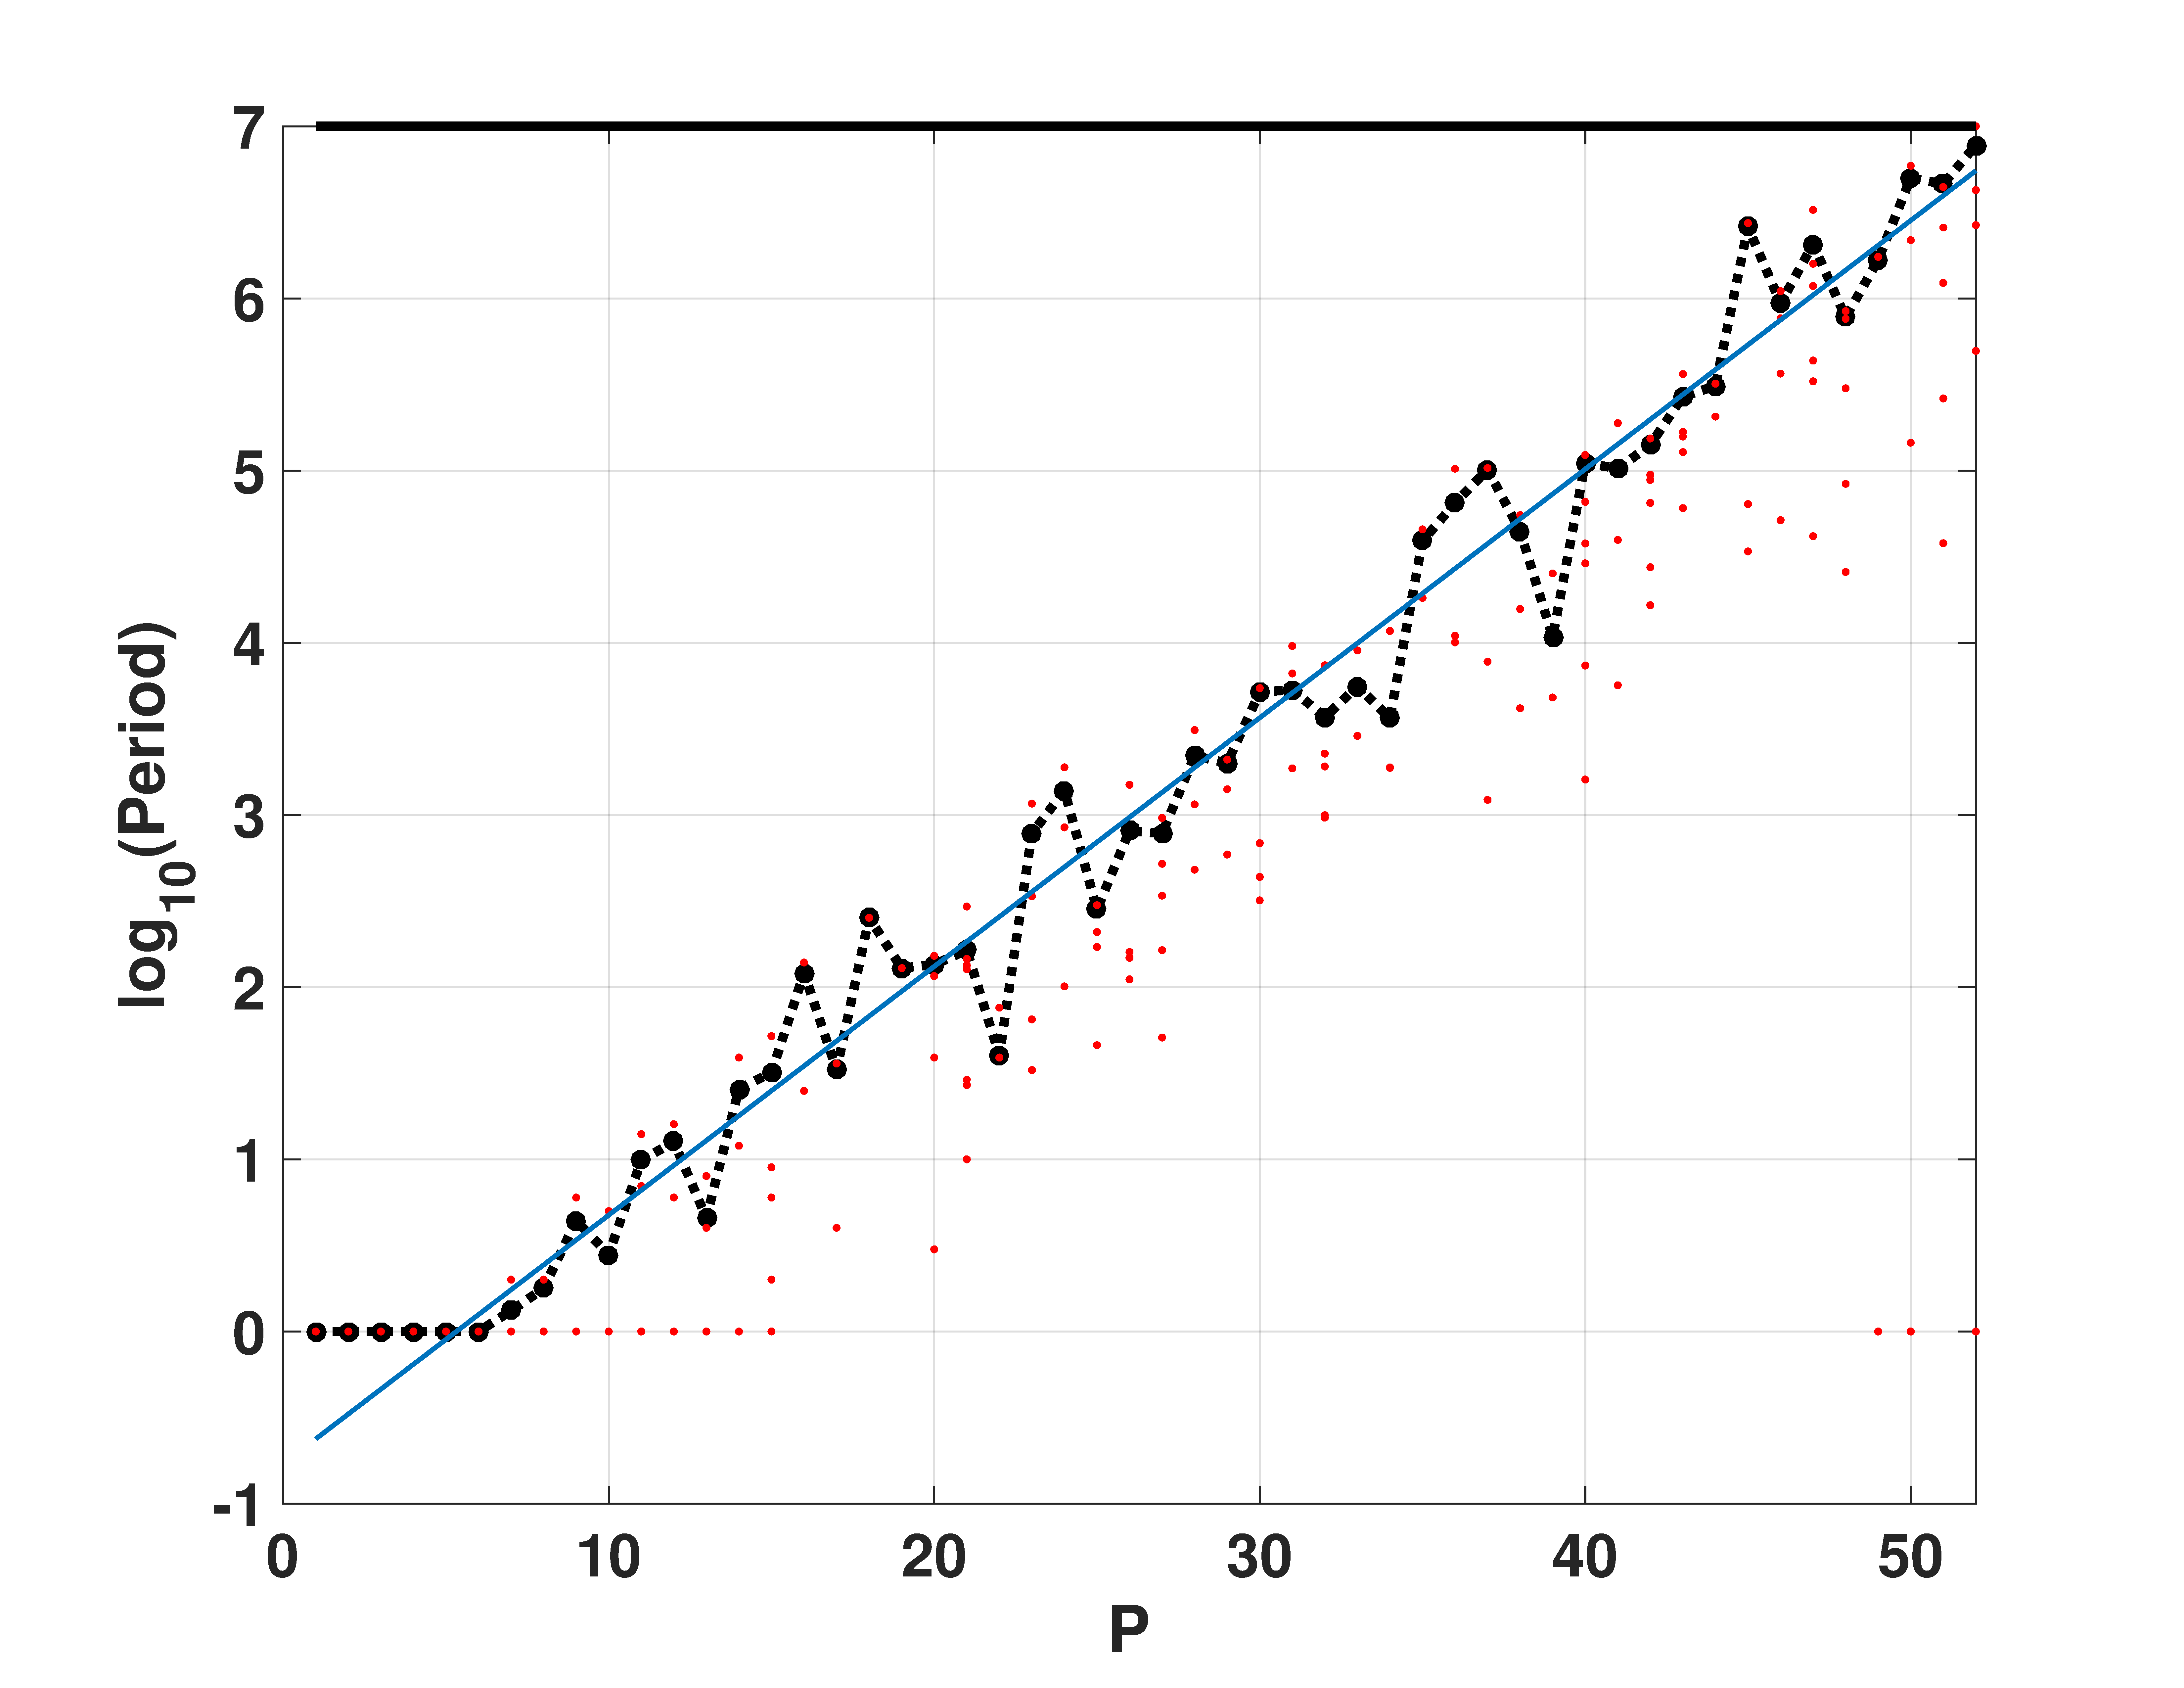
\includegraphics[width=.32\textwidth]{Period_SwitchOdd}
	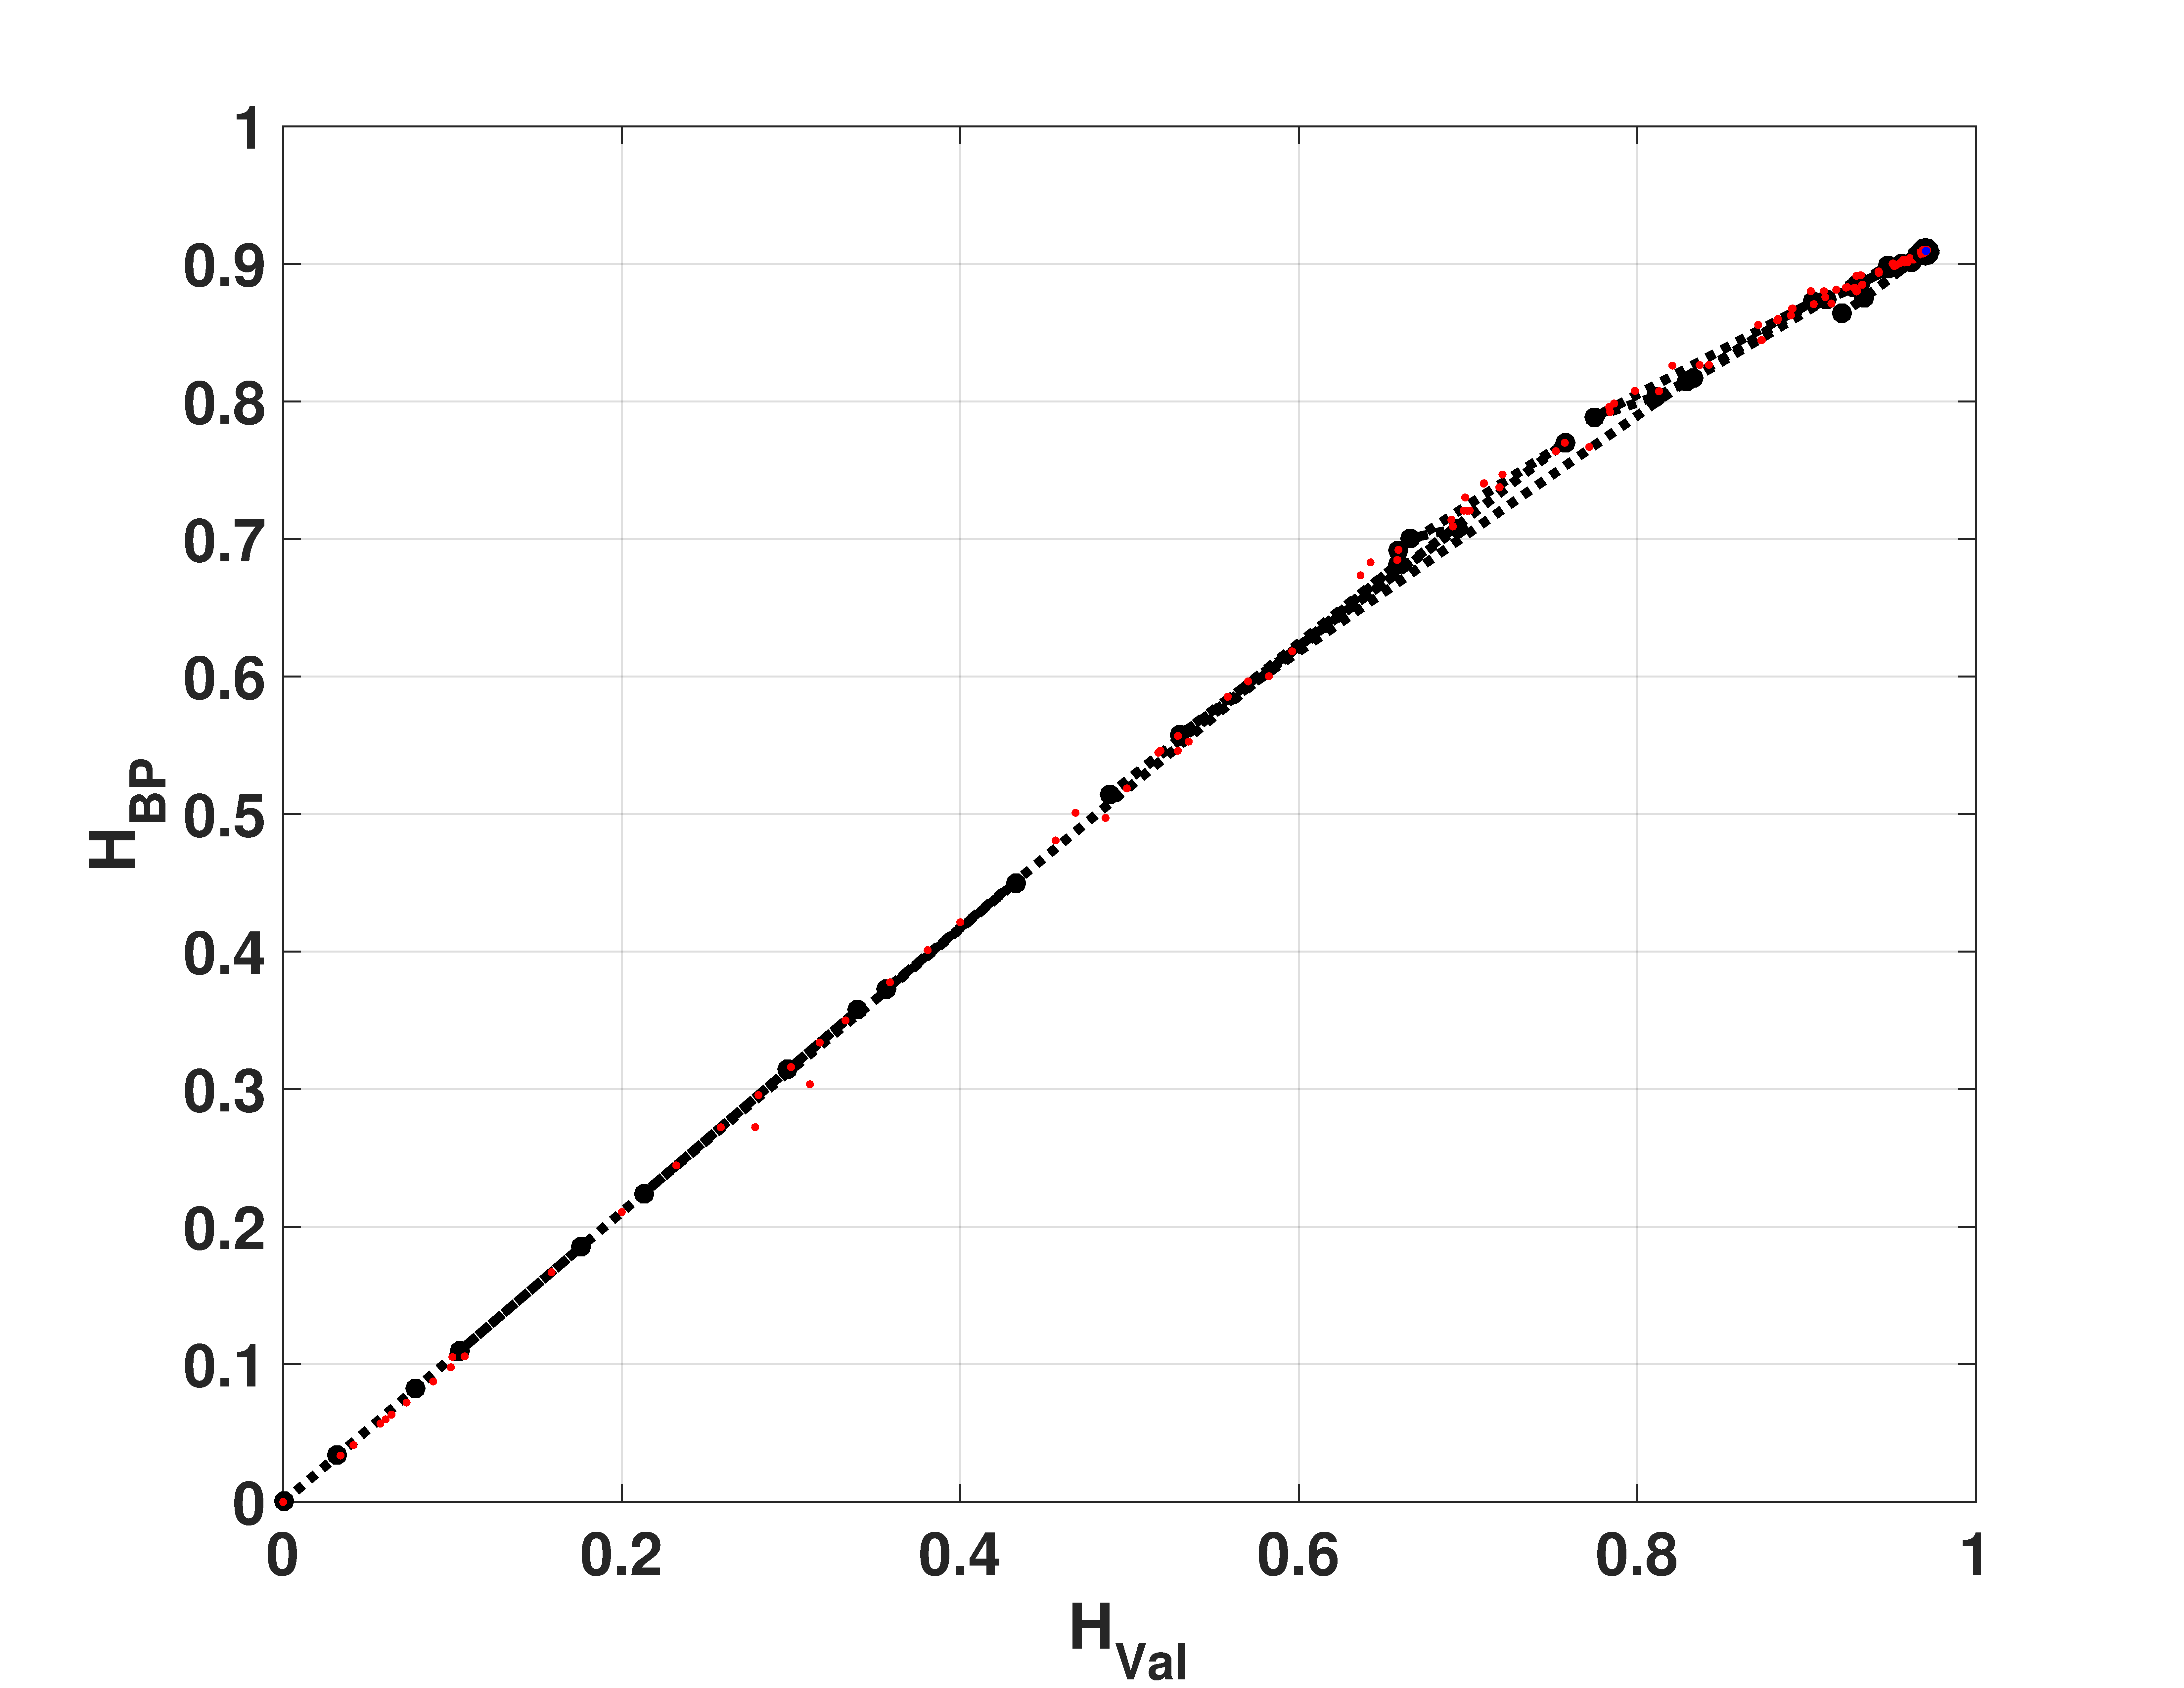
\includegraphics[width=.32\textwidth]{HbpHval_SwitchOdd}
	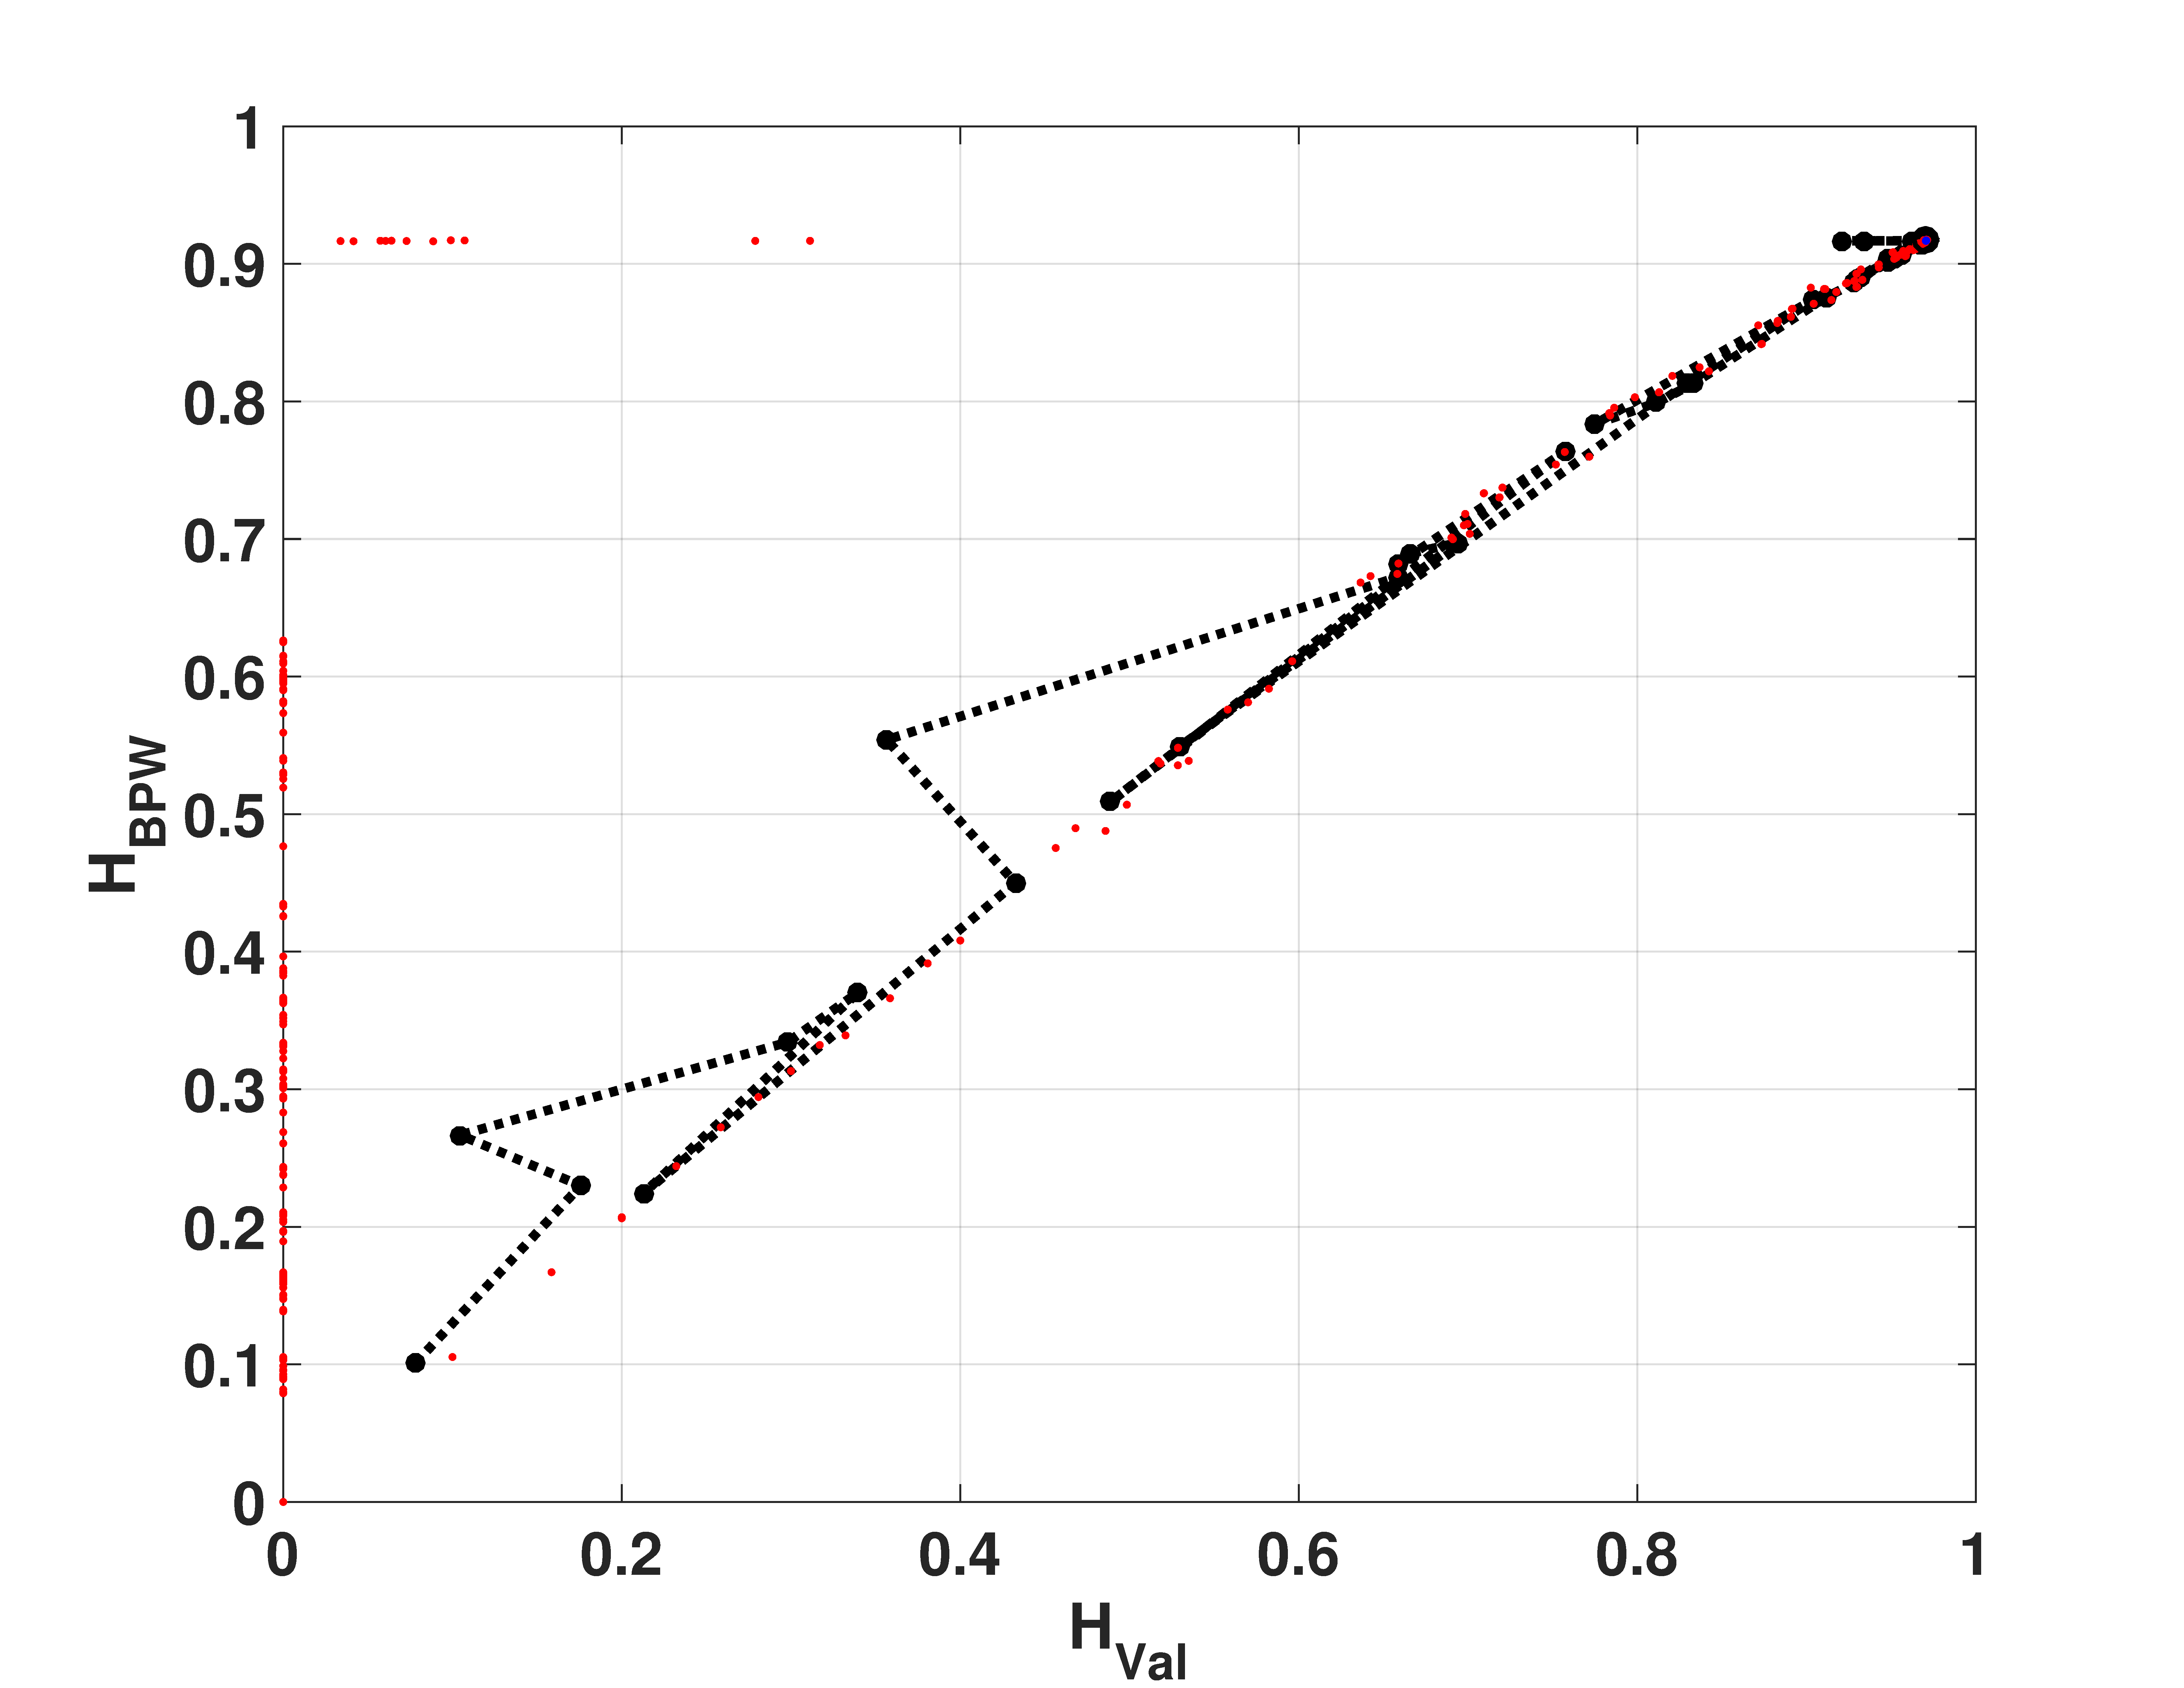
\includegraphics[width=.32\textwidth]{HbpwHval_SwitchOdd}
	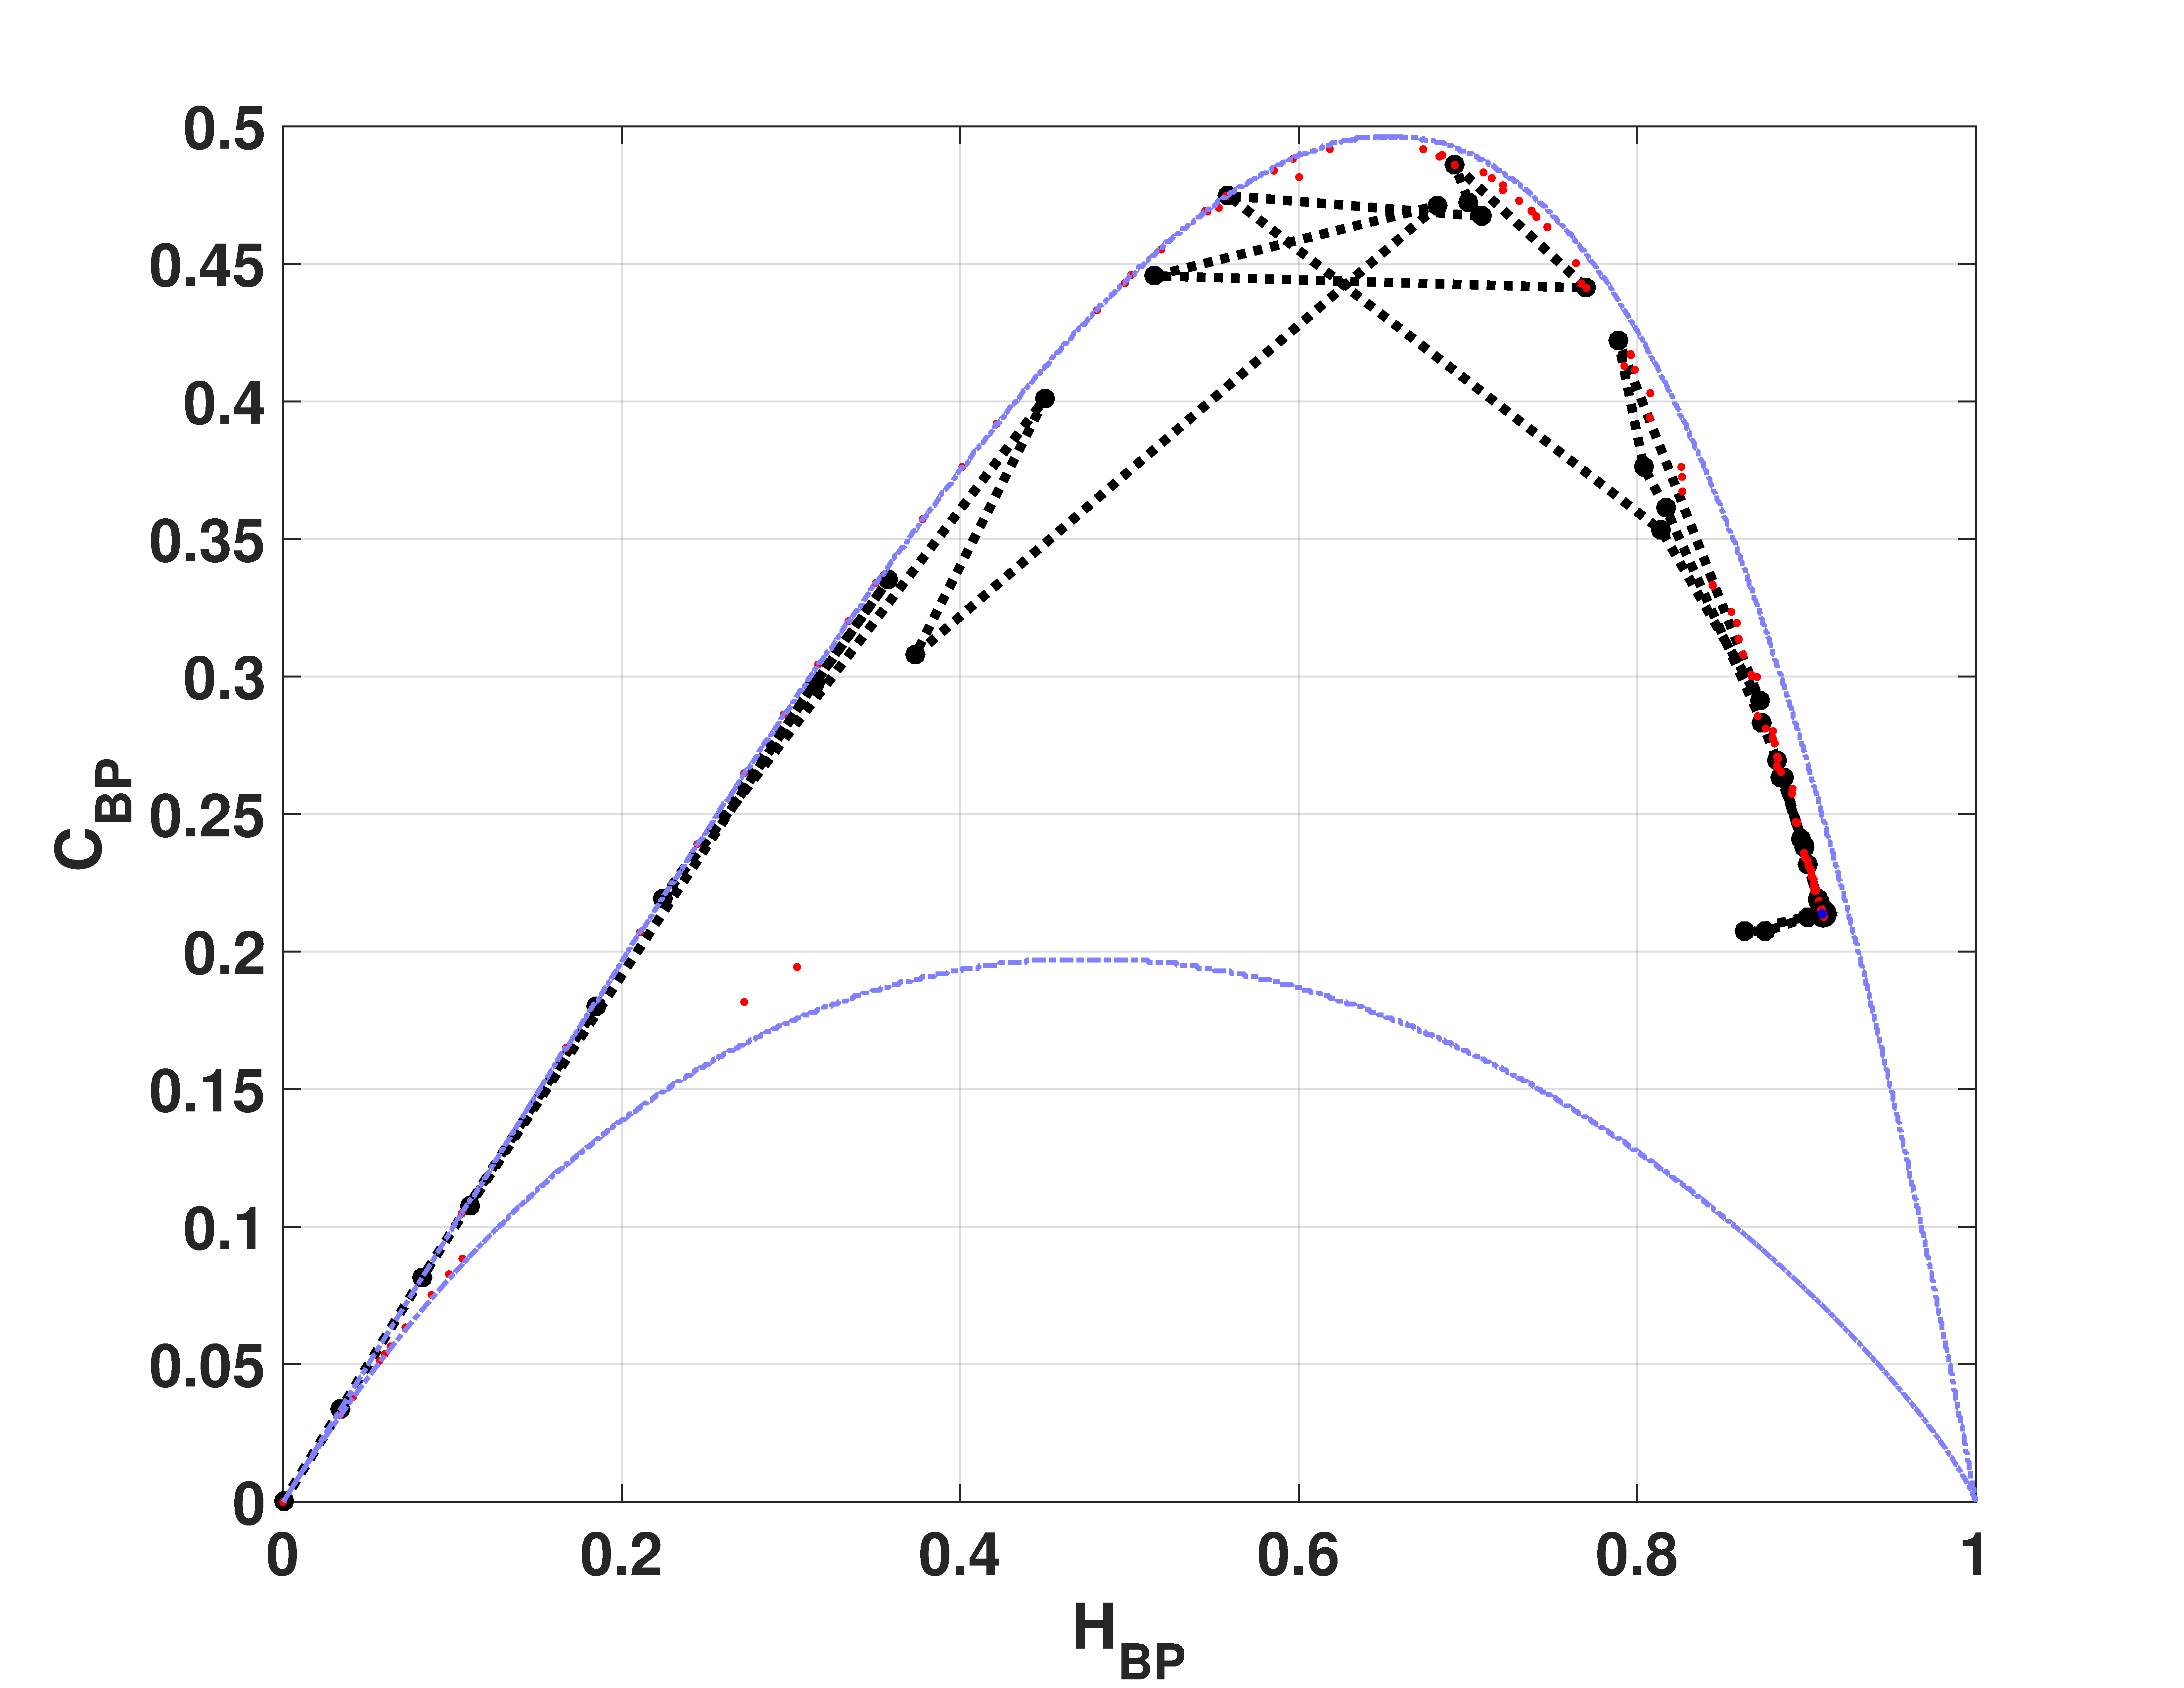
\includegraphics[width=.32\textwidth]{CbpHbp_SwitchOdd}
	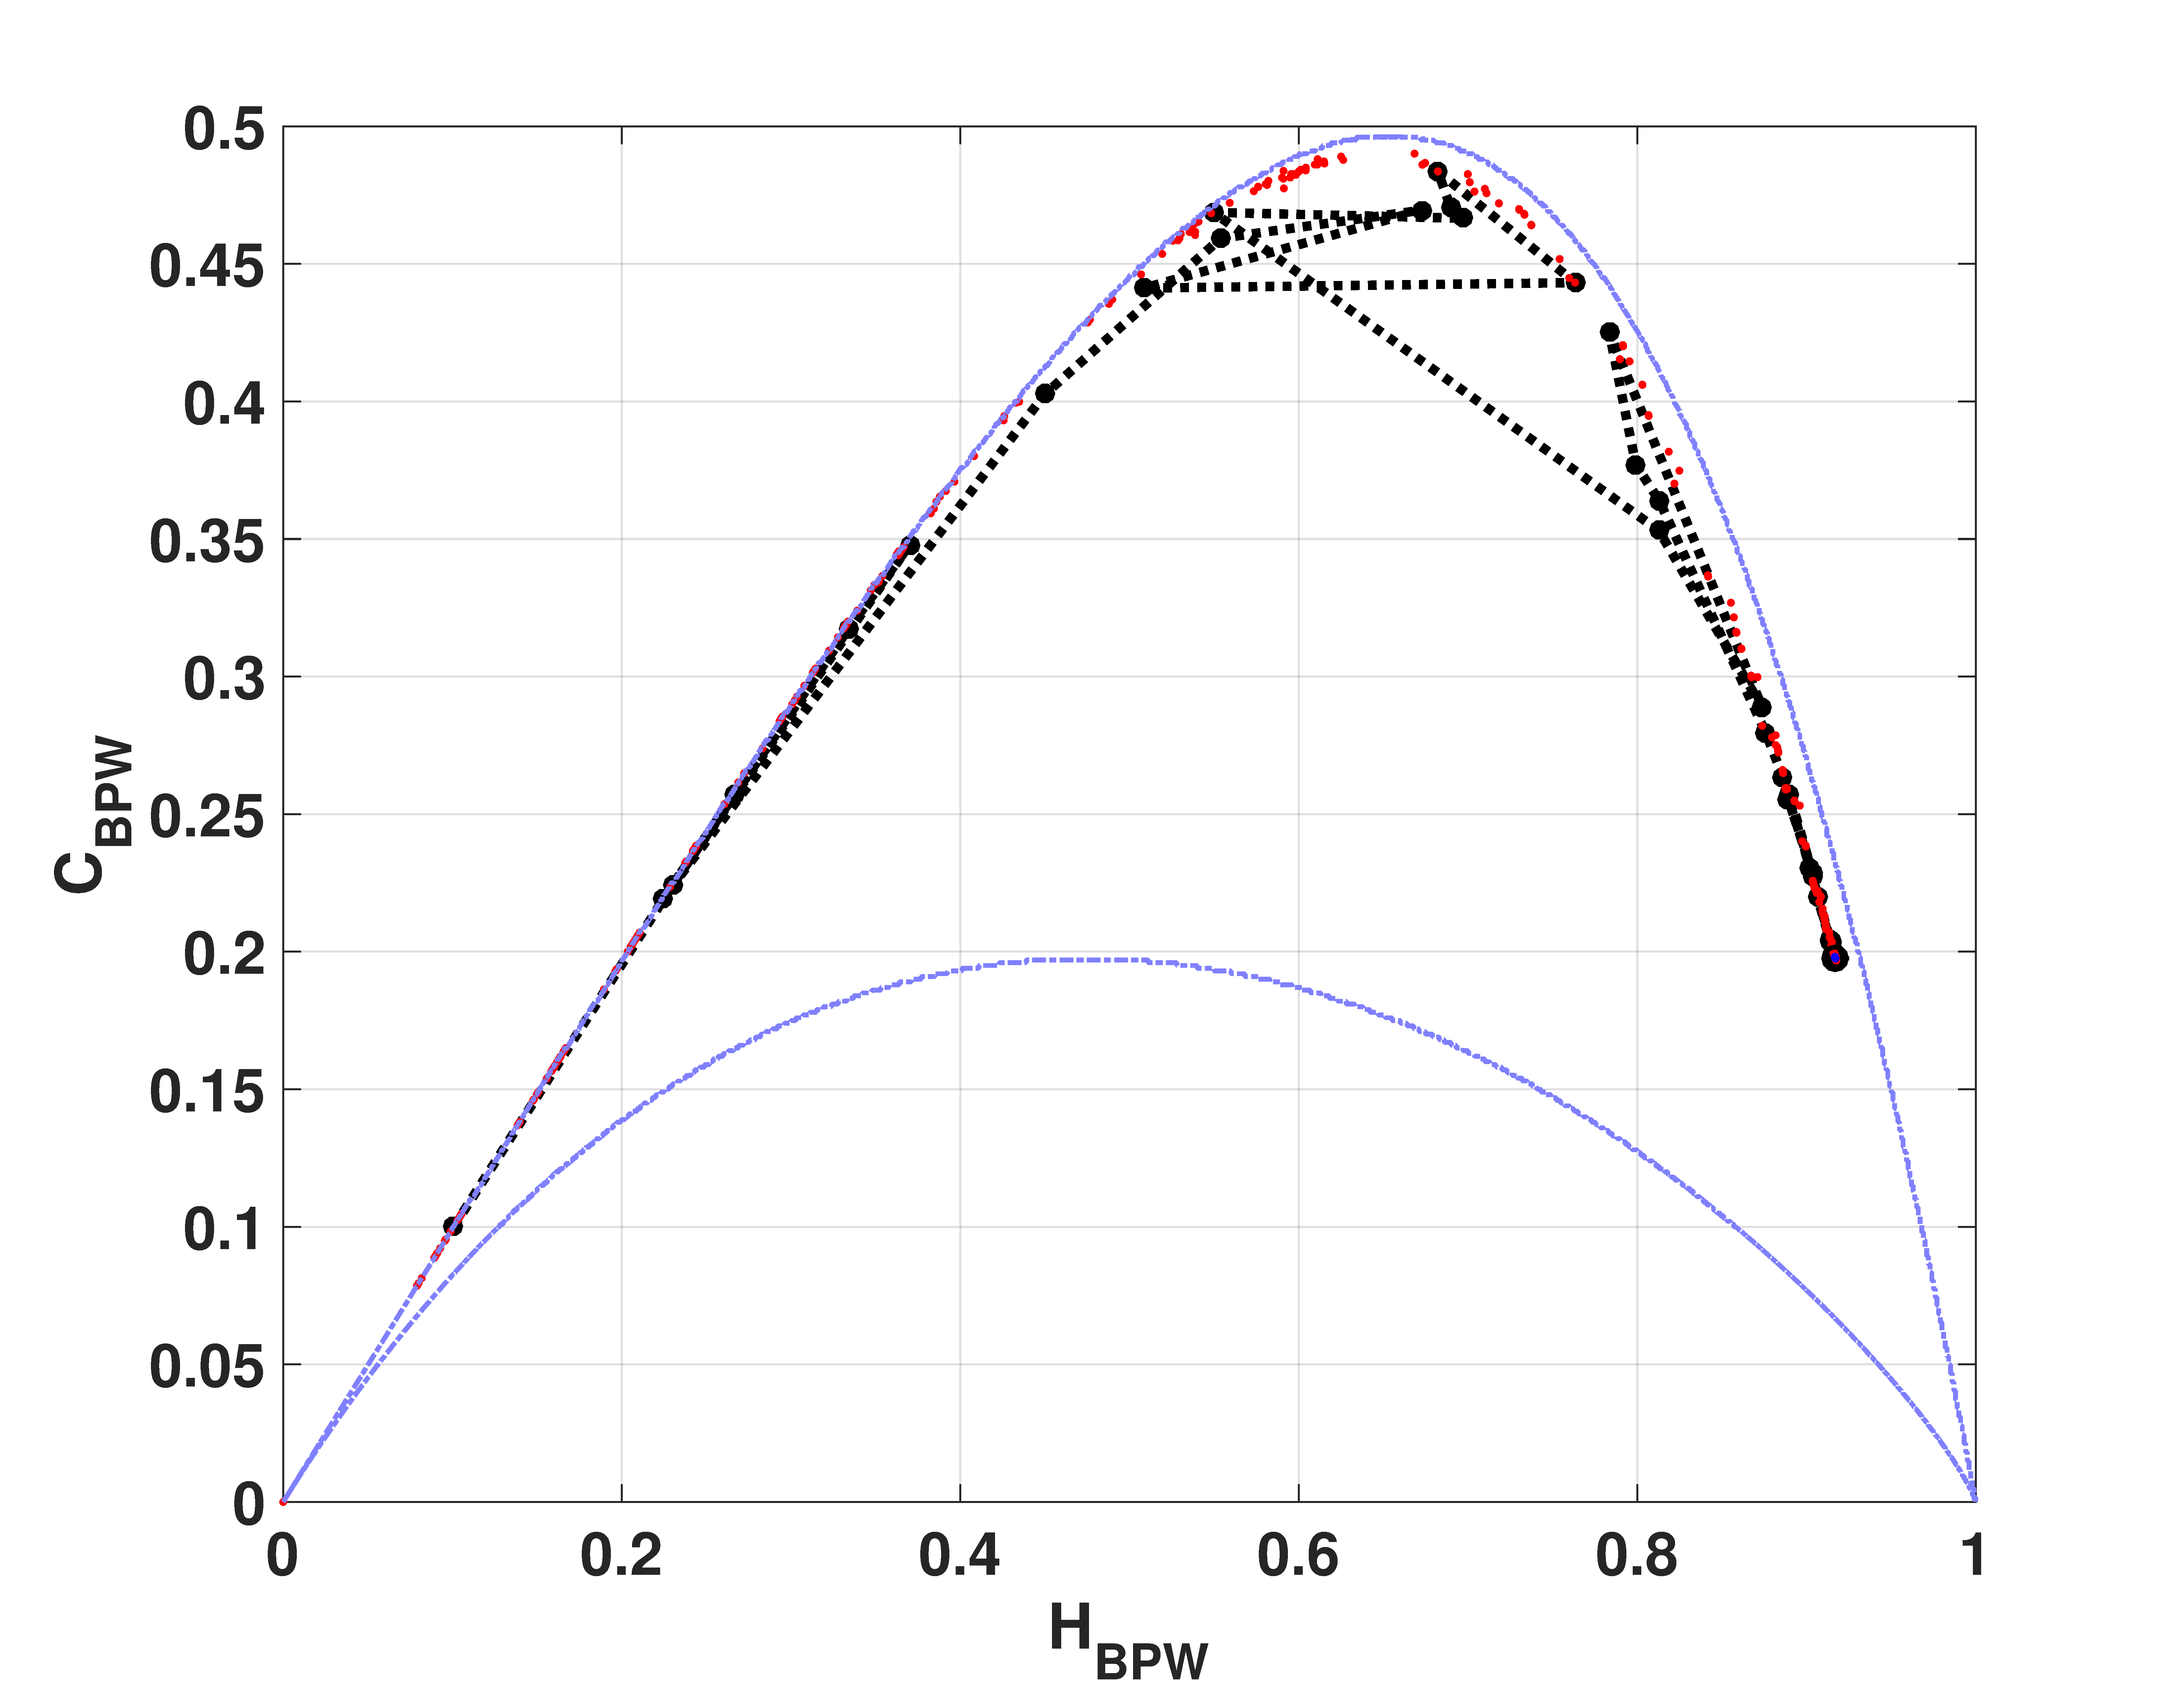
\includegraphics[width=.32\textwidth]{CbpwHbpw_SwitchOdd}
	\caption{Statistical properties of EVEN, obtained by skipping the values in the odd position of the time series of  SWITCH,  using binary representation: (a) $H_{hist}$ vs $P$ (b) $H_{BP}$ vs $P$ (c) $C_{BP}$ vs $P$ (d) Number of missing ordering patterns $MP$ vs $P$. In Figures (a) to (d) dashed line correspond to floating point numbers. (e) representation in the $H_{hist},H_{BP}$ plane in the the binary numerical system.  The star represents the state for floating points numbers. (f) representation in the $H_{BP},C_{BP}$ plane.  The star represents the state for floating points numbers.  } \label{fig:seqimparbin}
\end{figure}